%\VignetteIndexEntry{Statistical Working Paper on Imputation Methodology for the FAOSTAT Production Domain}
%\VignetteEngine{knitr::knitr}
\documentclass[nojss]{jss}\usepackage[]{graphicx}\usepackage[]{color}
%% maxwidth is the original width if it is less than linewidth
%% otherwise use linewidth (to make sure the graphics do not exceed the margin)
\makeatletter
\def\maxwidth{ %
  \ifdim\Gin@nat@width>\linewidth
    \linewidth
  \else
    \Gin@nat@width
  \fi
}
\makeatother

\definecolor{fgcolor}{rgb}{0.345, 0.345, 0.345}
\newcommand{\hlnum}[1]{\textcolor[rgb]{0.686,0.059,0.569}{#1}}%
\newcommand{\hlstr}[1]{\textcolor[rgb]{0.192,0.494,0.8}{#1}}%
\newcommand{\hlcom}[1]{\textcolor[rgb]{0.678,0.584,0.686}{\textit{#1}}}%
\newcommand{\hlopt}[1]{\textcolor[rgb]{0,0,0}{#1}}%
\newcommand{\hlstd}[1]{\textcolor[rgb]{0.345,0.345,0.345}{#1}}%
\newcommand{\hlkwa}[1]{\textcolor[rgb]{0.161,0.373,0.58}{\textbf{#1}}}%
\newcommand{\hlkwb}[1]{\textcolor[rgb]{0.69,0.353,0.396}{#1}}%
\newcommand{\hlkwc}[1]{\textcolor[rgb]{0.333,0.667,0.333}{#1}}%
\newcommand{\hlkwd}[1]{\textcolor[rgb]{0.737,0.353,0.396}{\textbf{#1}}}%

\usepackage{framed}
\makeatletter
\newenvironment{kframe}{%
 \def\at@end@of@kframe{}%
 \ifinner\ifhmode%
  \def\at@end@of@kframe{\end{minipage}}%
  \begin{minipage}{\columnwidth}%
 \fi\fi%
 \def\FrameCommand##1{\hskip\@totalleftmargin \hskip-\fboxsep
 \colorbox{shadecolor}{##1}\hskip-\fboxsep
     % There is no \\@totalrightmargin, so:
     \hskip-\linewidth \hskip-\@totalleftmargin \hskip\columnwidth}%
 \MakeFramed {\advance\hsize-\width
   \@totalleftmargin\z@ \linewidth\hsize
   \@setminipage}}%
 {\par\unskip\endMakeFramed%
 \at@end@of@kframe}
\makeatother

\definecolor{shadecolor}{rgb}{.97, .97, .97}
\definecolor{messagecolor}{rgb}{0, 0, 0}
\definecolor{warningcolor}{rgb}{1, 0, 1}
\definecolor{errorcolor}{rgb}{1, 0, 0}
\newenvironment{knitrout}{}{} % an empty environment to be redefined in TeX

\usepackage{alltt}
\usepackage{url}
\usepackage[sc]{mathpazo}
\usepackage{geometry}
\geometry{verbose,tmargin=2.5cm,bmargin=2.5cm,lmargin=2.5cm,rmargin=2.5cm}
\setcounter{secnumdepth}{2}
\setcounter{tocdepth}{2}
\usepackage{breakurl}
\usepackage{hyperref}
\usepackage[ruled, vlined]{algorithm2e}
\usepackage{mathtools}
\usepackage{draftwatermark}
\usepackage{float}
\usepackage{placeins}
\usepackage{mathrsfs}
\usepackage{multirow}
%% \usepackage{mathbbm}
\DeclareMathOperator{\sgn}{sgn}
\DeclareMathOperator*{\argmax}{\arg\!\max}







\title{\bf Statistical Working Paper on Imputation Methodology for the
  FAOSTAT Production Domain}

\author{Michael. C. J. Kao\\ Food and Agriculture Organization \\ of
  the United Nations}

\Plainauthor{Michael. C. J. Kao} 

\Plaintitle{Statistical Working Paper on Imputation Methodology for
  the FAOSTAT Production Domain}

\Shorttitle{Imputation Methodology}

\Abstract{ 


  This paper proposes a new imputation method for the FAOSTAT
  production domain based on linear mixed model and ensemble learning.
  
  The proposal provides resolve to many of the shortcomings of the
  current approach, and offers a flexible and robust framework to
  incorporate further information to improve performance.
  
  We begin with an exploration of three selected variables in the
  production domain and an attempt to pin point their potential
  drivers. These provide supports and explainations to the newly
  proposed methodology.
  
  A detailed account of the methodologies is provided. The linear
  mixed model demonstrates ability to capture cross-country and
  cross-commodity information which are present in the yield
  series. On the other hand, the ensemble learning display flexible
  yet robust characteristics for the imputation of the production
  where traditional method of applying a single model will fail.
    
}

\Keywords{Imputation, Linear Mixed Model, Agricultural Production, Ensemble Learning}
\Plainkeywords{Imputation, Linear Mixed Model, Agricultural Production, Ensemble Learning}

\Address{
  Michael. C. J. Kao\\
  Economics and Social Statistics Division (ESS)\\
  Economic and Social Development Department (ES)\\
  Food and Agriculture Organization of the United Nations (FAO)\\
  Viale delle Terme di Caracalla 00153 Rome, Italy\\
  E-mail: \email{michael.kao@fao.org}\\
  URL: \url{https://github.com/mkao006/sws_imputation}
}
\IfFileExists{upquote.sty}{\usepackage{upquote}}{}
\begin{document}

\section*{Disclaimer}
This Working Paper should not be reported as representing the views of
the FAO. The views expressed in this Working Paper are those of the
author and do not necessarily represent those of the FAO or FAO
policy. Working Papers describe research in progress by the author and
are published to elicit comments and to further discussion.\\

It is in the view of the author that imputation should be implemented
as a last resort, rather as a replacement for data
collection. Imputation itself does not create information it merely
create observations based on assumption. \\

This paper is dynamically generated on \today{} and is subject to
changes and updates.

\section{Introduction}
Missing values are commonplace in the agricultural production domain,
stemming from non-response in surveys or a lack of capacity by the
reporting entity to provide measurement. Yet a consistent and
non-sparse production domain is of critical importance to Food Balance
Sheets (FBS), thus accurate and reliable imputation is essential and a
necessary requisite for continuing work. This paper addresses several
shortcomings of the current work and a new methodology is proposed in
order to resolve these issues and to increase the accuracy of
imputation.\\

The relationship between the variables in the production domain by
definition can be expressed as follow,

\begin{equation}
  \label{eq:identity}
  \text{P}_t := \text{A}_t \times \text{Y}_t \quad\quad P_t \ge 0,\, A_t
  \ge 0,\, Y_t > 0
\end{equation}


Where $P$, $A$ and $Y$ represent production, area harvested and yield
of crops, respectively, indexed by time $t$. In the case of livestock,
$A$ represents number of slaughtered animal while $Y$ represents the
carcass weight per animal. The yield is, however, unobserved and can
only be calculated when both production and area are available. For
certain commodities, harvested area may not exist or sometimes it may
be represented under a different context.\\

It is important to recognize that when area harvested and production
are both zero, yield is undefined. Yield is a derived statistic, and
when we can not observe it through calculation it does not imply it is
zero. In fact, it is a missing value by the very nature of the
definition being unobservable yet a value does exist.\\

The primary objective of imputation is to incorporate all
available and reliable information in order to provide best estimates of
food supply in FBS.\\

Presented in table \ref{tab:swsflag} is a description of the existing
flags in the current Statistical Working System (SWS). In this
exercise, estimated and previously imputed data which are marked as
either \textbf{F}, \textbf{E} and \textbf{T} are the target values to
be imputed.\\

\begin{table}[h!]
  \label{tab:swsflag}
  \caption{Description of the flags in the Statistical Working System}
  \begin{center}
    \begin{tabular}{|c||p{12cm}|}
      \hline
      Flags & Description\\
      \hline
      & Official data reported on FAO Questionnaires from countries\\
      / & Official data reported on FAO Questionnaires from countries\\
      * & Commodity International Organizations\\
      X & Commodity International Organizations\\
      P & Estimated data using trading partners database\\
      F & FAO estimate\\
      C & Calculated data\\
      B & Data obtained as balance\\
      T & Extrapolated/interpolated\\
      M & Not reported by country\\
      E & Expert sources from FAO (including other divisions)\\
      \hline
    \end{tabular}
  \end{center}  
\end{table}

\subsection{Scope of the project}
%% Need to check 
A total of 247 commodities requires imputation, 169 commodities from
the crop domain, 19 in primary livestock and 59 processed
livestock. There are in total of 245 countries including obsolete
classifications and territories which result in more than 180,000+
potential times series to impute.\\


\FloatBarrier
\section{Background and Review of the Current Methodology}

There have been two classes of methodology proposed in the past in
order to account for missing values in the production domain. The
first type utilizes historical information and implements methods such
as linear interpolation and trend regression; while the second class
aims to capture the variation of relevant commodity
and/or spatial characteristics through the application of
aggregated growth rates. The imputation is carried out independently
on both area and production, with the yield calculated implicitly as
an identity.\\

Nevertheless, both approaches only utilize one dimension of
information and improvements can be obtained if information usage
can be married. Furthermore, these methods lack the ability to
incorporate external information such as vegetation indices,
precipitation or temperature that may provide valuable information and
enhance the accuracy of imputation.\\

Simulation results of the prior attempts indicate that linear
interpolation over small period is a stable and accurate method but it
lacks the capability to utilize cross-sectional
information. Furthermore, it does not provide a solution for
extrapolation where connection points are not available. As a result,
the aggregation method was then implemented as it was found to provide
a high coverage rate for imputation with seemingly satisfactory
performance.\\

In short, the aggregation imputation method computes the
commodity/regional aggregated growth of both area and production, the
growth rate is then applied to the last observed value of the
respective series. The formula of the aggregated growth can be
expressed as:

\begin{equation}
  \label{eq:aggregateGrowth}
  r_{s, t} = \sum_{c \in \mathbb{S}} X_{c, t}/\sum_{c \in \mathbb{S}} X_{c, t-1}
\end{equation}

Where $\mathbb{S}$ denotes the relevant set of products and countries
within the relevant commodity group and regional classification after
omitting the item to be imputed. For example, to compute the
\textit{country cereal aggregated growth} with the aim to impute wheat
production, we sum up all the production of commodities listed in the
cereal group in the same country excluding wheat. On the other hand,
to impute by \textit{regional item aggregated growth}, wheat
production data within the regional profile except the country of
interest are aggregated.\\


Imputation can then be computed as:
\begin{equation}
  \hat{X}_{c, t} = X_{c, t-1} \times r_{s, t}
\end{equation}
  

There are, however, several shortcomings of this methodology. The
Achilles heel lies in the fact that area and production are imputed
independently, cases of diverging area harvested and production have
been observed that result in inconsistency between trends as well as
exploding yields. The source of this undesirable characteristic is
nested in the computation of the aggregated growth rate. Owing to
missing values, the basket computed may not be comparable over time
and consequently results in spurious growth or
contraction. Furthermore, the basket to compute the changes in
production and area may be considerably different.\\


\section{Exploratory Data Analysis}

We first take a visualization tour of the data to grasp an
understanding of the underlying pattern of the production domain and
the relationship between the variables. The series commence in 1992
and continues to 2011.

\subsection{Yield}

The next three graph depicts the yield of four selected commodity from
different commodity group, wheat, grape, okra and beef.\\


From the graphs, we can first observe that there is a general
increasing trend in the yield accross all countries and commodities
illustrated. Similar stories are observed in almost all commodities
that has been studied during the development of the methodology. This
is a result of continuous advancement in both technology and
agricultural practice driven by research \& development. Improved
irrigation provides crop with sufficient and uninterrupted water
source, while tailored compound feed provide the precise nutrient
requirements ensuring the livestocks consume the optimal diet for
growth. Regardless whether these practice are sustainable or
beneficial, there are strong evidence of increased productivity over
time.\\



Nevertheless, just like all available technology such as internet, the
distribution is far from perfect. The adoption of technology depends
on the access which may be hindered by the presence of patents, or
restriction imposed by service providers. Imperfect information and
limit financial resources are also major obstacles for embracing the
new developments, this is particularly true for countries where the
majority of the producers are smallholders or rural farming.\\

Furthermore, producers faces different constraints and cost. Countries
such as Brazil and Russia which has a large amount of arable land does
not bear the same cost for land acqusition in comparison to small
states such as the Netherlands. The cost translates to different
pressure to improve productivity and yield. Inovations required are
also different for countries, wheat breeding for the development of
drought and diease resistent variety were crucial to withold
Australia's dry climate.  \\


Despite the differences among the countries branching from various
combination of technological advancement and economic condition, these
factors all contribute towards a positive improvement in productitive
which can be estimated as an aggregated mixture effect.\\

Forces of nature also play a vital role in the determination of crop
productivity. However, unlike technological advancement, precipitation
and temperature are associated more closely to year-to-year variation.\\

\begin{knitrout}
\definecolor{shadecolor}{rgb}{0.969, 0.969, 0.969}\color{fgcolor}\begin{figure}[!ht]


{\centering 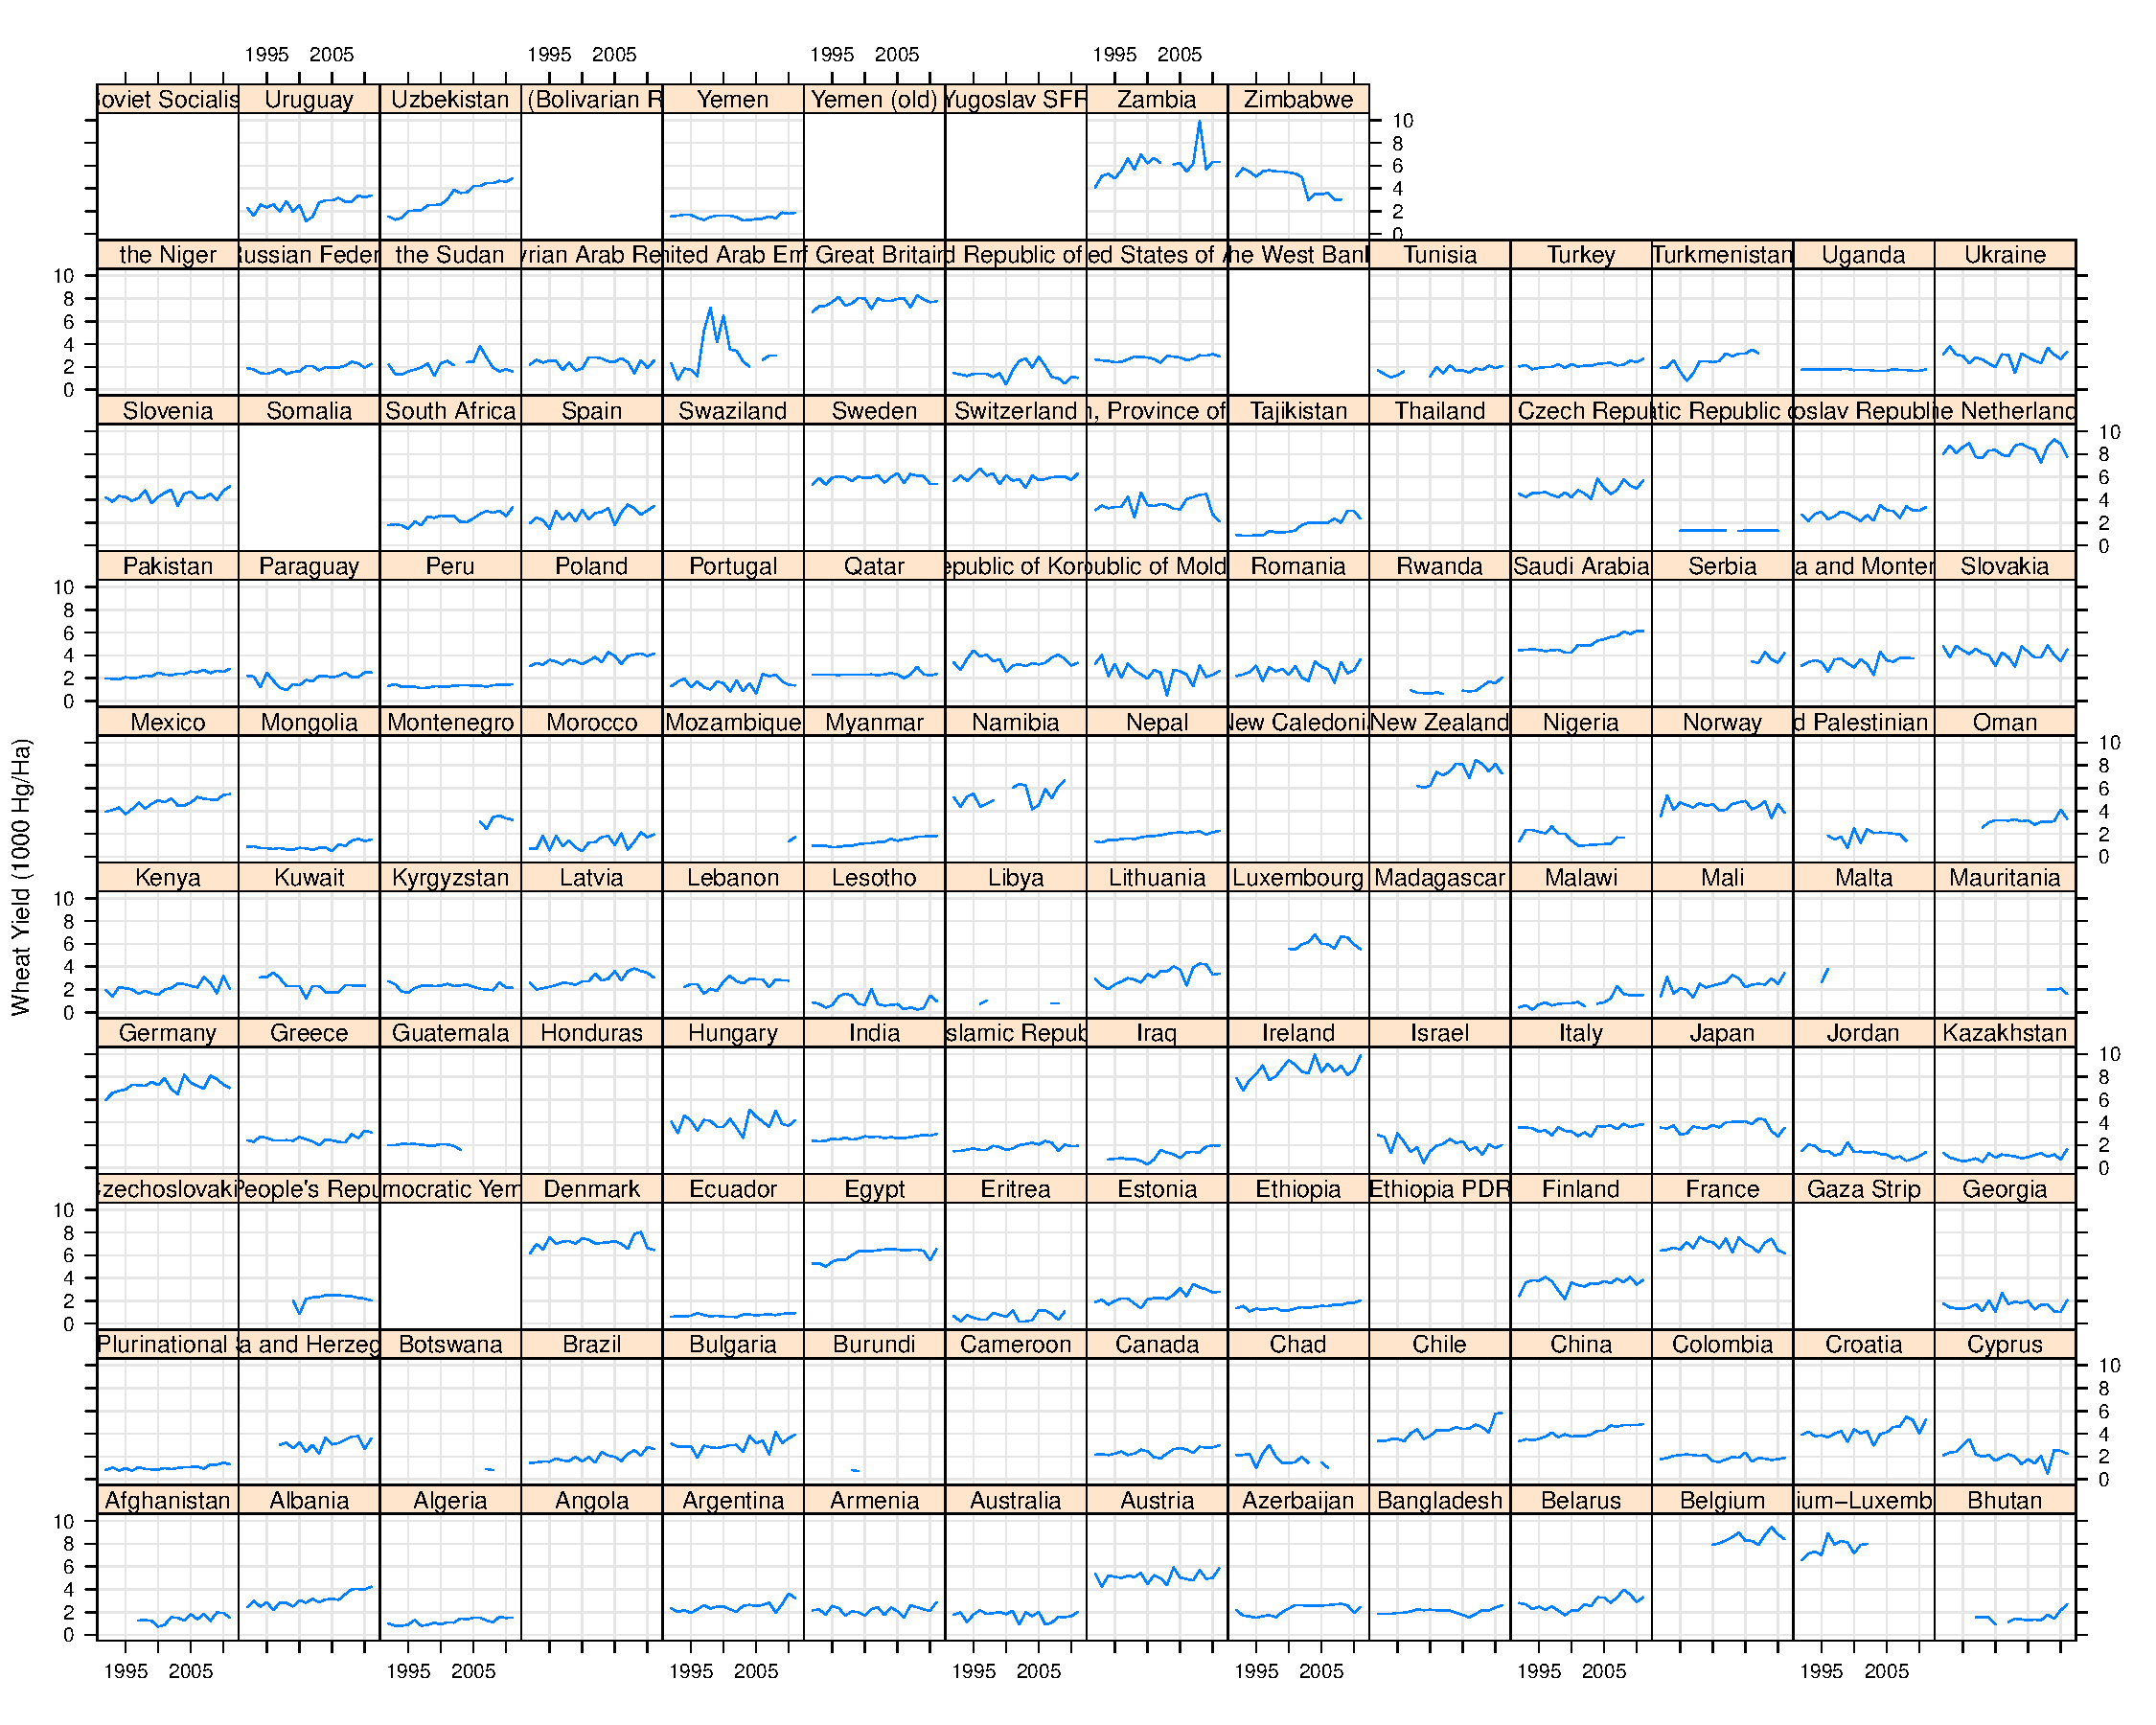
\includegraphics[width=\maxwidth]{figure/wheat-yield-explore} 

}

\caption[This figure illustrates the yield of wheat accross all countries, it provide strong support to the facts stated]{This figure illustrates the yield of wheat accross all countries, it provide strong support to the facts stated. First of all, we can observe the concordant increasing trend accross all country where technological innovation such as improved seed, and synthetic nitrogen fertilizer contributed to the increase in productivity. Yet at the same time, we can also observe that the rate of growth differ between countries. The single yield spike in Zambia raises concern on data quality.\label{fig:wheat-yield-explore}}
\end{figure}


\end{knitrout}





\begin{knitrout}
\definecolor{shadecolor}{rgb}{0.969, 0.969, 0.969}\color{fgcolor}\begin{figure}[!ht]


{\centering 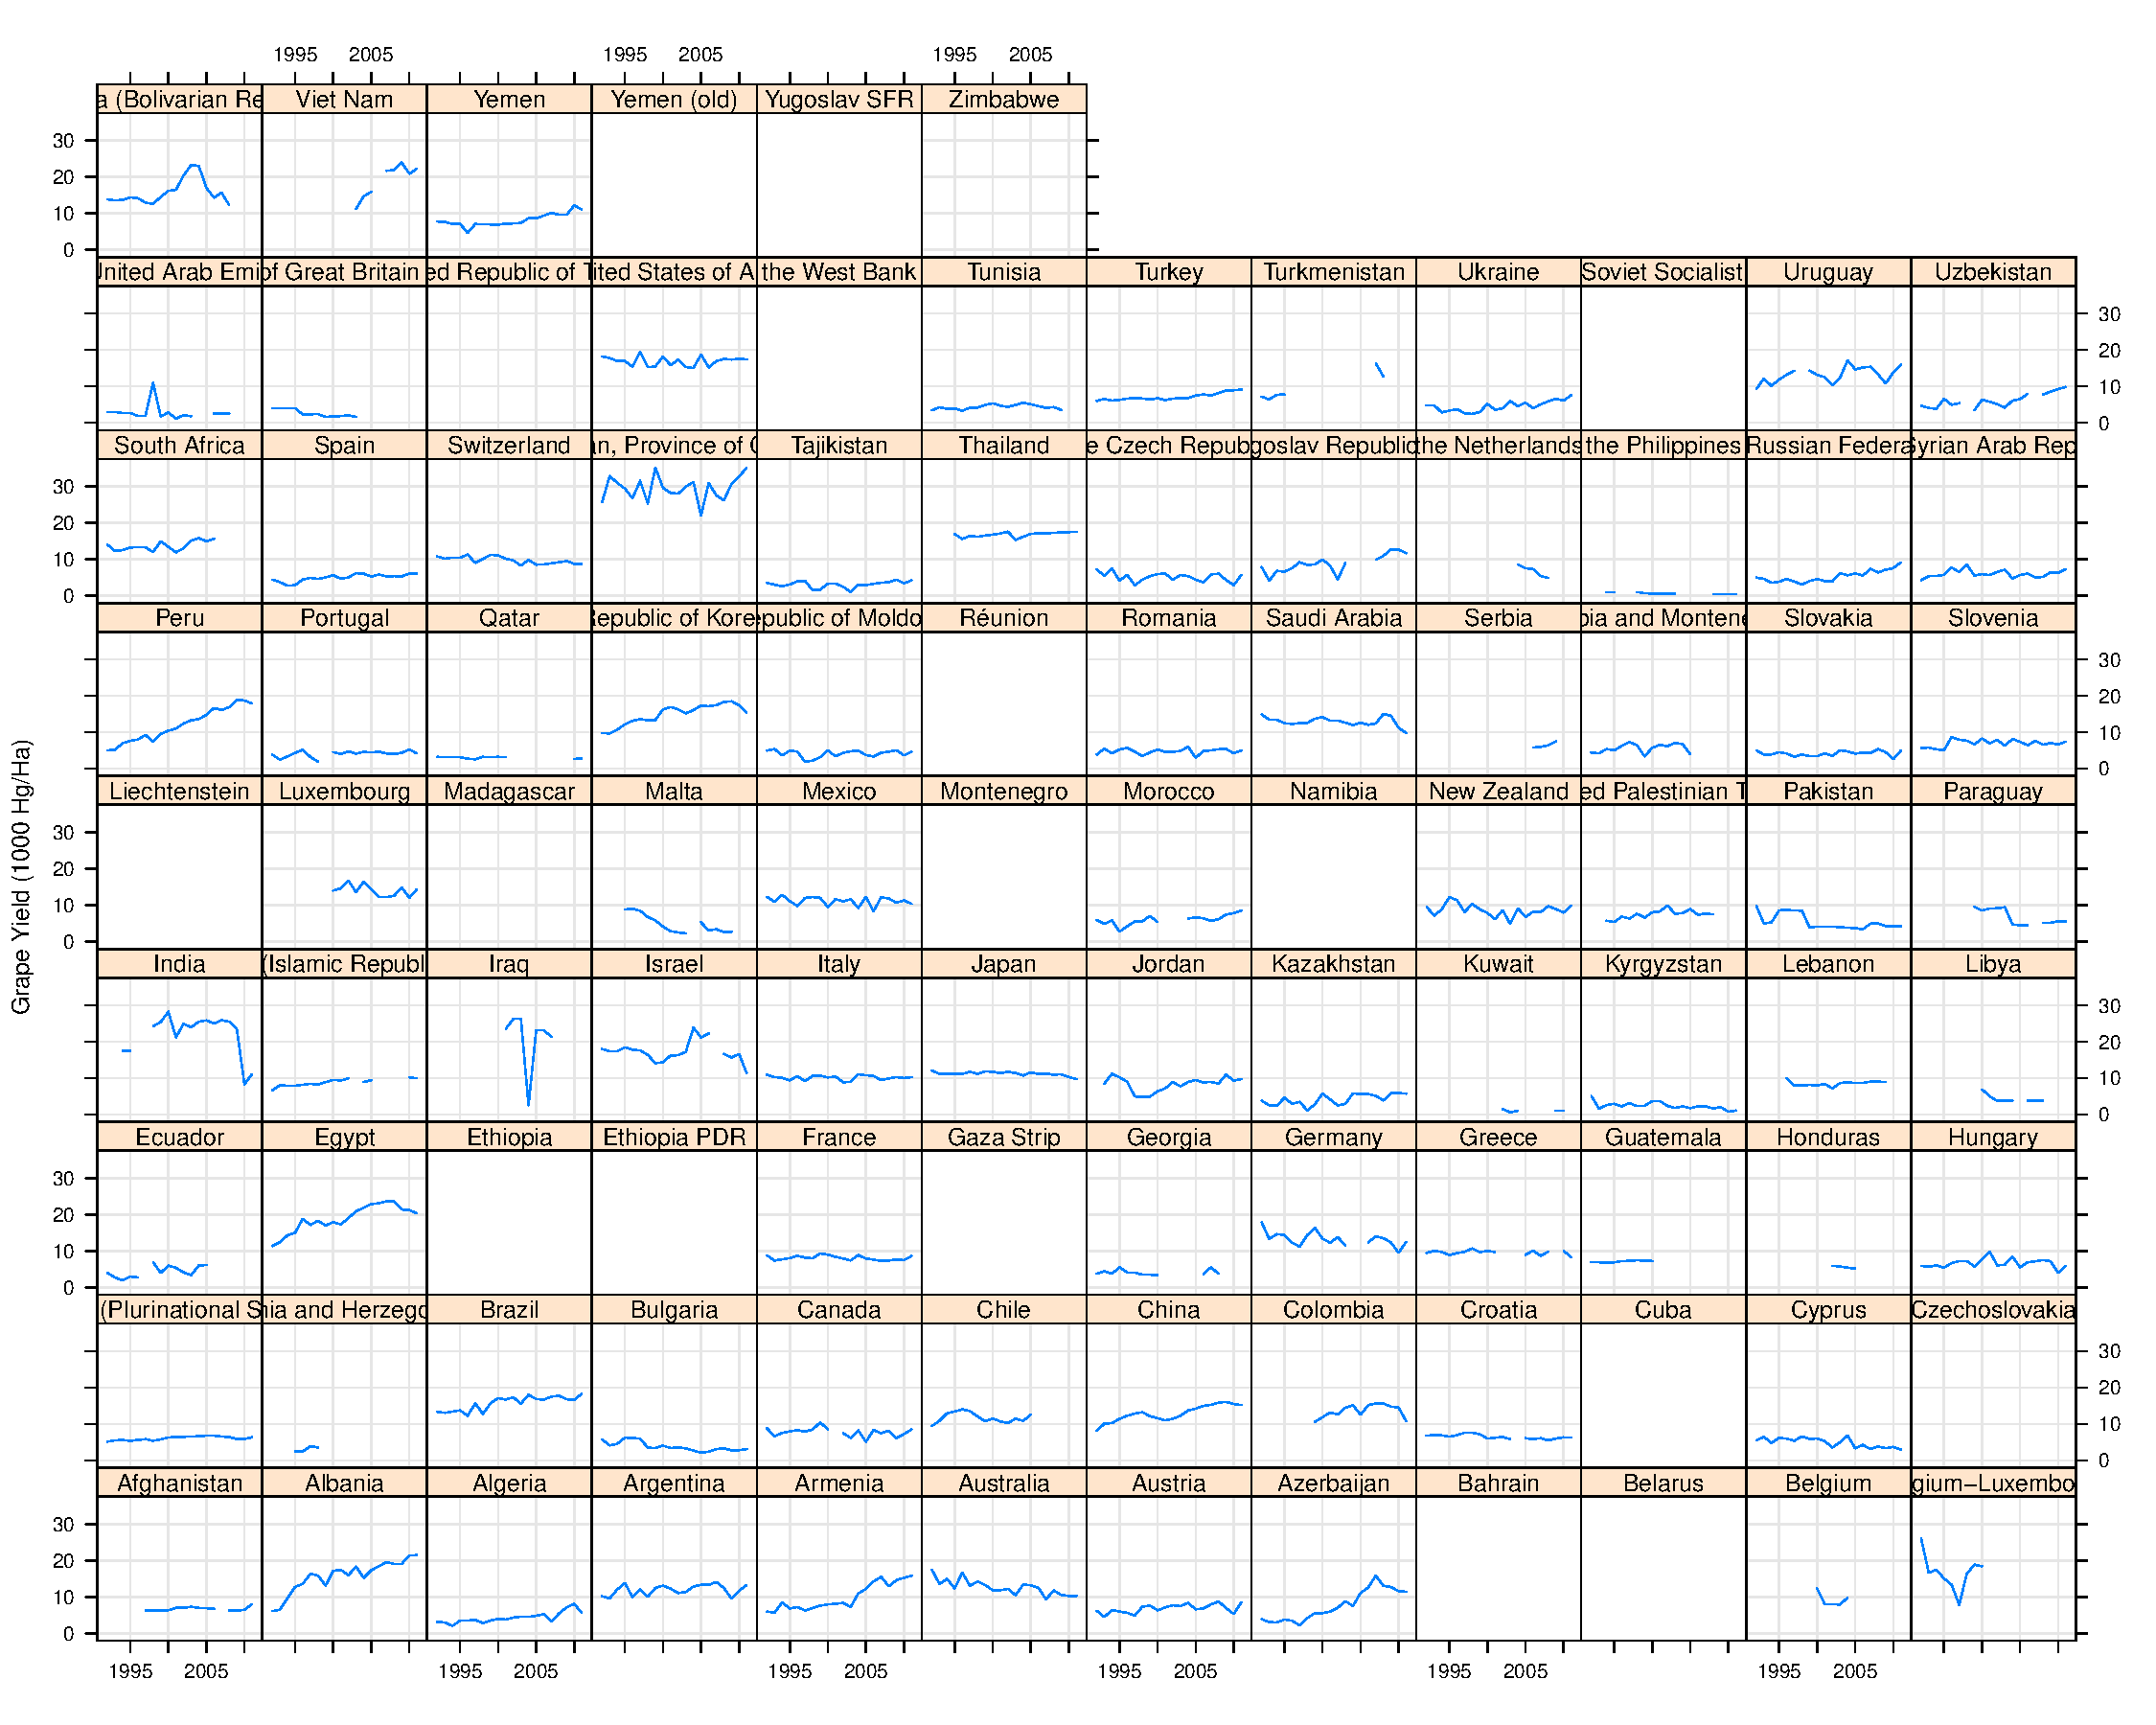
\includegraphics[width=\maxwidth]{figure/grape-yield-explore} 

}

\caption[Unlike the yield of wheat, the yield for grape has remain rather constant over time except a few selective country such as Peru and Azerbaijian]{Unlike the yield of wheat, the yield for grape has remain rather constant over time except a few selective country such as Peru and Azerbaijian. There are a few spikes observed, namely Iraq, the invasion of Iraq may have contributed to the negative shock. The considerable fall in the yield for India is of unknown cause, and potentially a data entry error.\label{fig:grape-yield-explore}}
\end{figure}


\end{knitrout}

\begin{knitrout}
\definecolor{shadecolor}{rgb}{0.969, 0.969, 0.969}\color{fgcolor}\begin{figure}[!ht]


{\centering 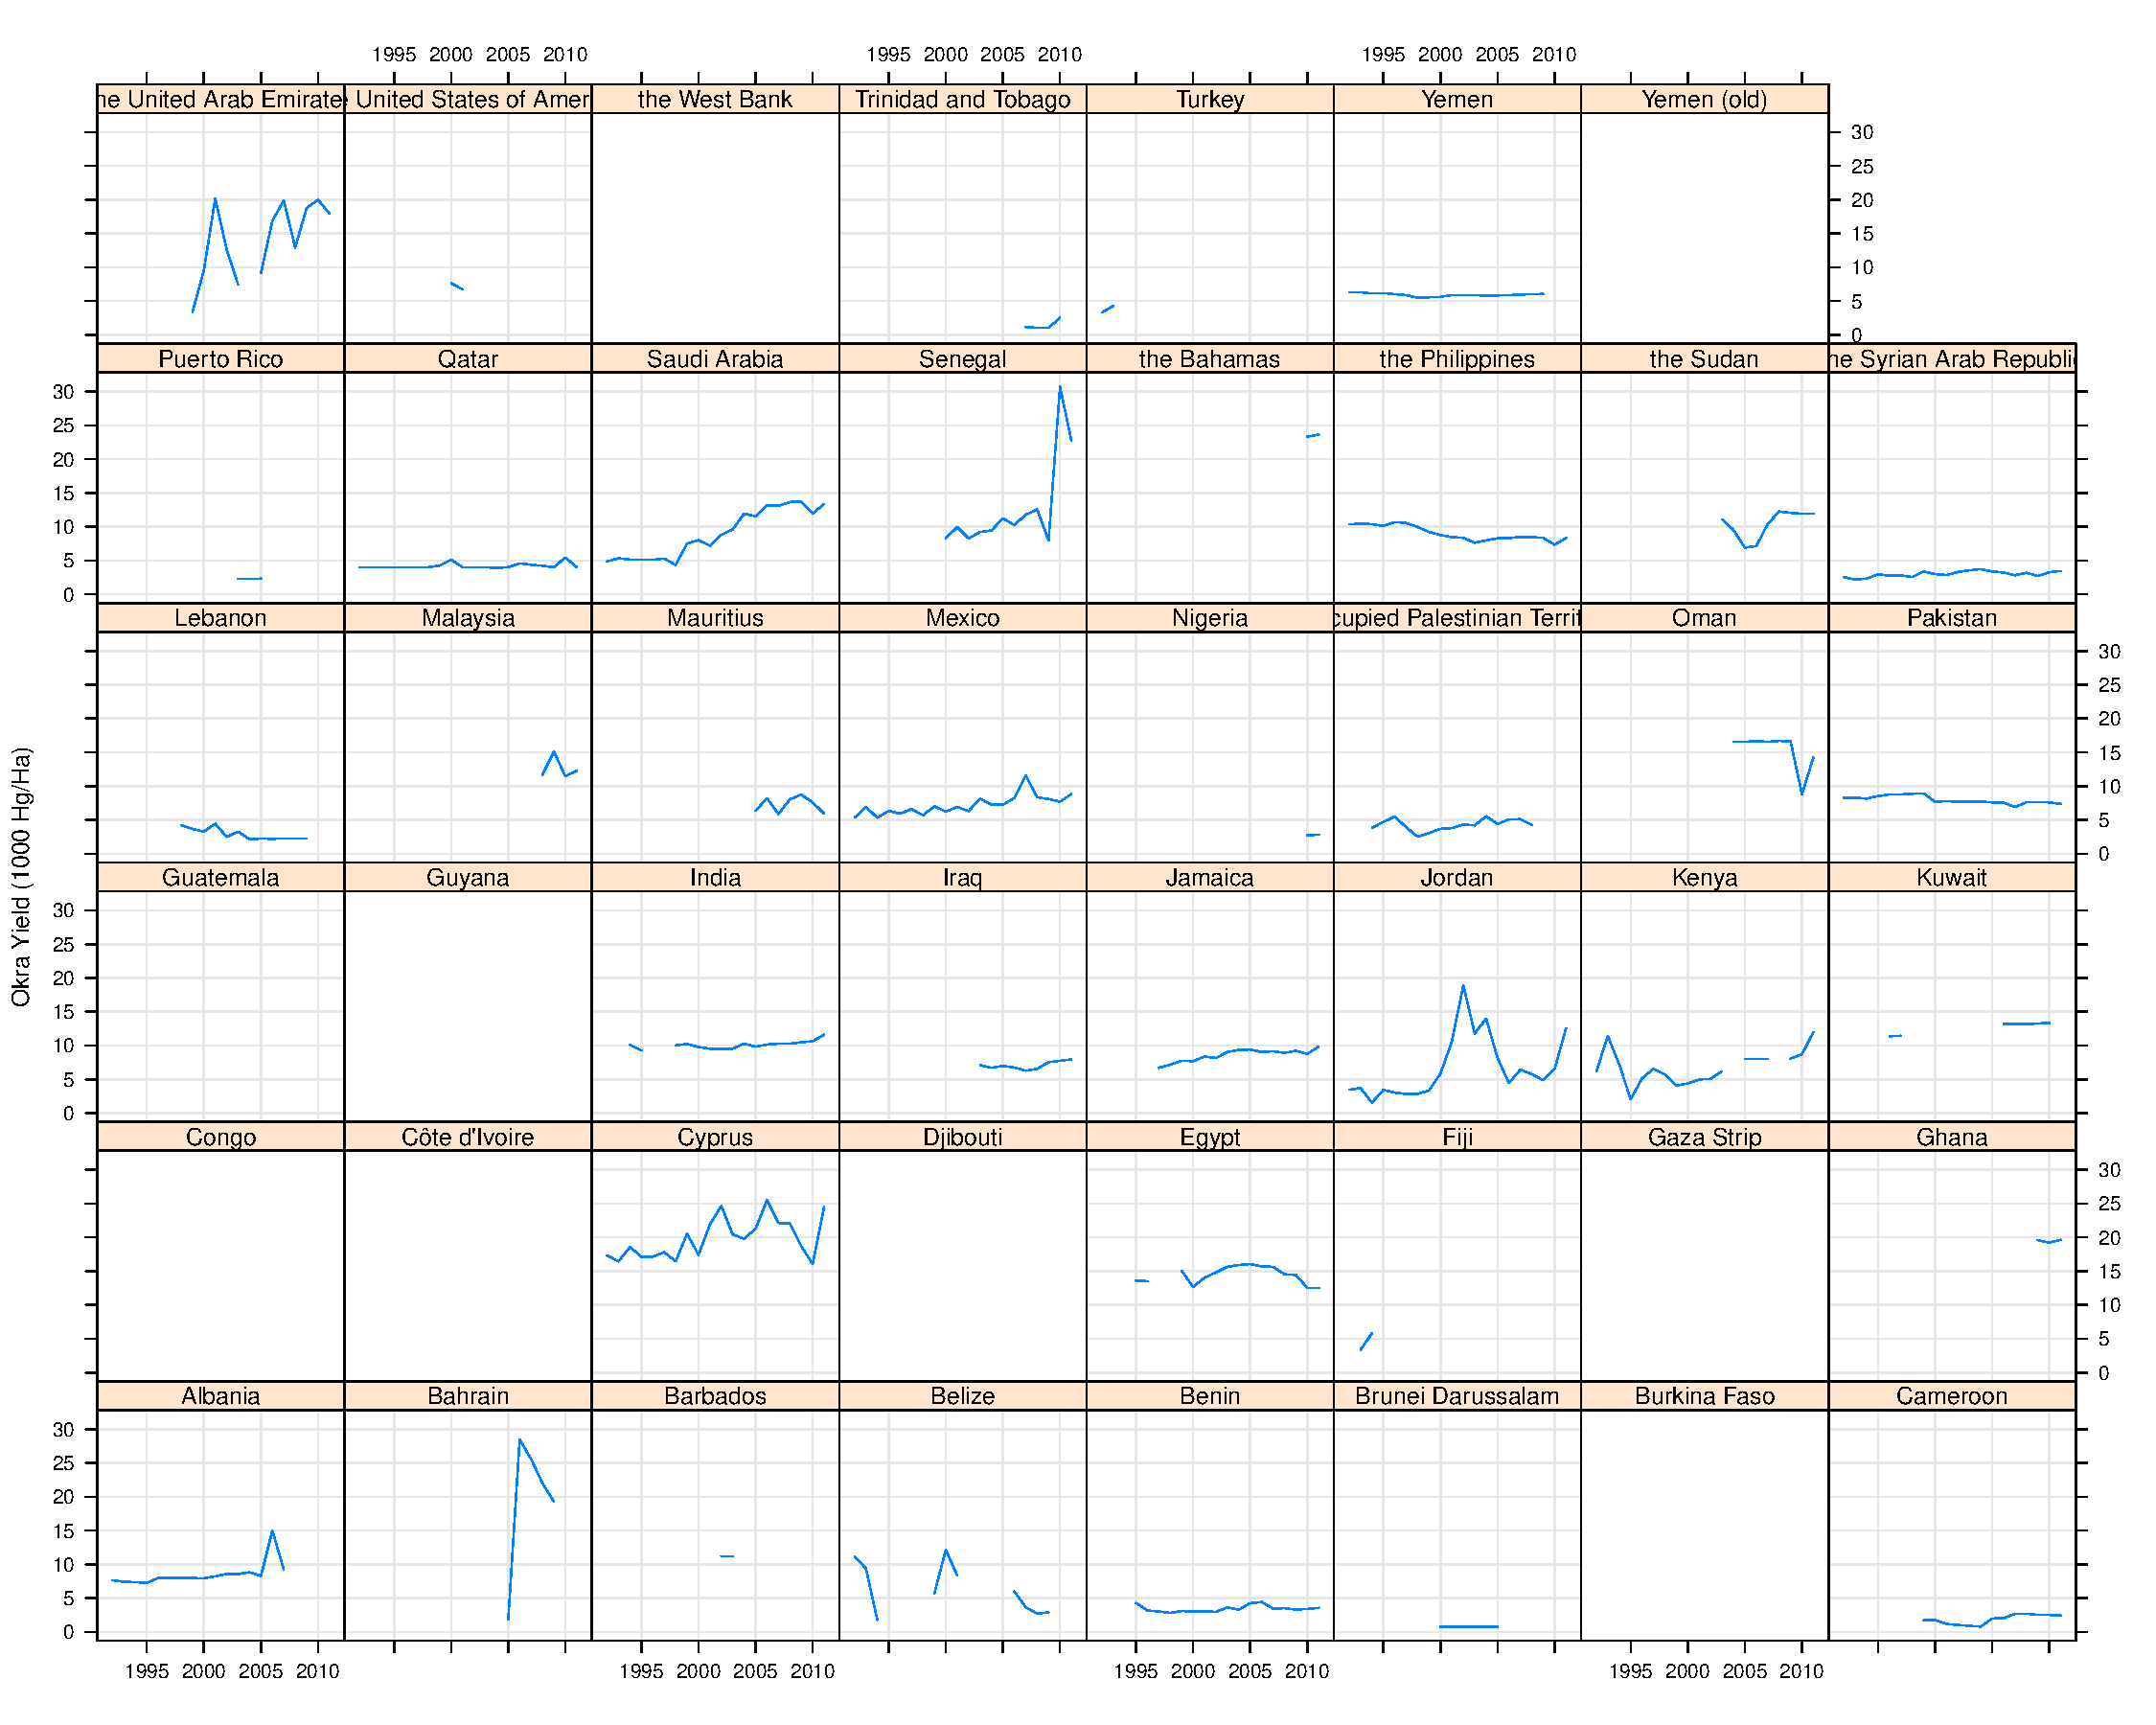
\includegraphics[width=\maxwidth]{figure/okra-yield-explore} 

}

\caption[Shown in this graph are the yield of Okra over time]{Shown in this graph are the yield of Okra over time. We can observe that the data is extremely sparse, further the quality of the data is questionable. Yield growth from less than 10 Hg/Ha to greater than 30 Hg/Ha in a single year for both Bahrain and Senegal is deemed suspicious.\label{fig:okra-yield-explore}}
\end{figure}


\end{knitrout}


\begin{knitrout}
\definecolor{shadecolor}{rgb}{0.969, 0.969, 0.969}\color{fgcolor}\begin{figure}[!ht]


{\centering 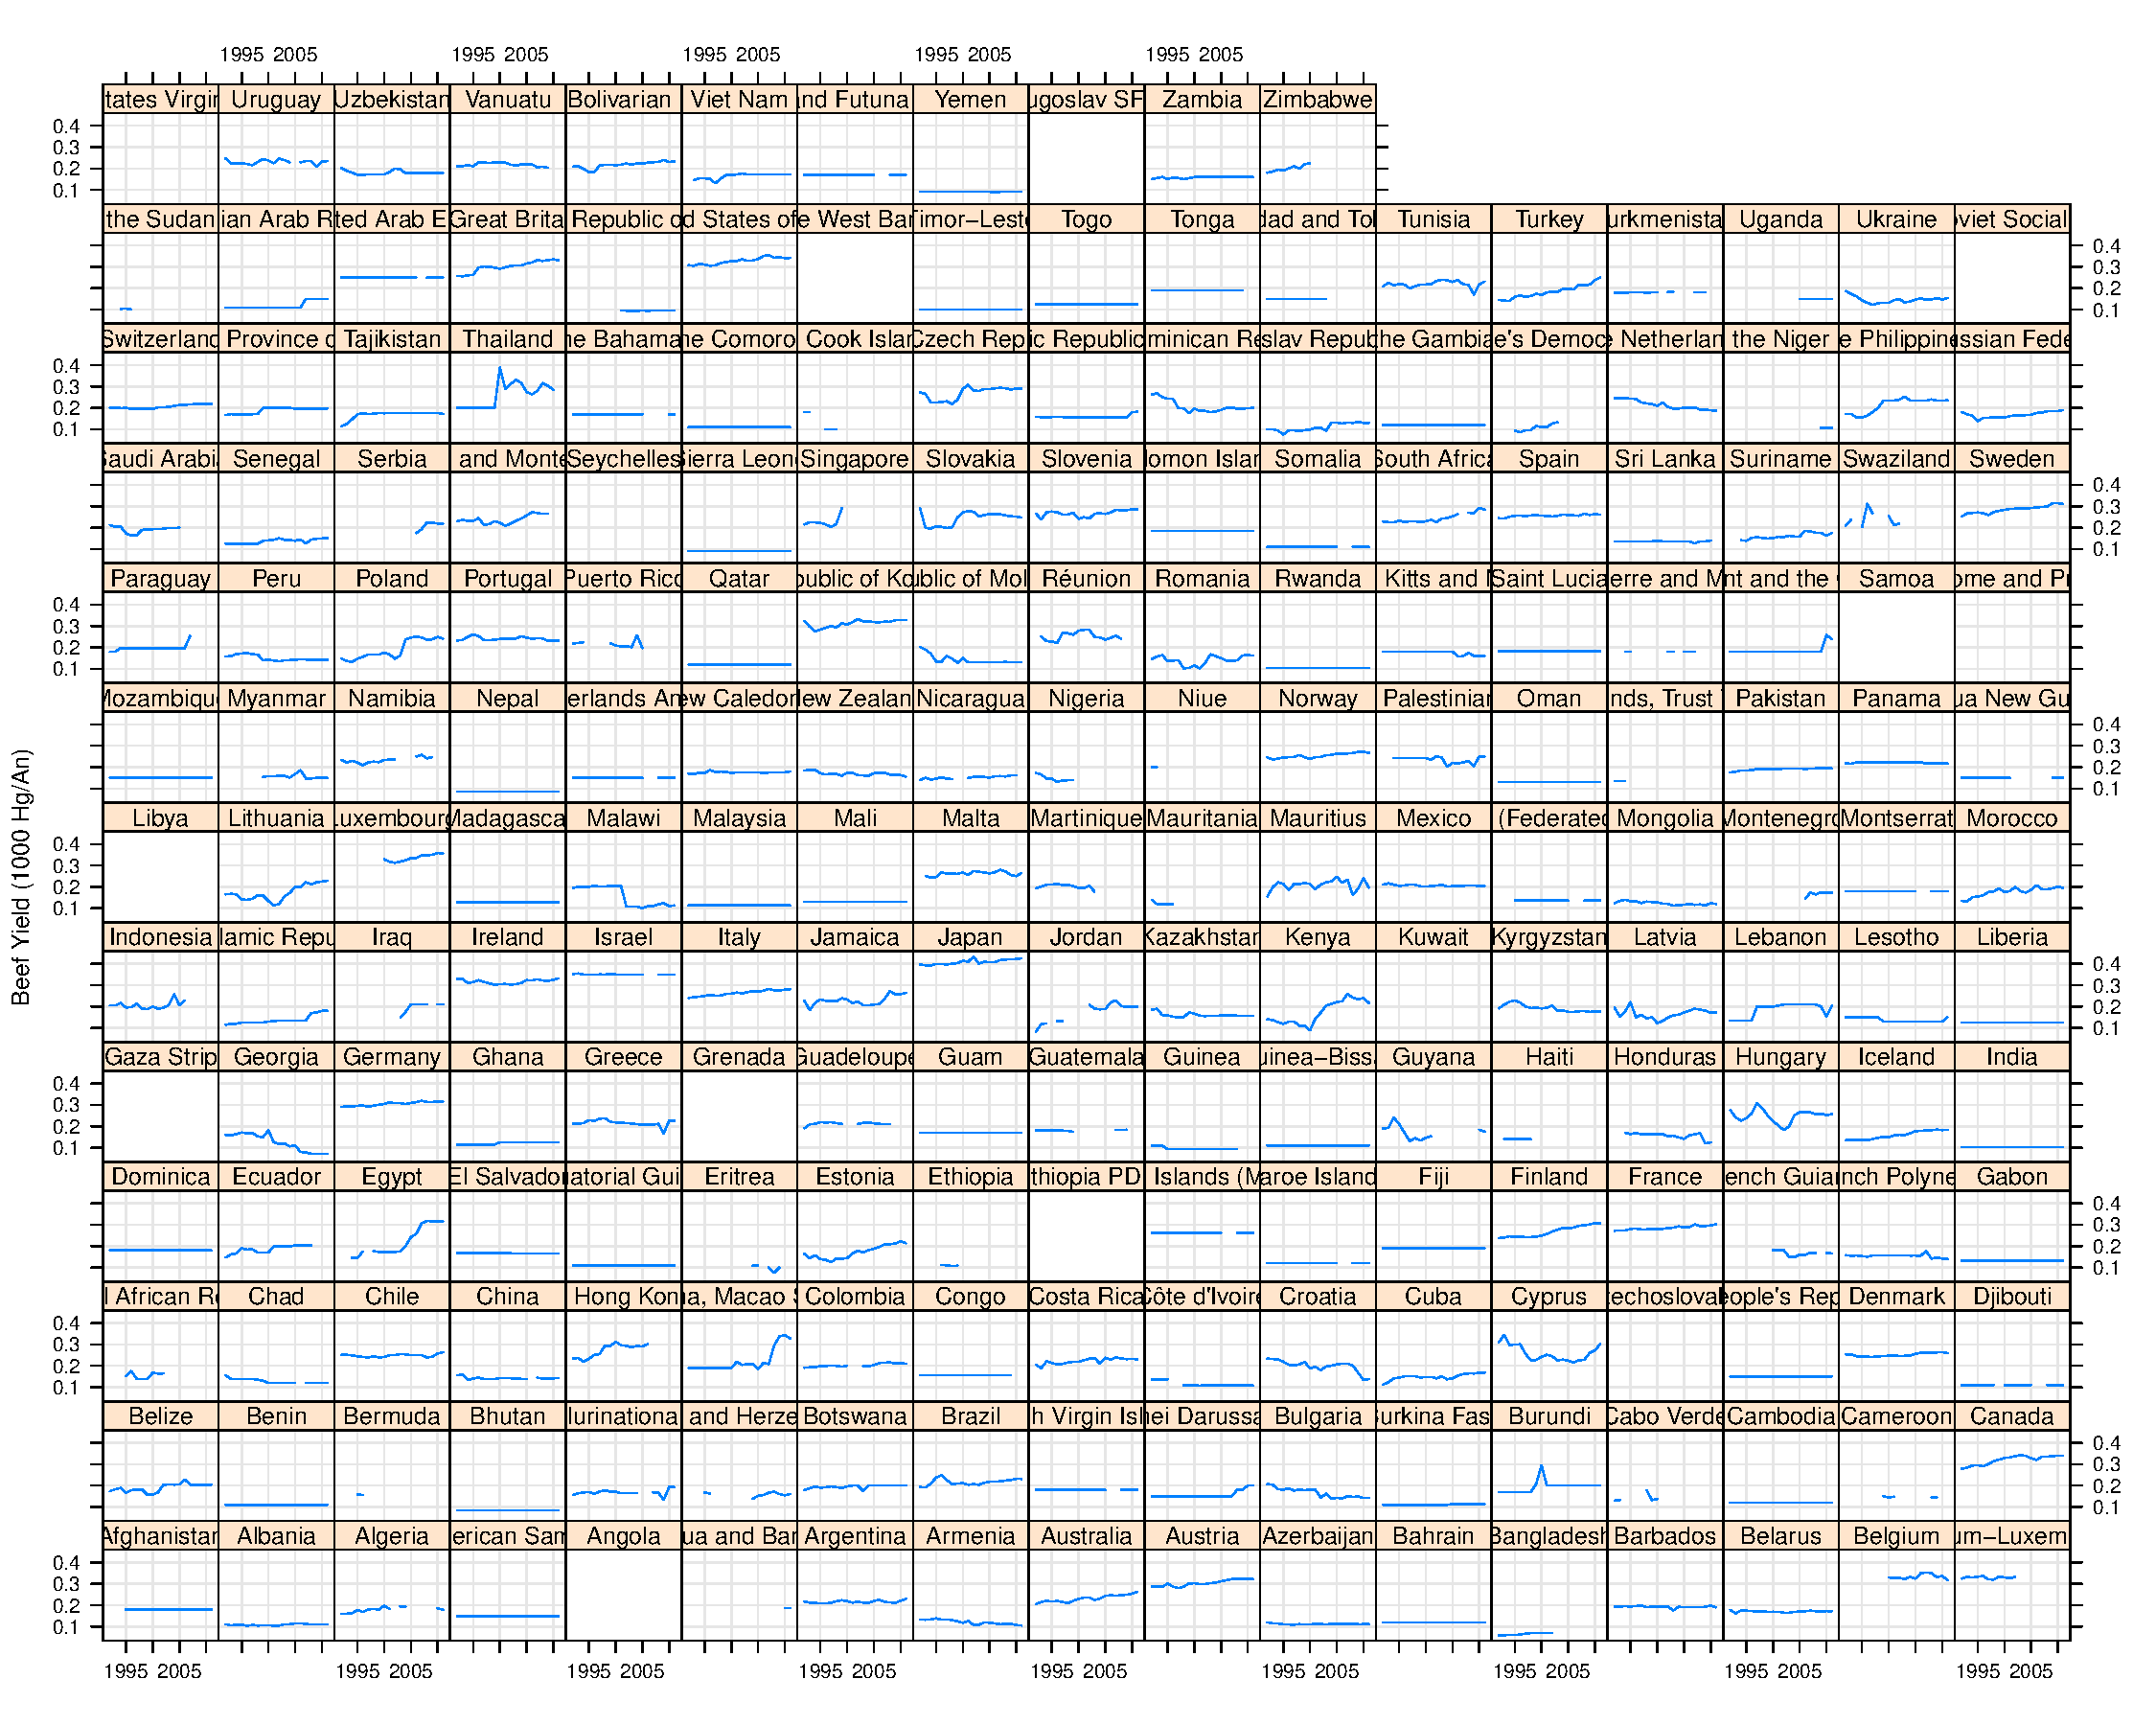
\includegraphics[width=\maxwidth]{figure/beef-yield-explore} 

}

\caption[Similar to grape, the carcass weight per animal of beef also shows the same pattern of a very modest improvement in yield with a handful of exceptions]{Similar to grape, the carcass weight per animal of beef also shows the same pattern of a very modest improvement in yield with a handful of exceptions.\label{fig:beef-yield-explore}}
\end{figure}


\end{knitrout}




\FloatBarrier
\subsection{Production and Area Harvested}

Although yield plays a vital role in the production process, the
actual quantity of production is usually dictated by the area sown and
harvested. The illustrations in this section shows that the production
series is usually dominated by how much area was planted and
harvested.\\

In contrast to the simple mechanism of yield where all dominant
factors contribute towards improving the productivity, the mechanism
of production is much more unpredictable. \\

Production is determine by area harvested and hence area sown in the
previous period by the farmer. Which ultimately depends on the
perception of information and subjective judgement of the
producer. Production can increase or decrease production as a response
to the state of the market, wheat field can be substitue to harvest
sorghum if prices are expected to be high. Further, individual
entities faces different risk profile, even under the assumption of
all producers are profit-seeking the risk profile may alter the
portfolio of products held by the producer. Markets has been known to
be difficult to forecast, let alone the prediction of human judgement
is just shy of impossible under curren state of understanding.\\

Only in cases where the commodity is a major staple or exporting item,
we can observe simple trend explained by the continuous increase in
demand. On the other hand, commodities which are of relative lesser
importance, the pattern of the production may display unpredictable
erratic behaviour.\\



\begin{knitrout}
\definecolor{shadecolor}{rgb}{0.969, 0.969, 0.969}\color{fgcolor}\begin{figure}[!ht]


{\centering 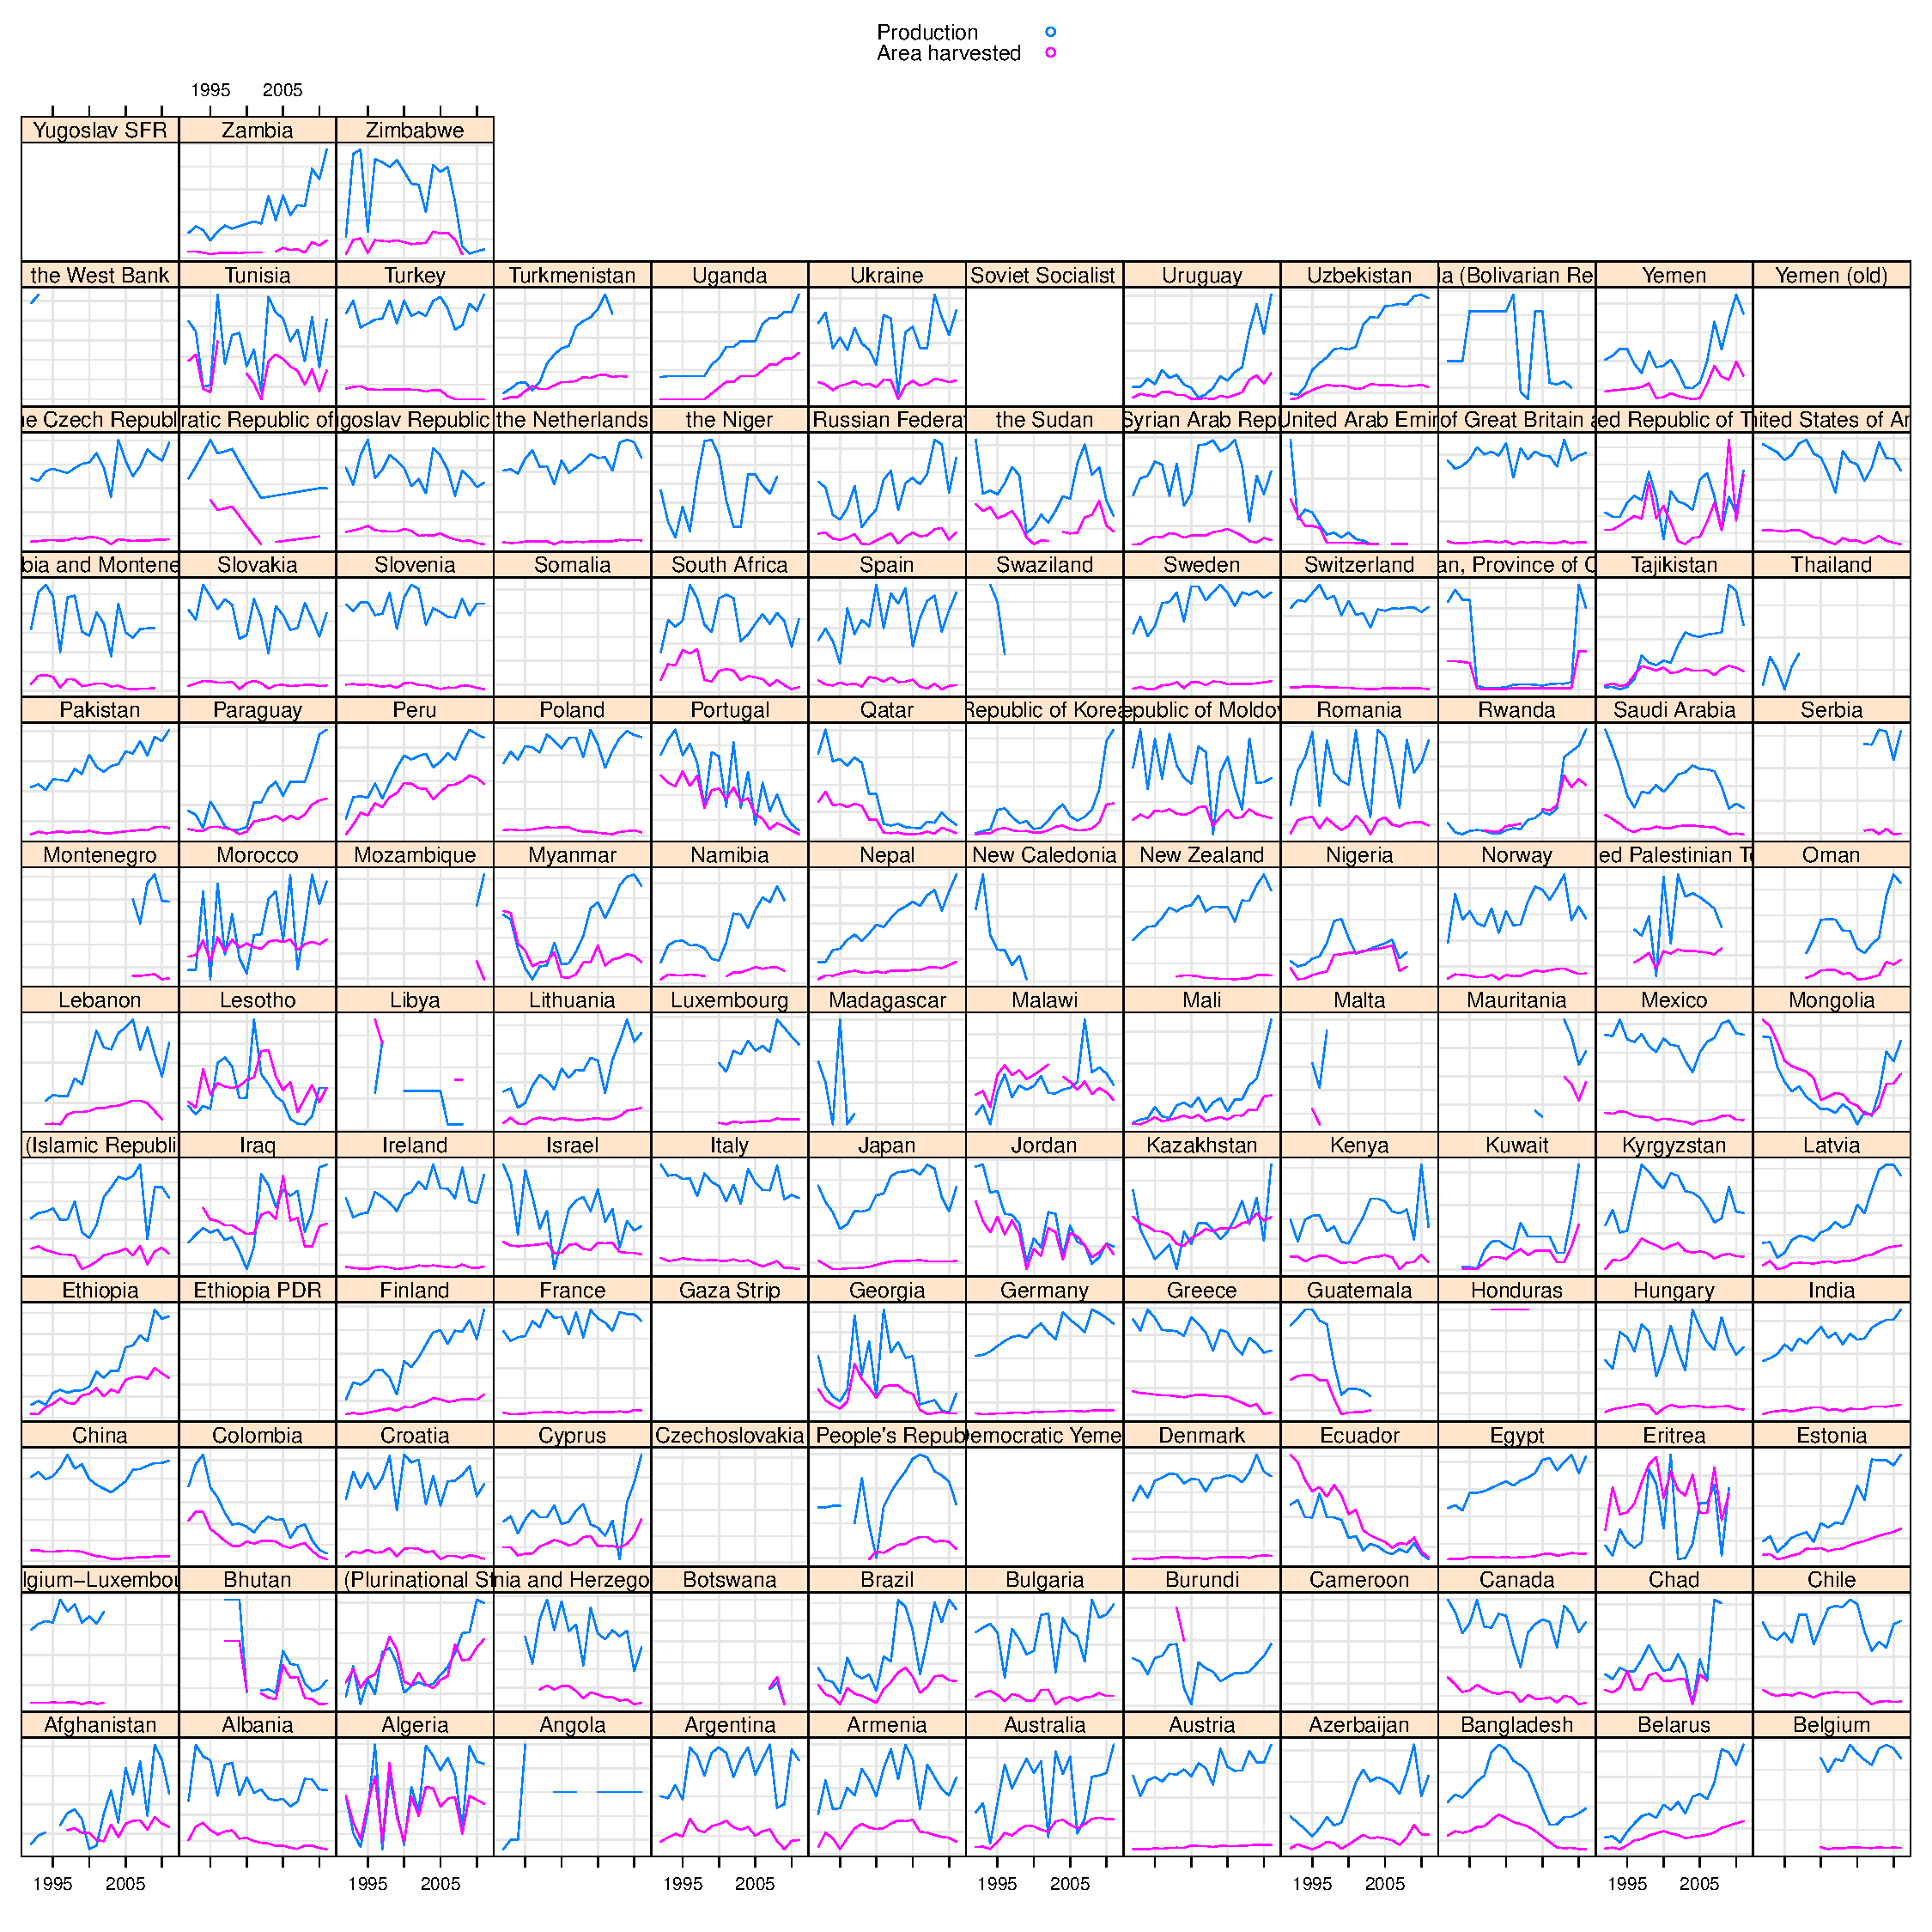
\includegraphics[width=\maxwidth]{figure/wheat-production-area-explore} 

}

\caption[Wheat production and area harvested by country]{Wheat production and area harvested by country. The figure shows that excluding several producers such as India, Nepal, and Pakistan which has a stable trend in production, both the production and area of most countries display erratic behavior.\label{fig:wheat-production-area-explore}}
\end{figure}


\end{knitrout}




\begin{knitrout}
\definecolor{shadecolor}{rgb}{0.969, 0.969, 0.969}\color{fgcolor}\begin{figure}[!ht]


{\centering 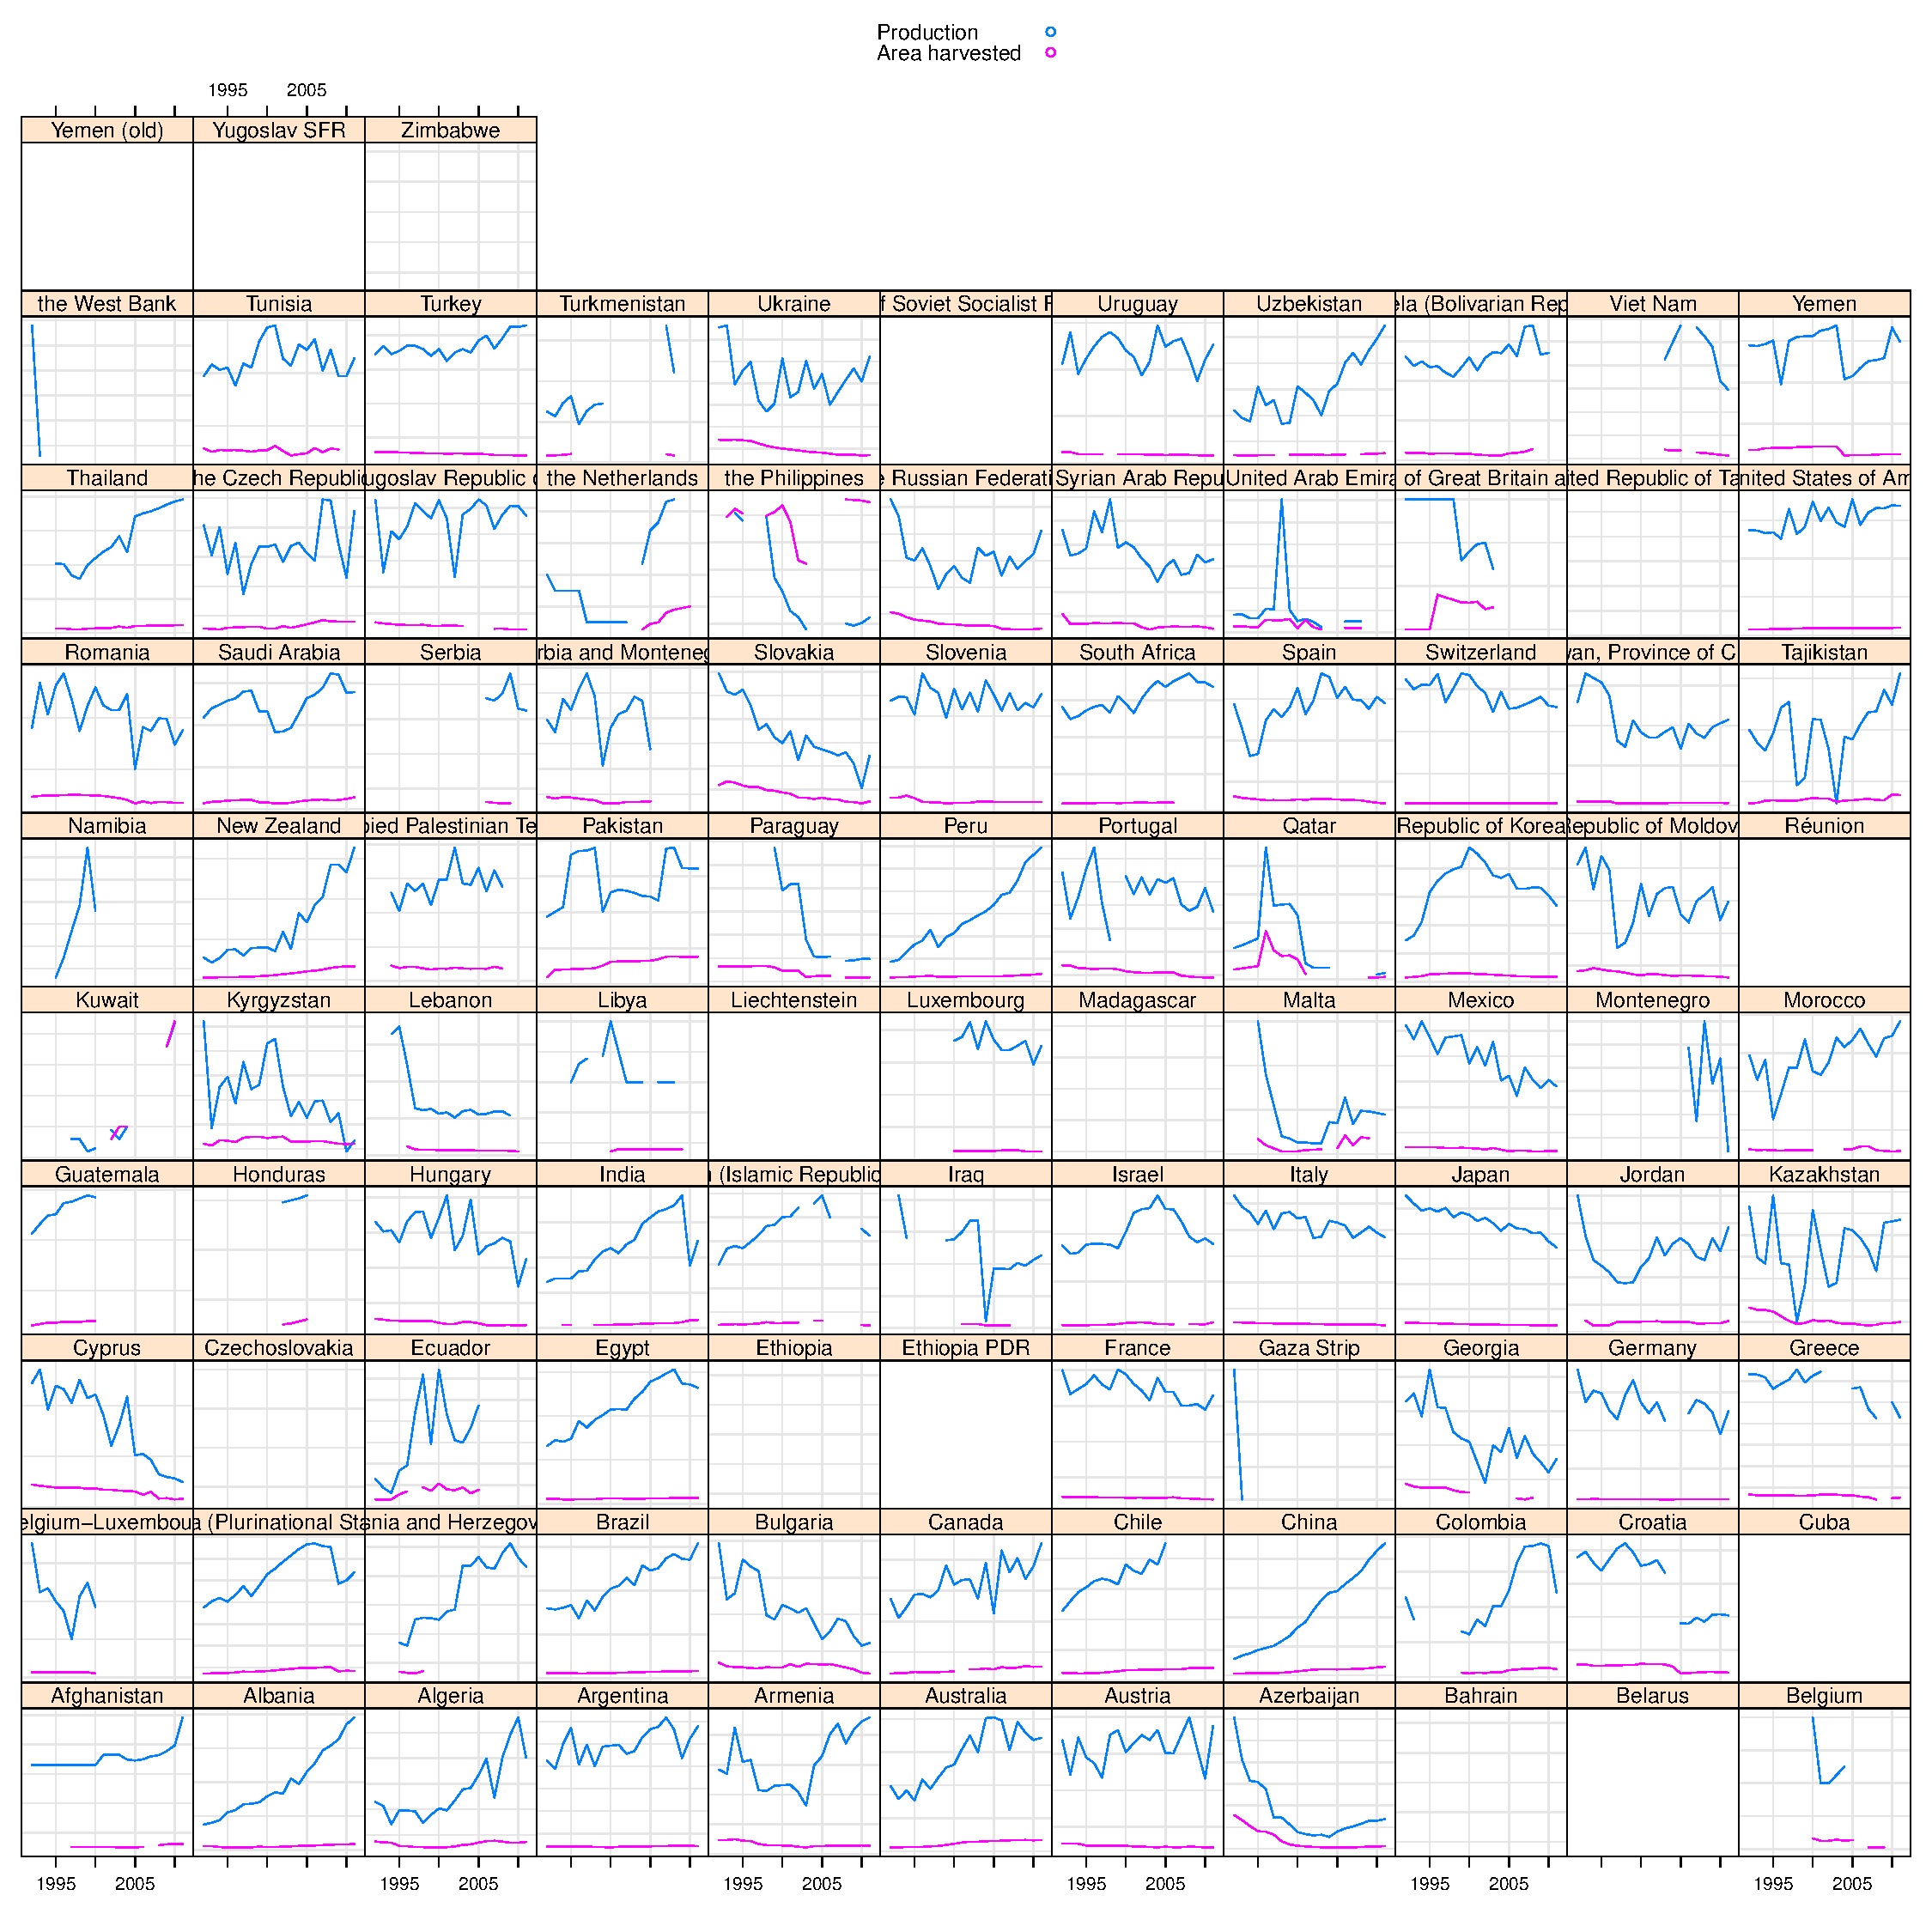
\includegraphics[width=\maxwidth]{figure/grape-production-area-explore} 

}

\caption[In contrast to wheat, the area for grape is much more stable, a character of tree which takes year to plant and nuture and the alteration of the land use is much more difficult]{In contrast to wheat, the area for grape is much more stable, a character of tree which takes year to plant and nuture and the alteration of the land use is much more difficult. Nonetheless, the production also display different trends over different time period\label{fig:grape-production-area-explore}}
\end{figure}


\end{knitrout}

\begin{knitrout}
\definecolor{shadecolor}{rgb}{0.969, 0.969, 0.969}\color{fgcolor}\begin{figure}[!ht]


{\centering 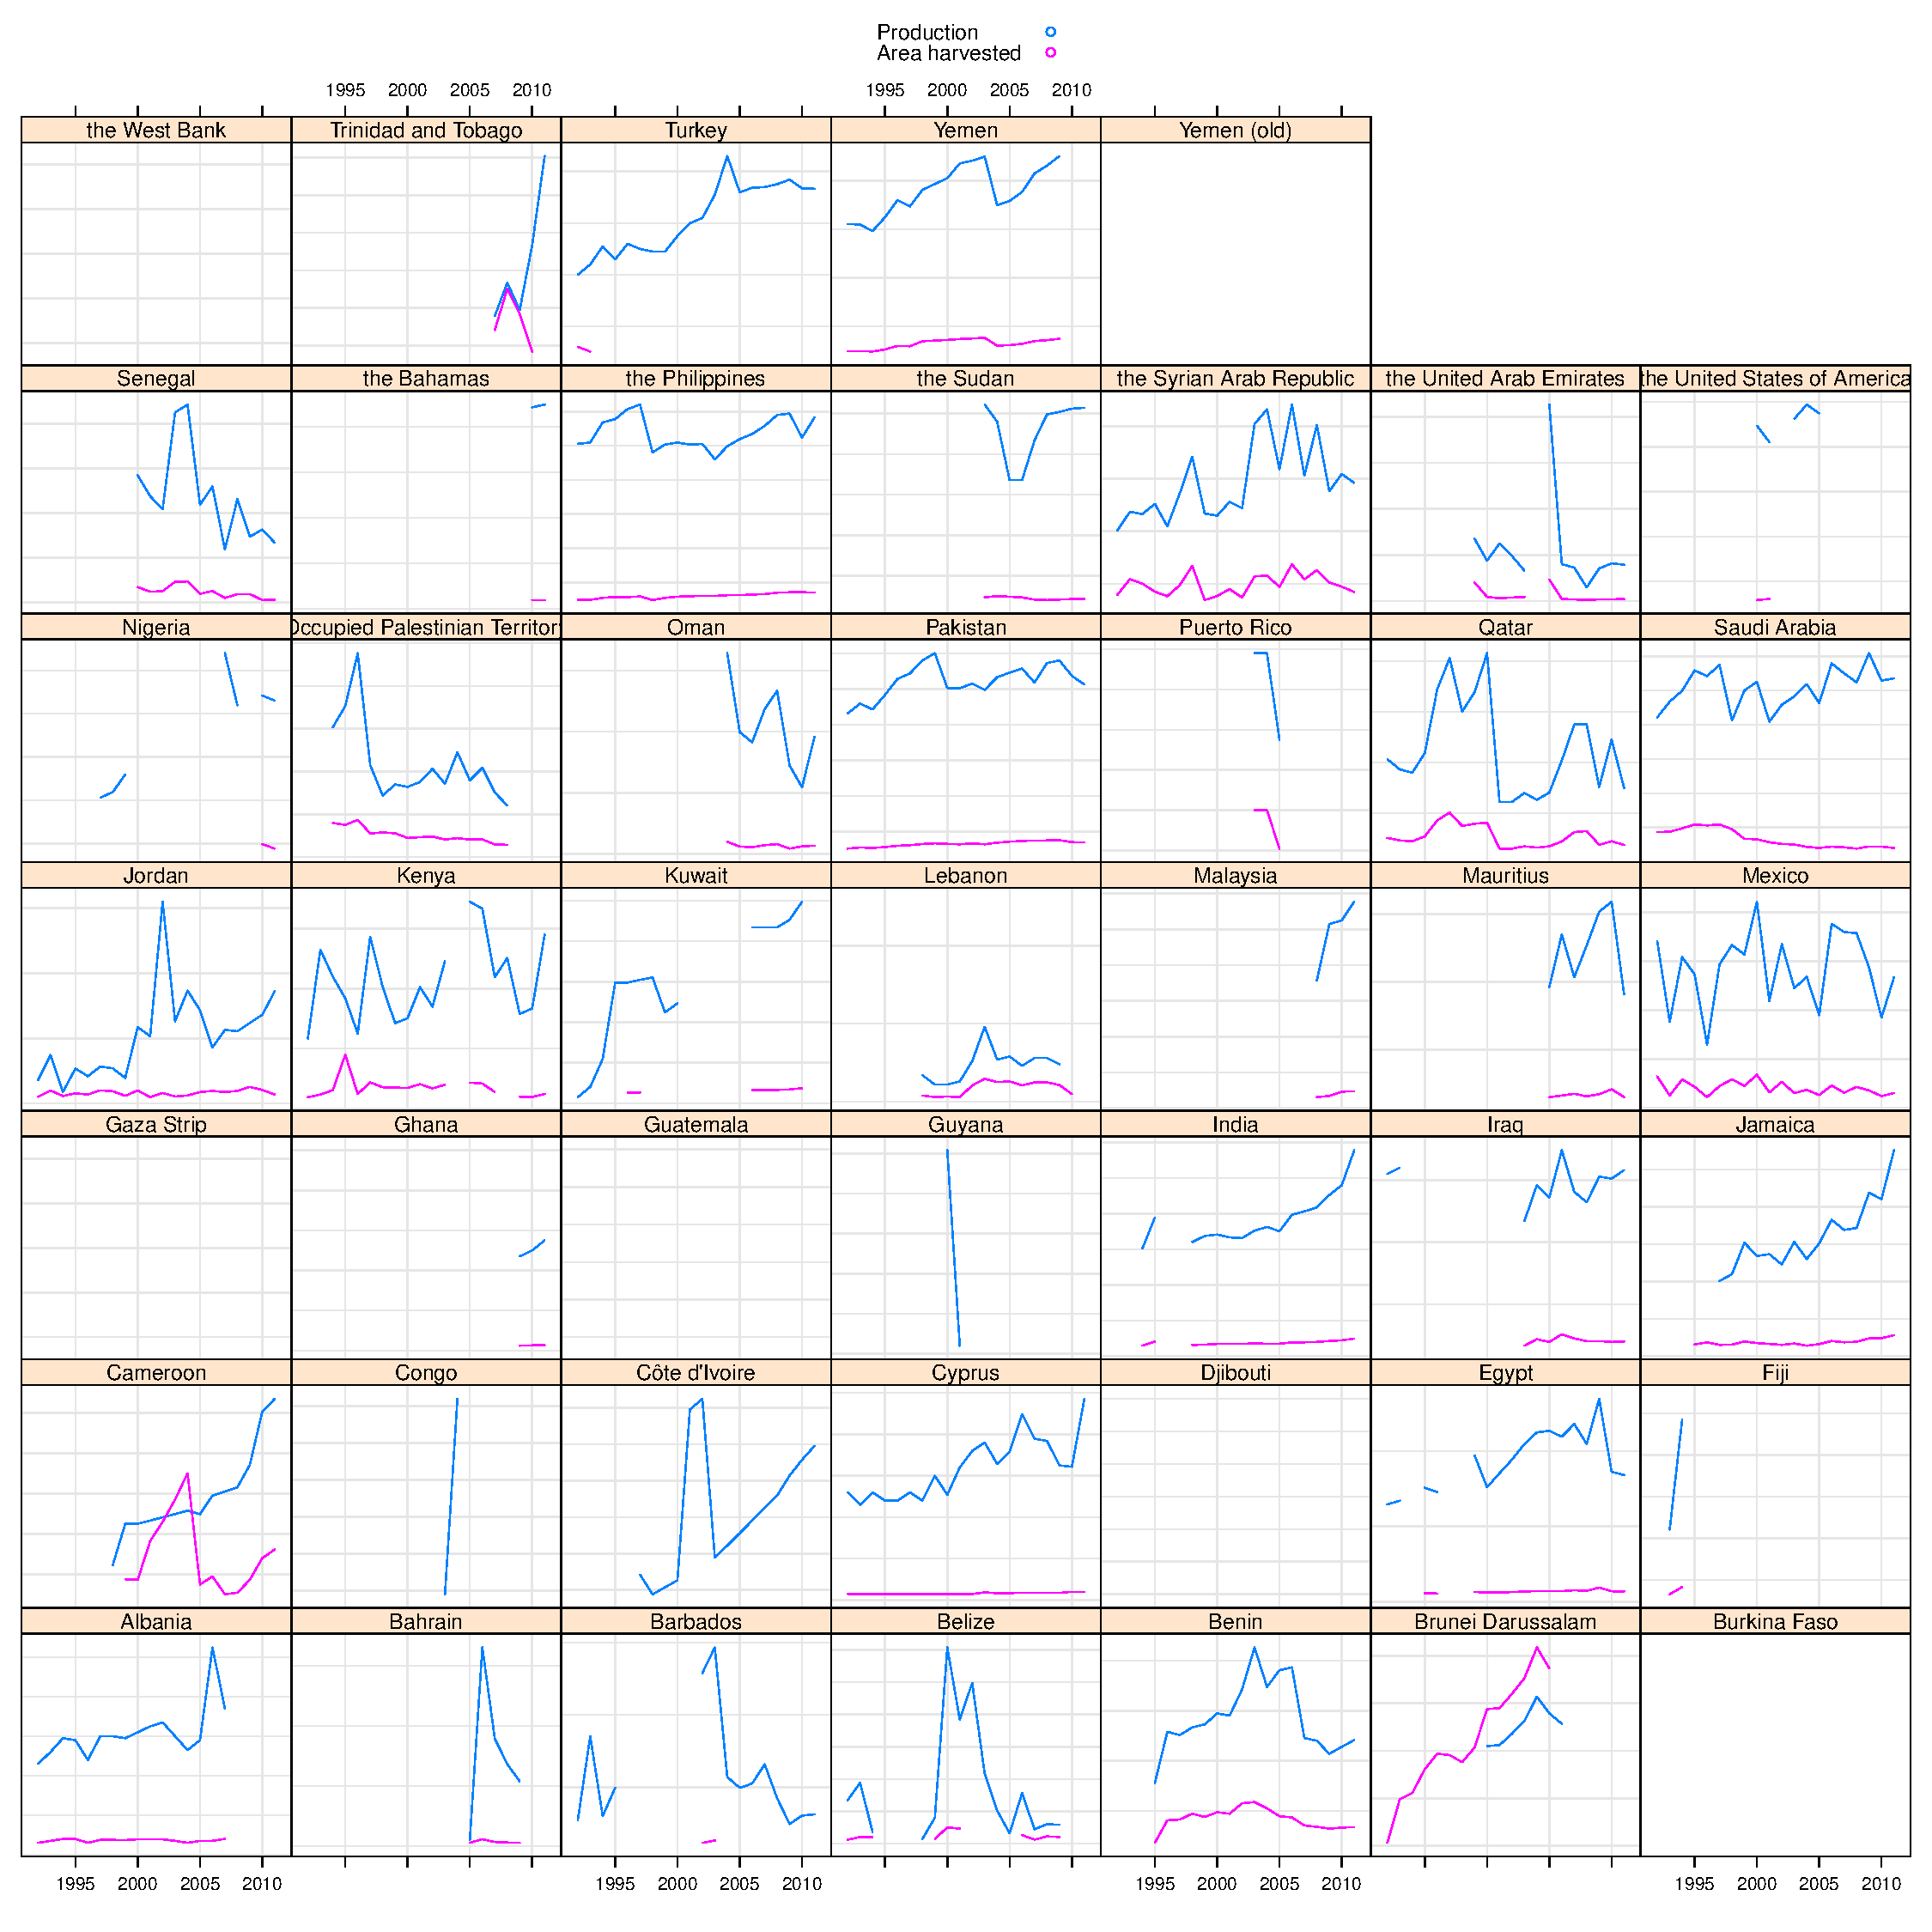
\includegraphics[width=\maxwidth]{figure/okra-production-area-explore} 

}

\caption[Even more so than both wheat and grape, the production of okra appears to demonstrate unpredictable trends and shocks]{Even more so than both wheat and grape, the production of okra appears to demonstrate unpredictable trends and shocks.\label{fig:okra-production-area-explore}}
\end{figure}


\end{knitrout}

\begin{knitrout}
\definecolor{shadecolor}{rgb}{0.969, 0.969, 0.969}\color{fgcolor}\begin{figure}[!ht]


{\centering 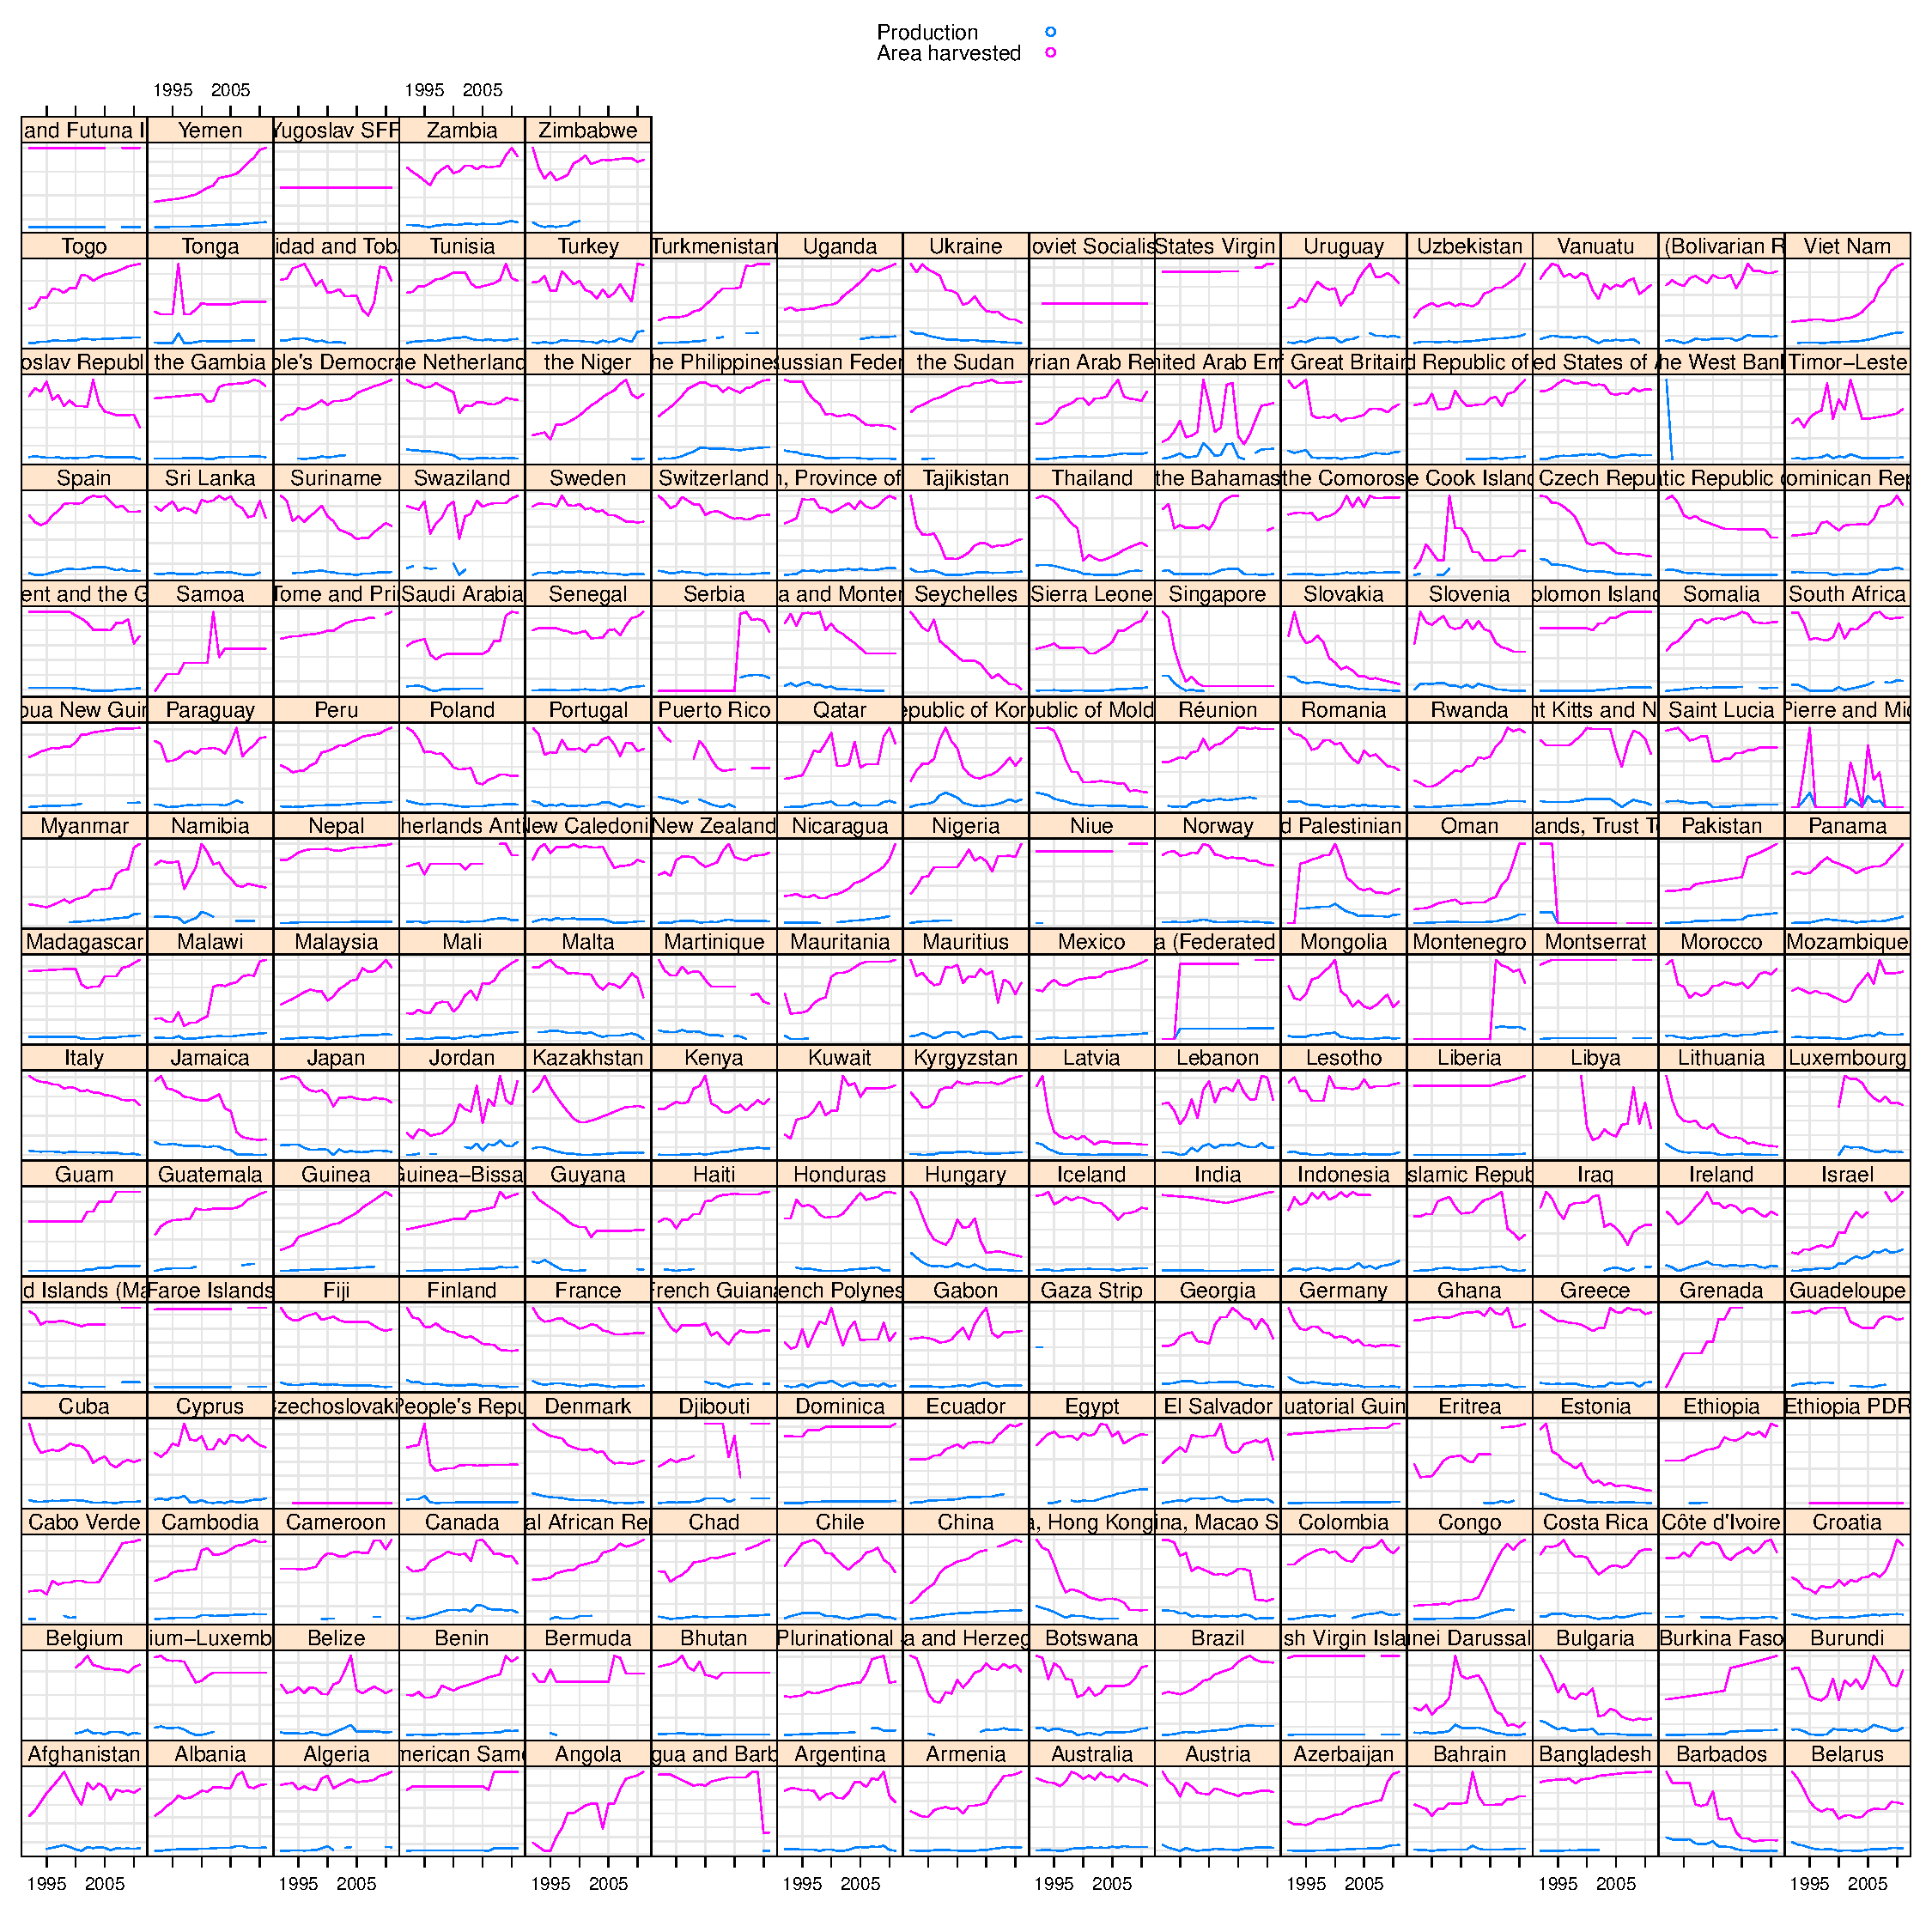
\includegraphics[width=\maxwidth]{figure/beef-production-area-explore} 

}

\caption[Of all the production, livestock meat such as beef and veal may have been the easiest to predict and impute]{Of all the production, livestock meat such as beef and veal may have been the easiest to predict and impute. There is continuing demand around the world for meat, while shift in production is usually difficult due to the high expenditure in machinery capital. With this being said, we can likewise observe shocks and or period of contraction or expansion over time.\label{fig:beef-production-area-explore}}
\end{figure}


\end{knitrout}


%% One worthnoting point is that production which display simple pattern
%% are typically commodities in countries which are highly commercialized
%% or important for consumption as staple or traded for financial
%% resources. These item are rarely the one we need to impute as they are
%% generally complete, it is commodities of lesser importance that are
%% required to be imputed and as a result that are often harder due to
%% their unstable demand and nature.\\


\FloatBarrier
\subsection{Data Quality Issues}
During the development of the methodology, we have encountered several
data quality issues which required us to review and redefine our
initial methodology. These are not exceptions, rather they are
prevalent in the production domain and the analyst should bear in mind
of these characteristics.


\subsubsection{Extremely High Sparsity}
Although missing values are expected provided the goal of the task is
to impute missing values, but one may be stunned at the sparsity of
the data. For commodity such as pepper, merely 20\% of the data are
observed which raises the question whether imputation remain valid.

\subsubsection{Diverging Trends and shocks}
Another issue arose from the quality of the data reported and
recorded. It is not uncommon to observe unexplainable diverging trends
or shocks of production and area harvested which resulted in exploding
yield. The yield of Okra for Bahrain and Senegal in figure
\ref{fig:okra-yield-explore} are prime examples. Coconut production of
China in 2008 is another example, a change in classification resulted
in large escalation of production while the area harvested remained
similar to the previous year resulted in a three-fold increase in the
yield solely for that particular year.\\

\subsubsection{No indicator distinguish zero, missing values and not application}
The analyst should be made aware of the fact that although a framework
does exist to distinguish zero and missing values in the database, in
practice this may not be the case.\\


These observations prompt us to devise a robust method to safeguard
ourself from non-sensical imputation.\\



%% Furthermore, these observation are being reported back to the data
%% collection team to further improve the overall quality of the data.

\FloatBarrier
\section{Proposed Methodology}

In this section we will provide a detailed explanation of the proposed
methodology with illustration.



\subsection{Imputation for Yield}

The determination of yield can be categorise into three components, a
trend which reflects improvement in technoglogical innovation and
fluctuation as a result of climate related factors with adhoc events
such as war and diseases causing shocks to the series. \\


Climate effect can be broadly grouped into two category, year-to-year
variation and cyclical-catastrophical. Year-to-year changes in
temperature, precipitation will result in small variations around the
trend while cyclical-catastrophical phenomenon such El Ni\~{n}o will
appear as shocks. Both are difficult to employ in practice since data
such as temperature and precipitation suffer problem from period
matching; using annual data will reduce correlation and create
spurious noises, while monthly data will have to be matched crop by
crop by identify the relevant months corresponding to the production
cycle. \\

Shocks such as war or diseases are difficult to model due to
the number of events observed in the history is small and the effect
of each event may be different.

On the other hand, the continuous advacement of technology and
innovation and increasing productivity can be capture by a simple
smoothing trend.\\

The proposed methodology for imputing the yield is a linear mixed
model with splines, the utilization of this model enables all
information available both historical and cross-sectional to be
incorporated. This allows us to capture not only the technological
advancements in a specific commodity, but at the same time the
relative speed of technological adoption of the country. In addition,
proposed indicators such as the vegetation index, $\text{CO}_2$
concentration and other drivers can be tested and incorporated if
proven to improve predictive power.\\


\subsubsection{The model}
Following the notation of Bates, the general form of the model can be
expressed as:

\begin{align}
  (\mathscr{Y}|\mathscr{B} = \mathbf{b}) &\sim
  \mathscr{N}(\mathbf{X}\boldsymbol{\beta} + \mathbf{Z}\mathbf{b},
  \boldsymbol{\sigma^2}\mathbf{I})\nonumber \\
  \mathscr{B} &\sim\mathscr{N}(\mathbf{0}, \boldsymbol{\Sigma_\theta})
\end{align}

Where the fixed component $\mathbf{X}\mathscr{\beta}$ models the
effect of exogenous variables when supplied, while the random
component of $\mathbf{Z}\mathbf{b}$ captures the aggregated effect of
innovation and improved practice of each specific country and
commodity. \\

More specifically, the model implemented has the following expression:
\begin{align}
  \label{eq:lmeImpute}
  \text{Y}_{i,t} &= \overbrace{\beta_0 + \sum_{j=1}^{p}\beta_j x_j}^{\text{Fixed effect}} +
  \overbrace{b_{0} + \sum_{k=1}^{df}b_{k, i}B_{k}(t)}^{\text{Random effect}} +
  \epsilon_{i,t}
\end{align}

Where $Y$ denotes yield, $i$ for country, $t$ for time, and $k$ the
degree of freedom for the B-spline. The fixed effect is left for
external drivers such as precipitation and temperature.\\


To test the number of degree of freedom for spline required to capture
the presence of possible non-linearity, the algorithm proceed by
estimating the model with one degree of freedom then continue the
process by testing the hypothesis whether additional degree of freedom
is necessary.\\

Imputation is predictive in nature, therefore the test is designed to
select the model which provides optimal predictive performance. The
testing is performed by drawing bootstrapped samples and re-fitting
the model to obtain $b$ sets of prediction errors. Then we test
whether the newly proposed model has a lower out-of-sample prediction
error when compared to the benchmark model. The algorithm will test
iteratively until the proposed model has higher prediction error or
when the maximum degree of freedom specified has been reached.\\

\begin{gather*}
  H_0 : d\le0 ,\\
  H_1 : d>0 .\\
  \intertext{Where $d$ is defined as follow:}
  d = \sum_{b=1}^B\left(
  \frac{1}{N_1}\sum_{i=1}^{N_1}(\hat{Y}_{b, df} - Y)^2 - 
  \frac{1}{N_2}\sum_{i=1}^{N_2}(\hat{Y}_{b, df + 1} - Y)^2\right)
\end{gather*}

The B-splines implemented is first degree linear, from the exploratory
analysis we believe that higher order polynomial are not required. The
non-linearity can already be captured by having multiple degree of
freedom, increasing the order would only over-fit the data and can
display erratic imputation in the tails.\\


In essense, the imputation of the yield is based on the overall
country specific improvements in innovation while also capturing the
relative advancements in the designated commodity, both accross
time. Since more information are utilized and pooled together, imputed
values display stable characteristics while reflecting changes
resulting from different aspect.\\



\FloatBarrier
\subsection{Imputation for Production}

From the exploratory analysis, we can see that the trend and shape of
production and area harvested are closely related. Nonetheless, both
the series and missing mechanism can behave very different depending
on the country and the commodity. Furthermore, there does not seem to
be any readily usable information for us to model.\\


This is partly inherint in the nature of the size of the data which
compose vast variation of commodity and countries while at the same
time the relationship maybe too complex to be expressed in a suncinct
way. This is in contrast to the nature of yield where cross-country
and cross-commodity information can be pooled together for a better
informed imputation.\\

Land can be expanded or contracted between different commodities
depending on the price and expectation of the market, single block of
land can also be used for multiple commodity. Both market forces and
personal decisions are relatively unpredicatable which resulted in the
difficulty of imputation of area harvested and production.\\

This motivates us to employ what is known as ensemble learning to
impute the production and to deal with the multi-hypothesis
problem. \\

Given the strong correlation between area harvested and production, we
have decided to impute production and leave area harvested to balance.
This is based on expert advice that the production data are often much
more reliable and comprehensive.\\

In contrast to yield where all countries are imputed by a single model
to capture cross-country and cross-commodity effects; The production
imputation is performed country by country.\\

\subsubsection{The algorithm}
Ensemble learning in its simplest sense, is to build a collection of
simpler base models or learners which are later combine to obtain the
composite model or prediction. One of the most famous application was
the prediction of movie rating competition held by Netflix, which the
top two performer both used a form of ensemble. \\


The method consist of two steps:
\begin{enumerate}
  \item Building multiple models/learners.
  \item Combine the models or predictions.
\end{enumerate}


The ensemble method reduces the risk of choosing a poor model, this
resembles putting the eggs in different baskets. Thus we reduce the
risk of implementing a single model which may produce nonsensical
imputation for a certain subset of data. Moreover, model selection is
unecessary, since all model are included in the final ensemble.\\

Ensemble as described by Dietterich can mitigate the following
three issues.

\begin{itemize}
  \setlength{\itemindent}{1in}
  \item[\textbf{Statistical:}] Lack of data to identify an unique solution.
  \item[\textbf{Computational:}] Optimization
  \item[\textbf{Representational:}] Complex model
\end{itemize}



\begin{figure}[!ht]
  \centering
  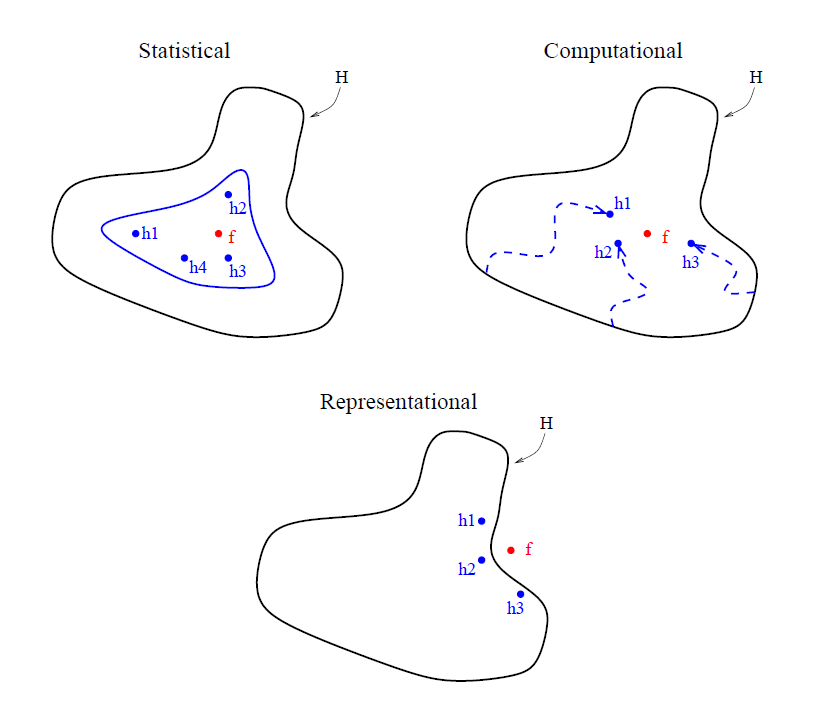
\includegraphics[scale = 0.7]{dietterich.png}
\end{figure}


The statistical problem refers to the lack of data to support a
particular hypothesis. The problem can be formulated as finding the
best hypothesis among competing models in the space
$\mathbf{\mathcal{H}}$. In the top left graph of the following
depicion from Dietterich we can see that hypothesis within the blue
boundary will give the same fit, and there is insufficient information
to determine which one is better. By combining the models, we may
reduce the risk of choosing a terrible model. If we only observe two
data points for a country, then fitting a linear line or a log curve
can both give the same fit and we may have no information to
distinguish the two.\\

The second problem which is lesser of an issue for our task is the
computational problem which applies to model which employs greedy
algorithm such as step-wise regression and classification tree. The
search within the hypothesis space at each step is local and thus has
a high probability of failing to achieve global maximum.\\

The final problem, representational, refers to the fact that the true
function $f$ can not be represented by any of the model. However, by
combining the models we may expand the space of representable
functions and potentially approximate the true function $f$ if it
exist. Take the production of beef in Oman and Vietnam for example, if
the production of a country has been growing at a linear rate in the
past, but expands rapidly in recent time, neither linear or
exponential model will provide a satisfactory result. However, an
ensemble combining a linear and exponential model will provide a good
solution by capturing different characteristics of the data.\\

From an integration point of view, the algorithm is adaptive in the
sense that if the data generating mechanism changes in the future, the
method will shift weights to models which better present the data and
thus reducing the need of constant monitoring and updating of
methodologies.\\

The model can also be seen as a mixture of different
expectations. From prior discussion, we know that the area and
production depends on the perception and cognition of information
leading to optimal judgement. However, even the same information can
lead to various decision as the information can be interpreted
differently and the model attempts to capture the difference in the
judgement by combining various expectation.\\



\FloatBarrier


The details of the ensemble implemented is describe here, the base
learner are listed in increaseing order of complexity. An effective
ensemble will have base models as diverse as possible. If there are no
diversity and all model generates similar result, then a correction
and the variance reduction property of the ensemble model will be
poor. The component chosen here range from no parameter global fitting
to flexible model which can capture local behaviours.\\

\begin{itemize}
  \item {\textbf{Base learners:}}
    \begin{itemize}
      \setlength{\leftmargini}{5em}
      \item[Mean:] Mean of all observations
      \item [Linear:] Linear Regression
      \item [Exponential:] Exponential function
      \item [Logistic:] Logistic function        
      \item [Naive:] Linear interpolation followed by last observation
        carried forward and backward.
      \item [ARIMA:] Autoregressive Integrated Moving Average model
        selected based on the AICC, and imputation via Kalman Filter.
      \item [LOESS:] Local regression with first degree local
        polynomial and sample size variant window.
      \item [Splines:] Cubic spline interpolation.
      \item [MARS:] Multivariate Adaptive Regression Spline
    \end{itemize}
  \item {\textbf{Combiner:}}
    non-trainable algebraic combiner - Weighted sum rule

    %% Type I: Standard
    \begin{align}
      p_n(x) &= \sum_{i=1}^K w_i f_{n, i}(x) \nonumber \\
      w_i &= \frac{\sum_{i = 1}^N(1/|f_{n, i}(x) - x|)^2}{\sum_{K}\sum_{i=1}^n(1/|f_{n, i}(x) - x|)^2}\nonumber
    \end{align}
    
    %% Type II: Shrinkage
    %% \begin{equation}
    %%   u_j(x) = \sum_{i=1}^N w_i f_{n, j}(x) \qquad w_i = 0 \quad
    %%   \text{if} \quad d_{n,j}(x) < k \nonumber
    %% \end{equation}
    
\end{itemize}

Where the weights ($w_i$) of model $i$ depends on the corresponding
fit ($f_{n, i}(x)$) on the available data with a ceiling set at
70\%. The naive imputation which does not have a fitted model always
take uniform weights. A much more favourable method is to compute
weights based on the prediction error obtained from bootstrap or
jackknife, yet the missing values restrict us to draw any reasonable
size for sub-sample fitting. This is further penalized by the time
series nature of the data where boostrap with replacement is not
possible.\\

In this section, we take a sample of production from the exploratory
analysis section and illustrate the imputation methodology. The
selection of the sample is intended to illustrate the flexibility and
robustness of the methodology, rather than based on the importance nor
the quantity of the product.\\

The black points in the graph represents observed data while the
thicker blue line represents the final ensemble model with the points
being the estimation of missing values. Other lines represents the fit
of the component models, the weight of each model is displayed in the
legend.\\

Component models which failed to fit the data has a weight of 0.\\

\begin{knitrout}
\definecolor{shadecolor}{rgb}{0.969, 0.969, 0.969}\color{fgcolor}\begin{figure}[!ht]


{\centering 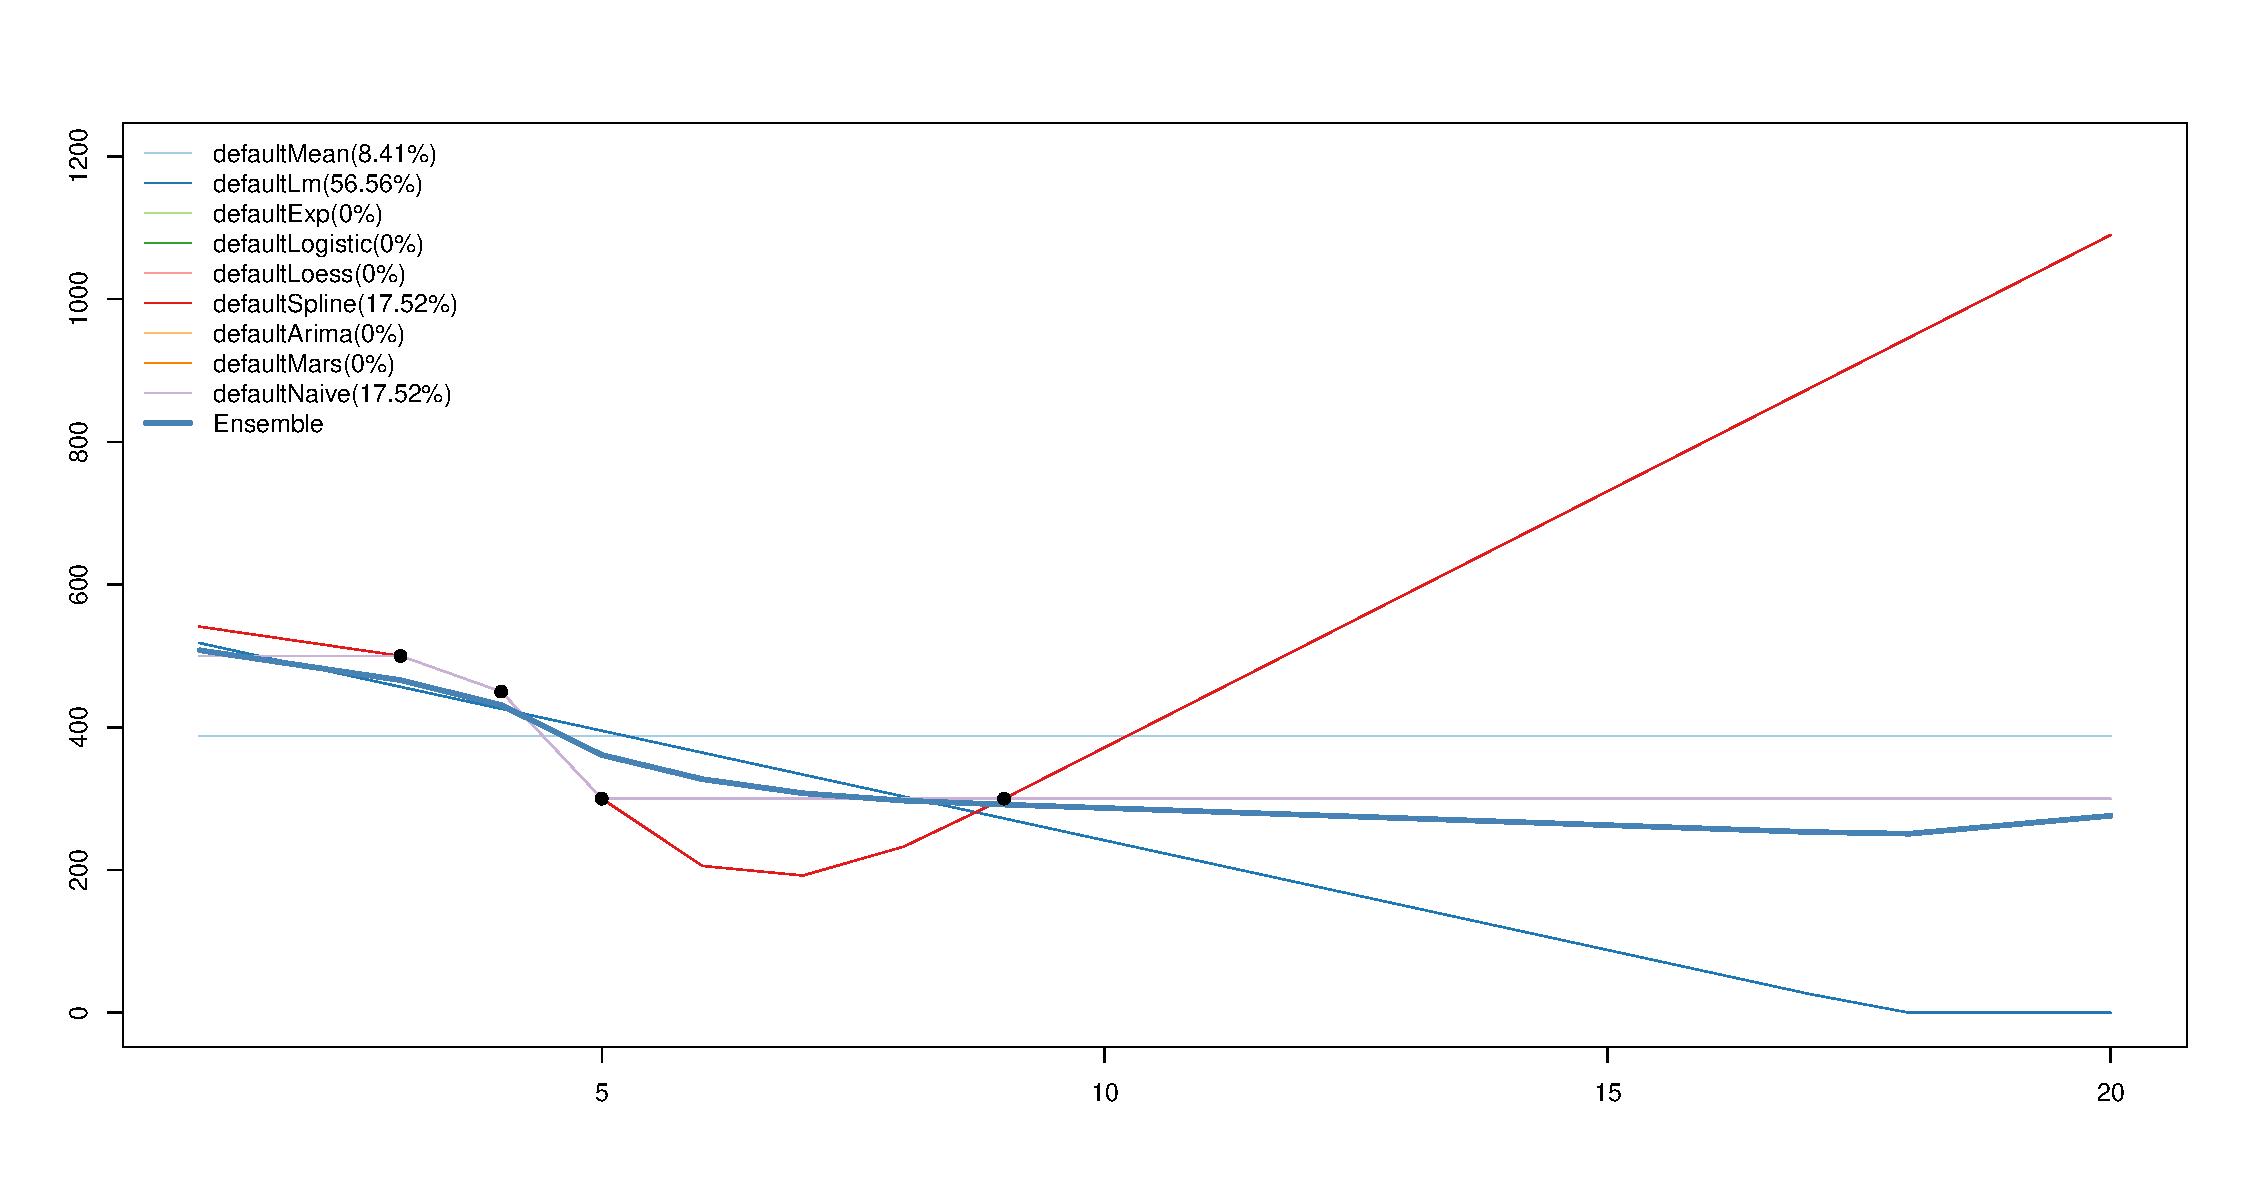
\includegraphics[width=\maxwidth]{figure/wheat-swaziland-impute} 

}

\caption[This selected series is the production of wheat in Swaziland, from the black observed production we can see that no data has been observed in the paste 10 years]{This selected series is the production of wheat in Swaziland, from the black observed production we can see that no data has been observed in the paste 10 years. Yet, the ensemble fits several possible extrapolation which all seem reasonable. Yet, we can see that although the linear regression obtained the highest weight the ensemble is safe guarded by naive imputation and spline so it does not go below zero.\label{fig:wheat-swaziland-impute}}
\end{figure}


\end{knitrout}

\begin{knitrout}
\definecolor{shadecolor}{rgb}{0.969, 0.969, 0.969}\color{fgcolor}\begin{figure}[!ht]


{\centering 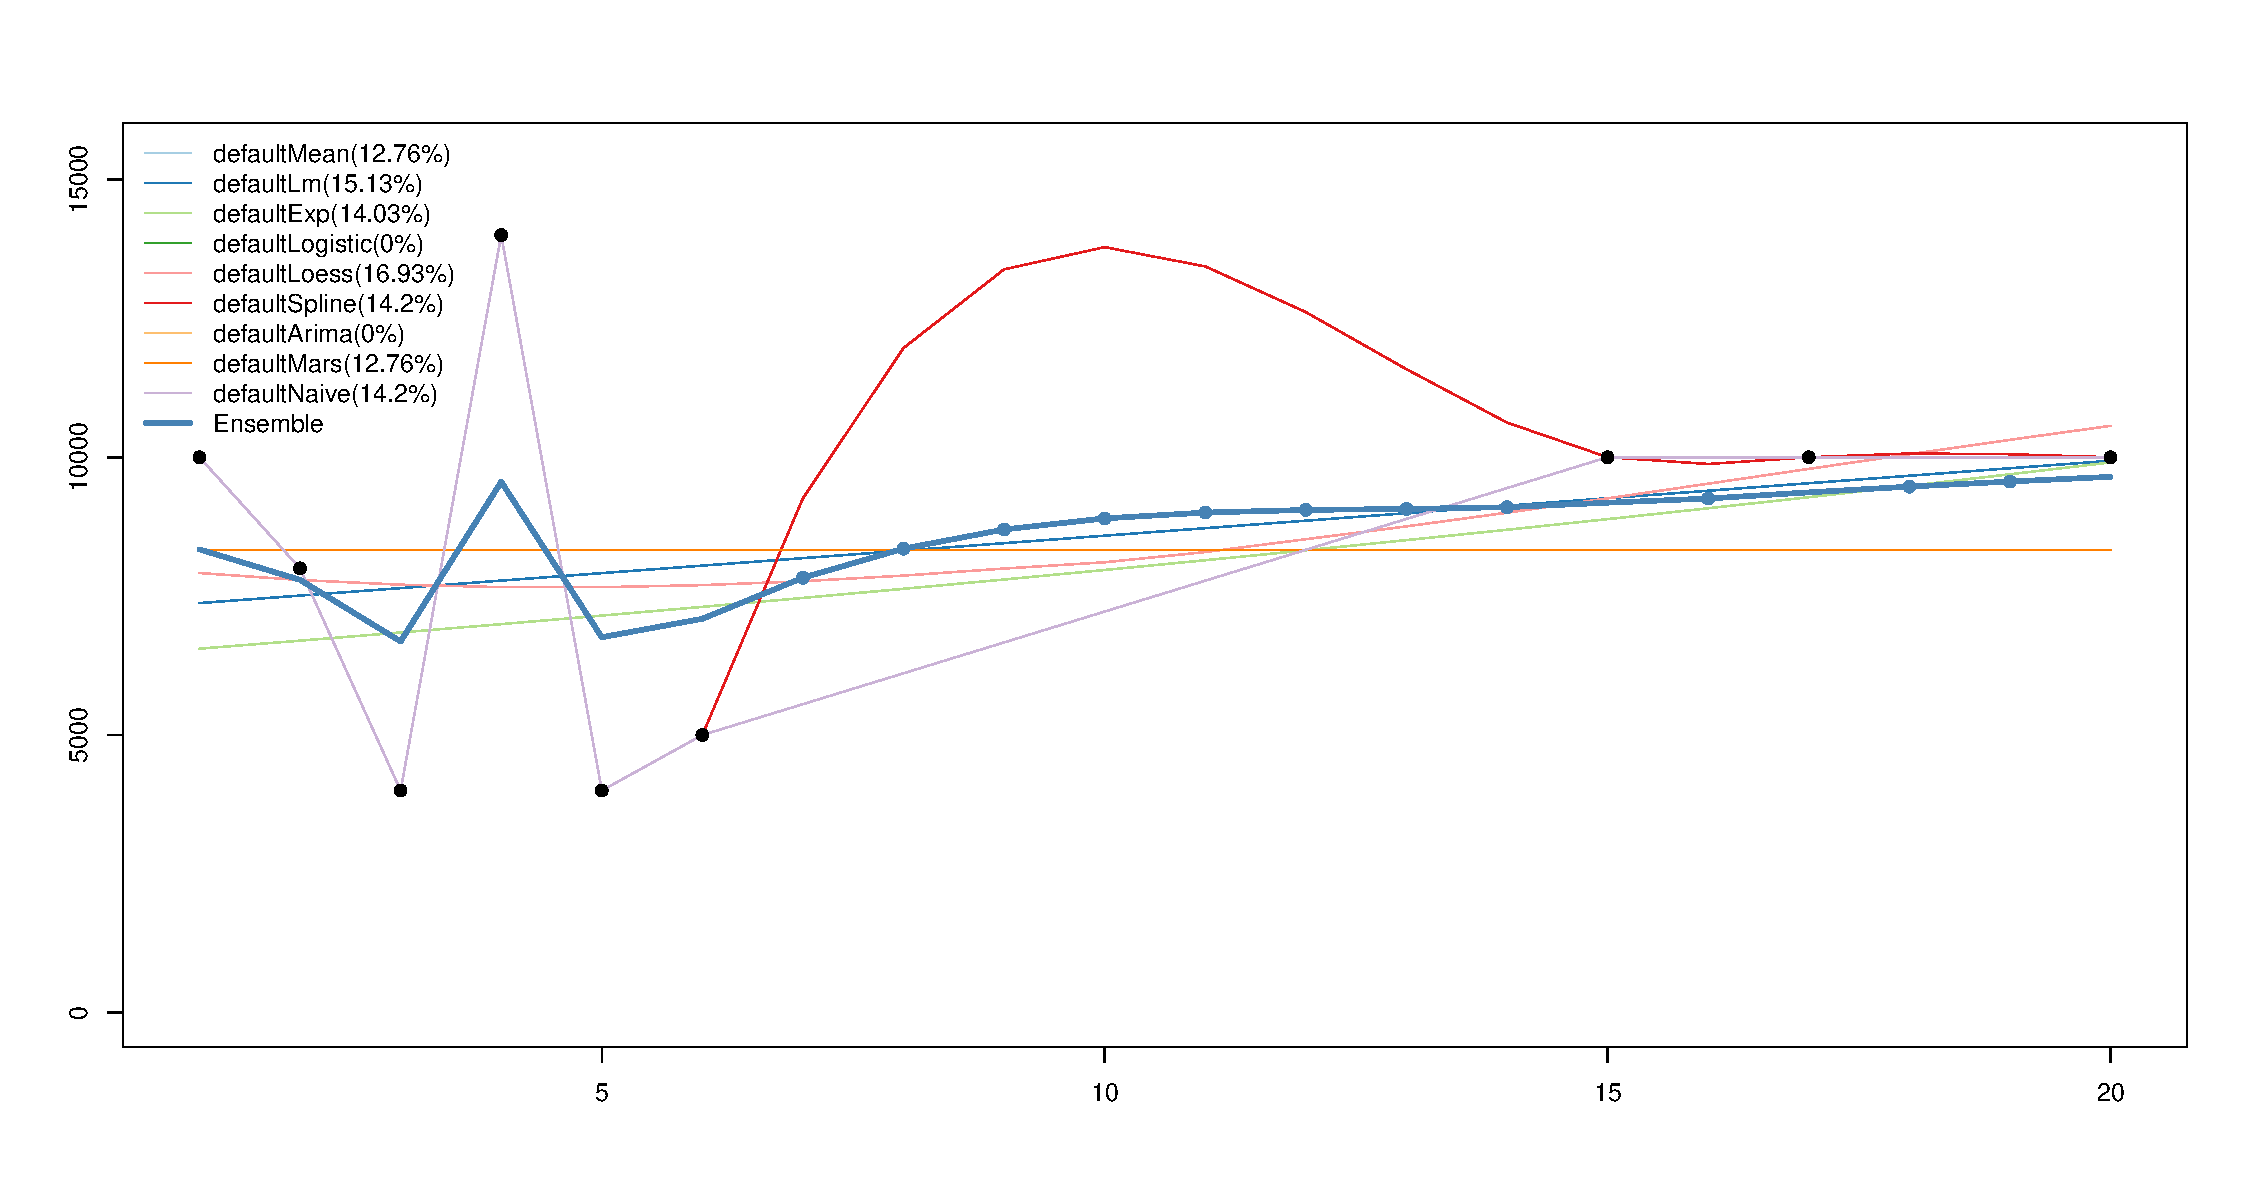
\includegraphics[width=\maxwidth]{figure/wheat-madagascar} 

}

\caption[In contrast to swaziland, the wheat production in Mauritania exhibits a simple shape]{In contrast to swaziland, the wheat production in Mauritania exhibits a simple shape. Almost equal weights were allocated to model which did not fail.\label{fig:wheat-madagascar}}
\end{figure}


\end{knitrout}


\begin{knitrout}
\definecolor{shadecolor}{rgb}{0.969, 0.969, 0.969}\color{fgcolor}\begin{figure}[!ht]


{\centering 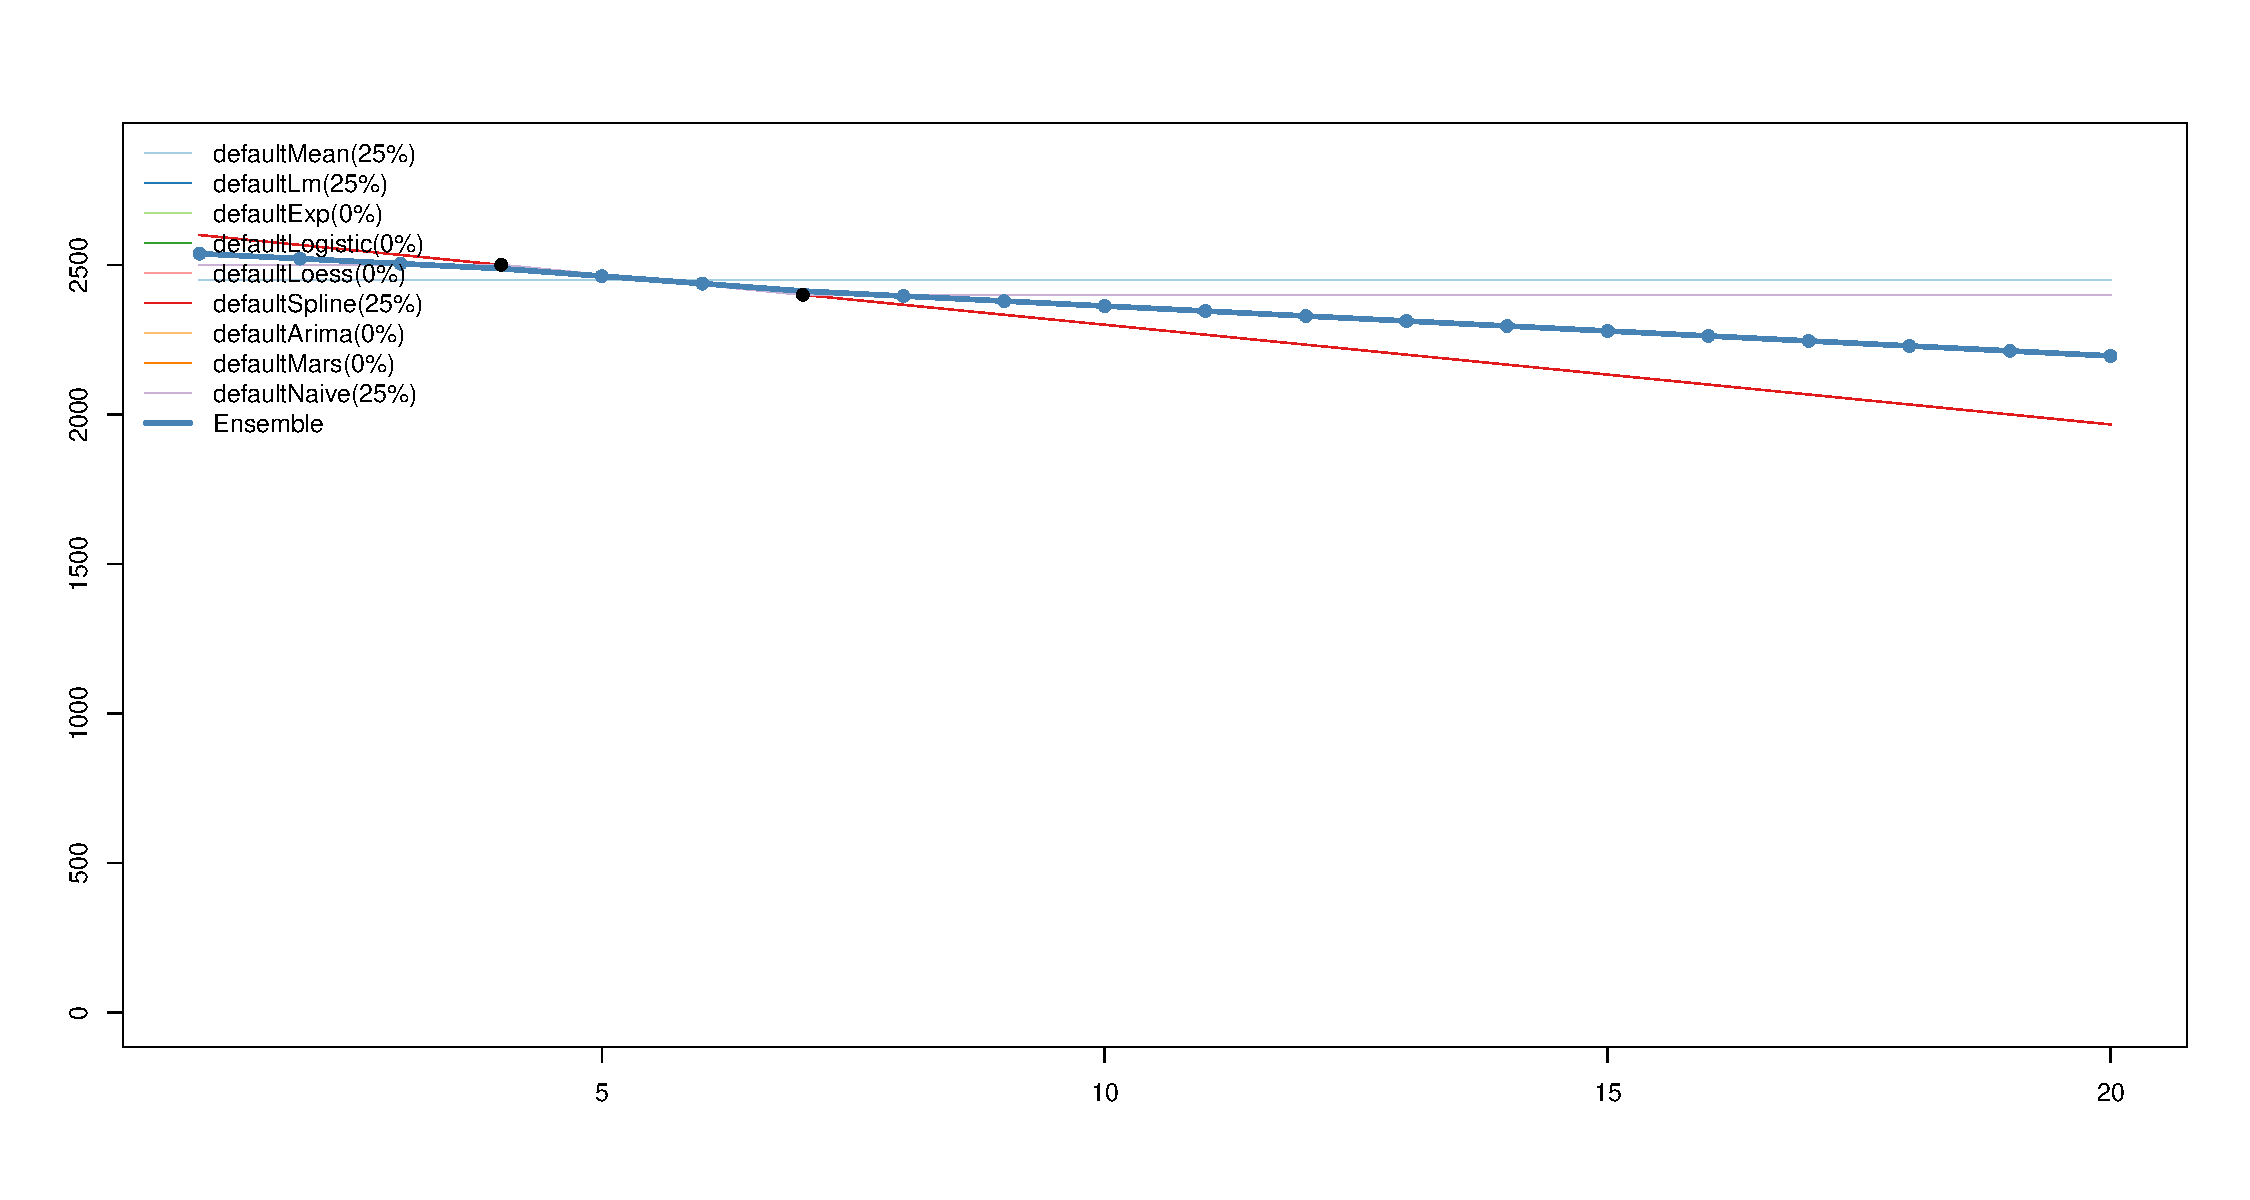
\includegraphics[width=\maxwidth]{figure/grape-zimbabwe} 

}

\caption[In this depiction, the grape of Zimbabwe is used for illustration]{In this depiction, the grape of Zimbabwe is used for illustration. In the case where there is not sufficient amount of data, the ensemble will collapse to form a simple model with strong agreements between the models.\label{fig:grape-zimbabwe}}
\end{figure}


\end{knitrout}

\begin{knitrout}
\definecolor{shadecolor}{rgb}{0.969, 0.969, 0.969}\color{fgcolor}\begin{figure}[!ht]


{\centering 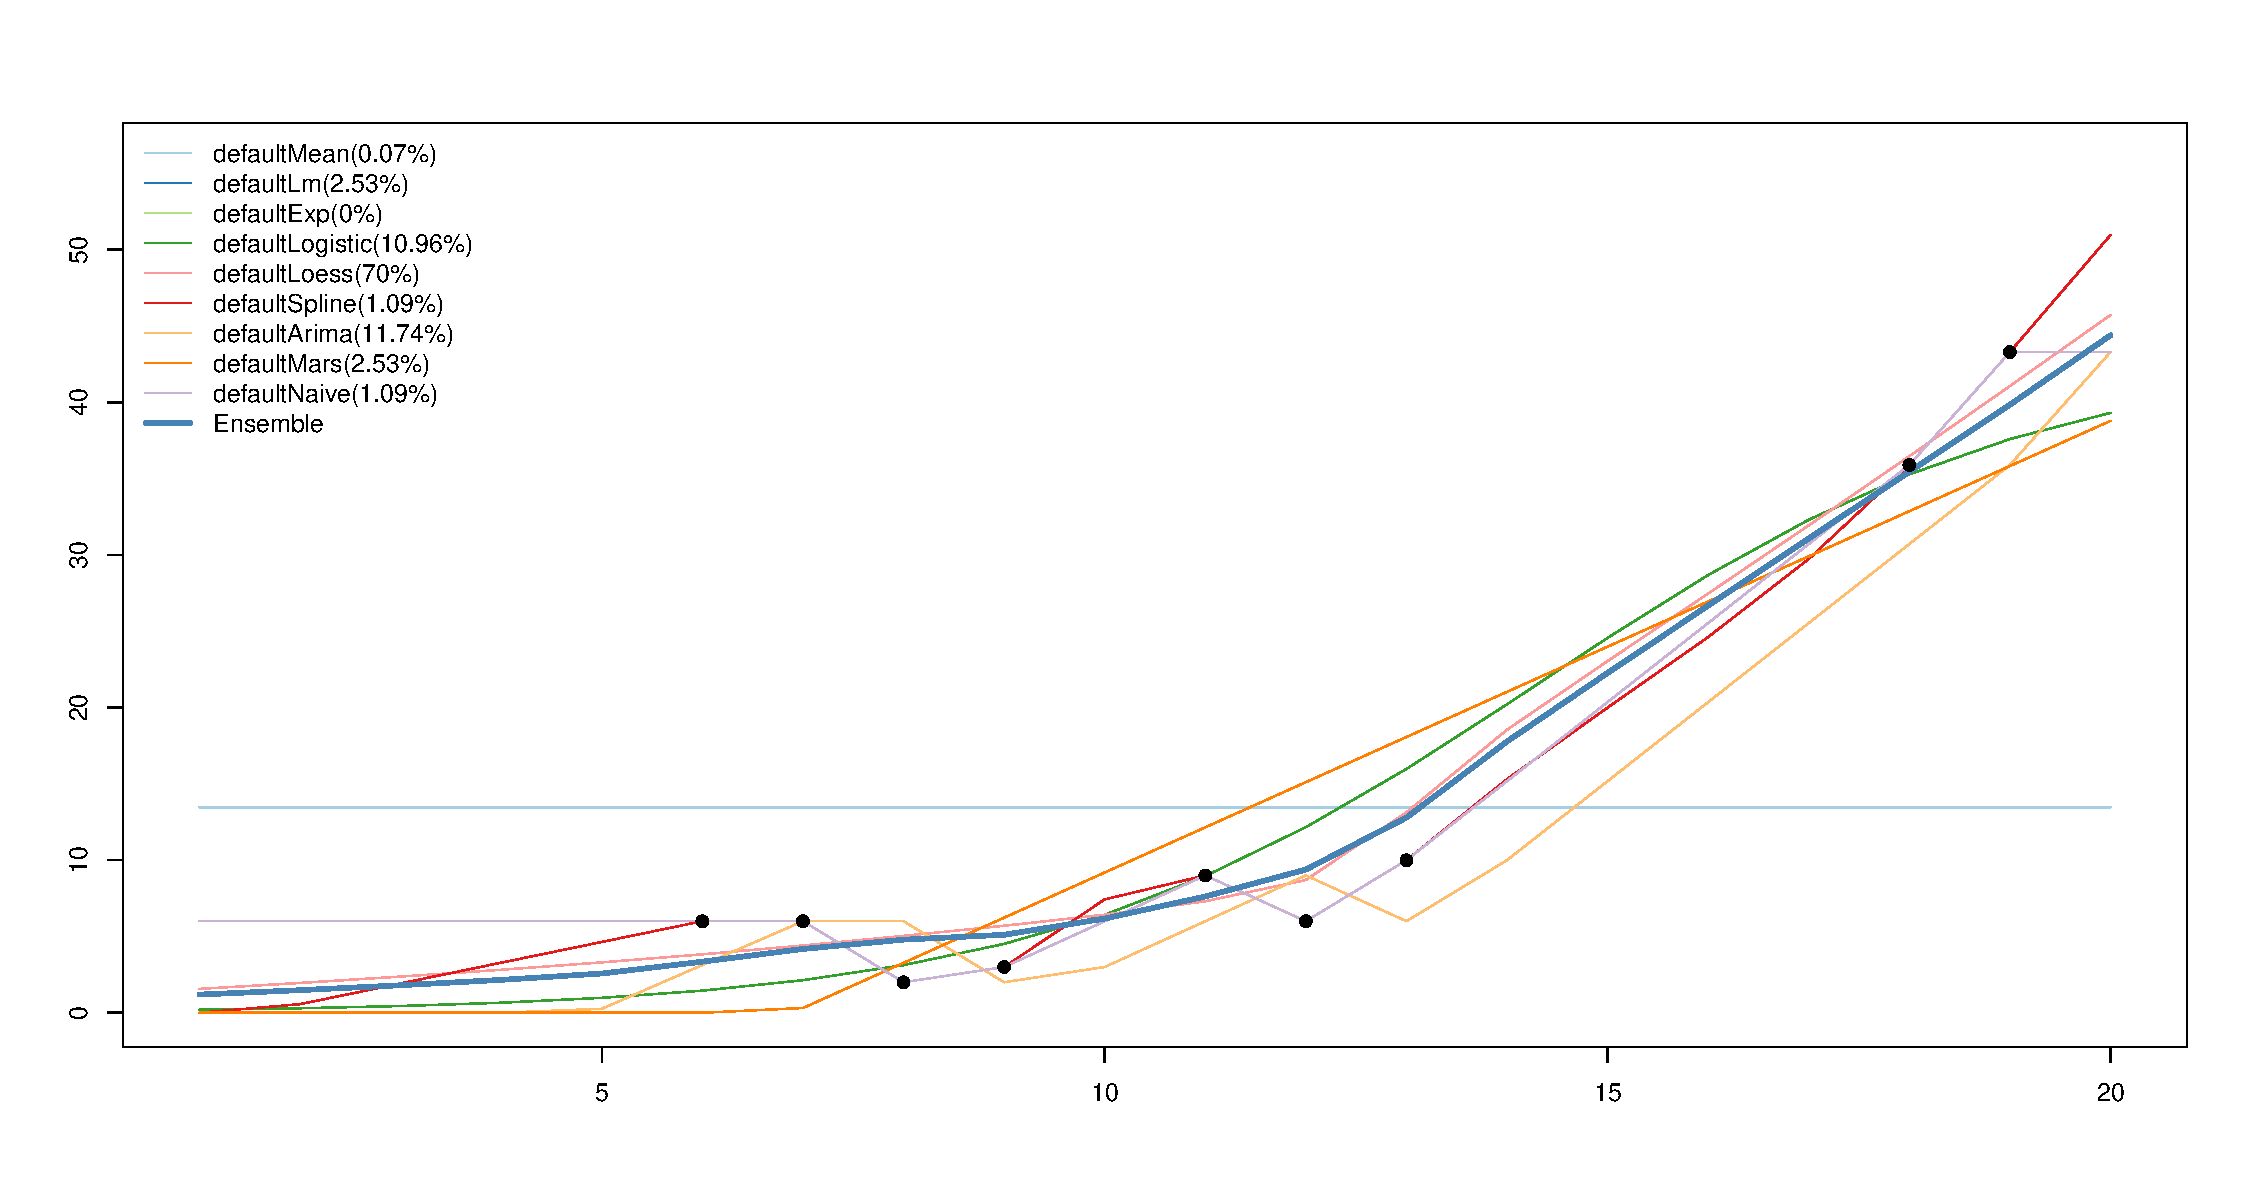
\includegraphics[width=\maxwidth]{figure/grape-kuwait} 

}

\caption[This time series for the grape productionn in Kuwait also displays simple exponential like growth]{This time series for the grape productionn in Kuwait also displays simple exponential like growth. Here, the smooth LOESS model obtained the highest weight and in fact reached the ceiling of 70 percent. The exponential failed because the default model requires that at least one point need to be observed at the first and the last 5 time point. This is to prevent the exponential model imputing values which are not supported by the data.\label{fig:grape-kuwait}}
\end{figure}


\end{knitrout}



\begin{knitrout}
\definecolor{shadecolor}{rgb}{0.969, 0.969, 0.969}\color{fgcolor}\begin{figure}[!ht]


{\centering 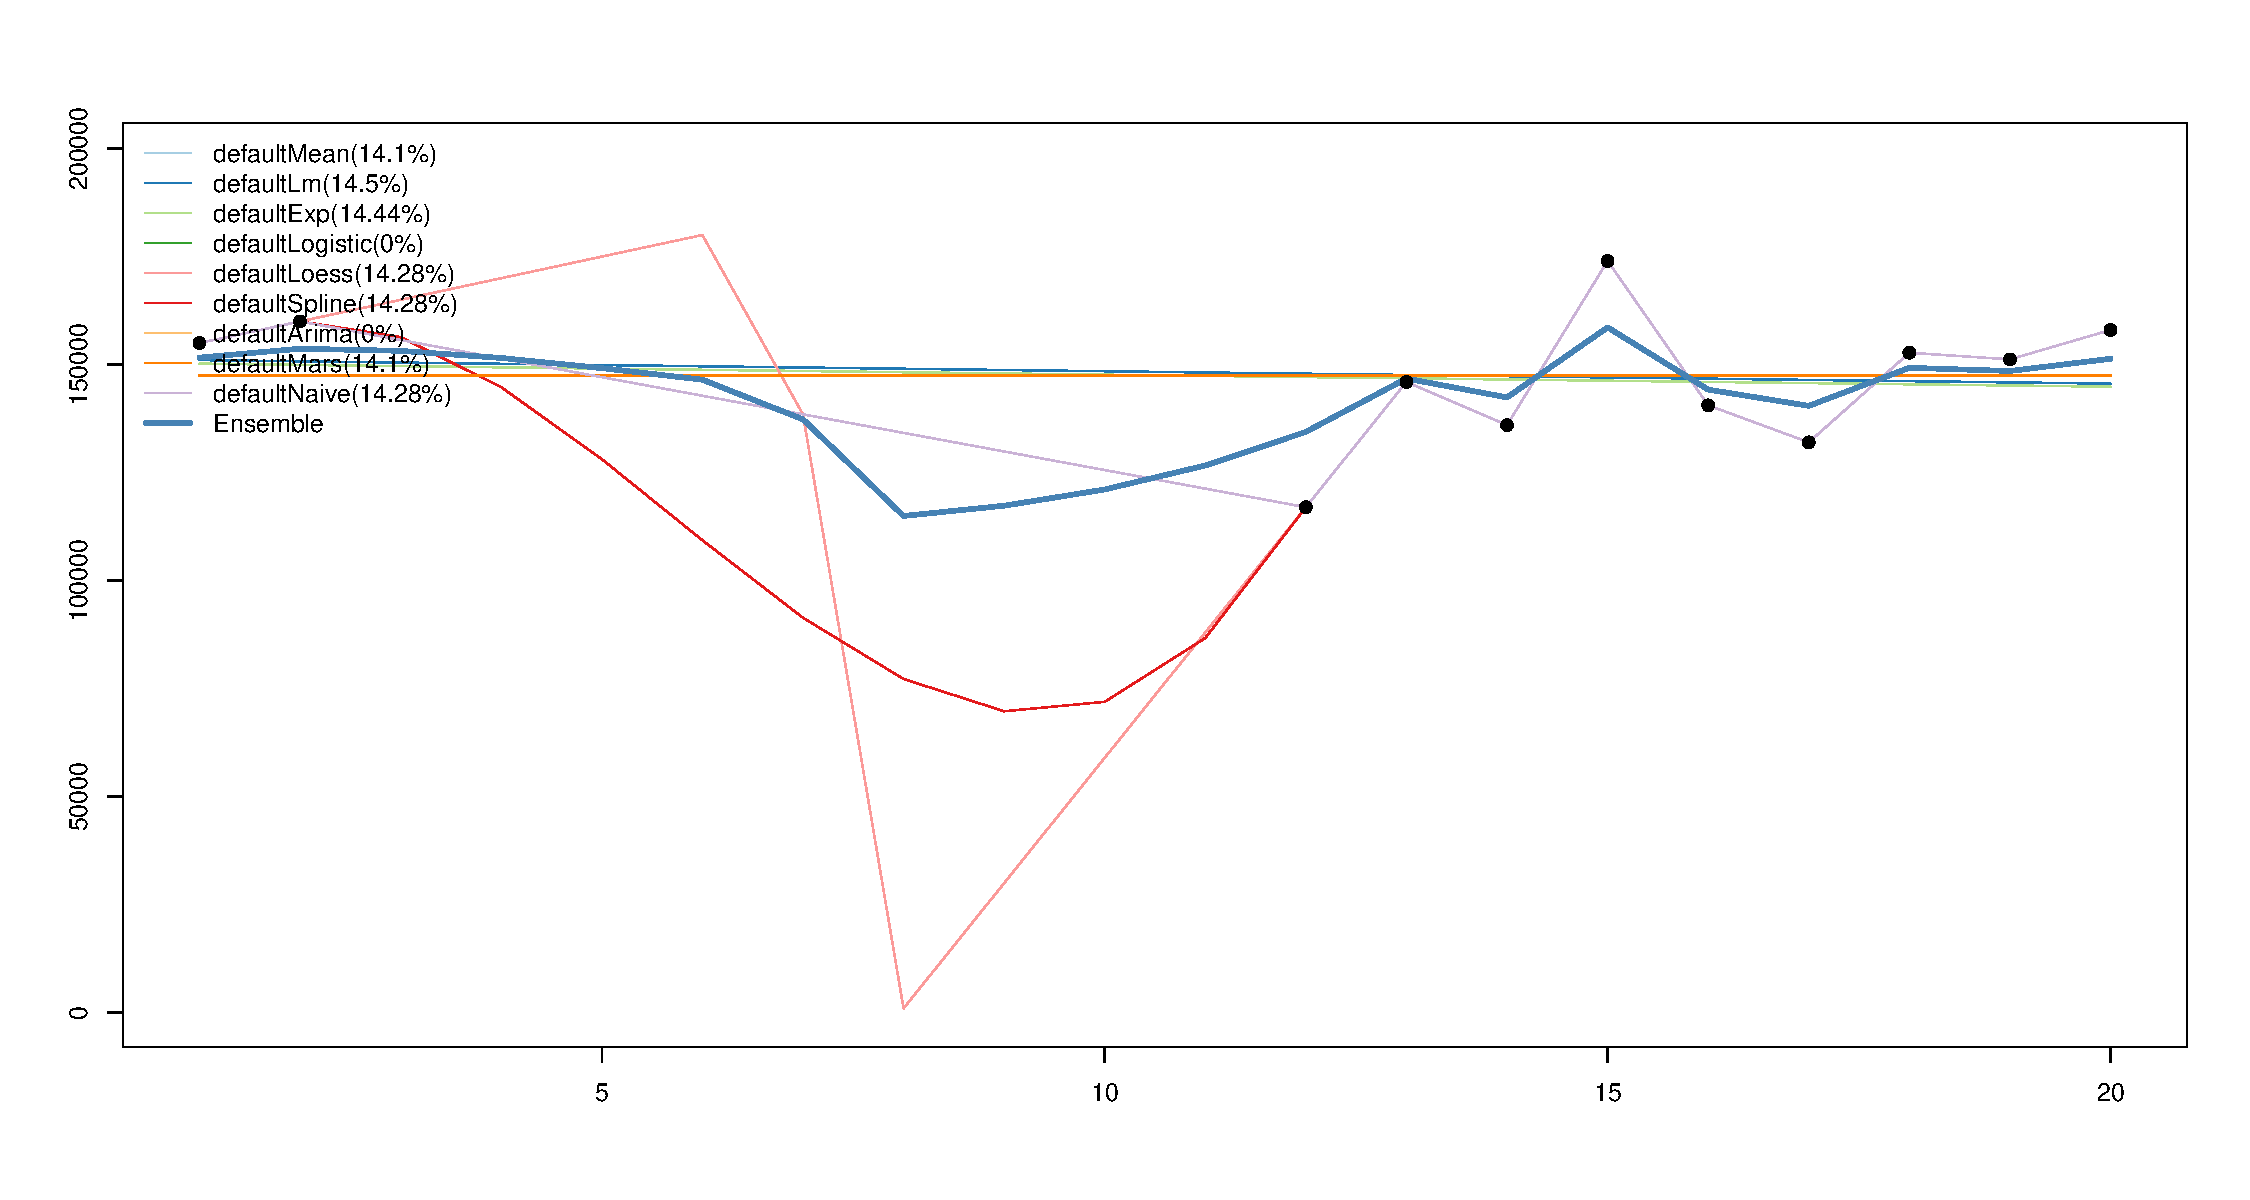
\includegraphics[width=\maxwidth]{figure/okra-ghana} 

}

\caption[There appears to be a gap in the series of the production of Okra for Iraq]{There appears to be a gap in the series of the production of Okra for Iraq. Most model collapse to a straight line close to the mean of the series, but both spline and loess captured the possible downward trend which is reflected in the dent in the final ensemble. \label{fig:okra-ghana}}
\end{figure}


\end{knitrout}


\begin{knitrout}
\definecolor{shadecolor}{rgb}{0.969, 0.969, 0.969}\color{fgcolor}\begin{figure}[!ht]


{\centering 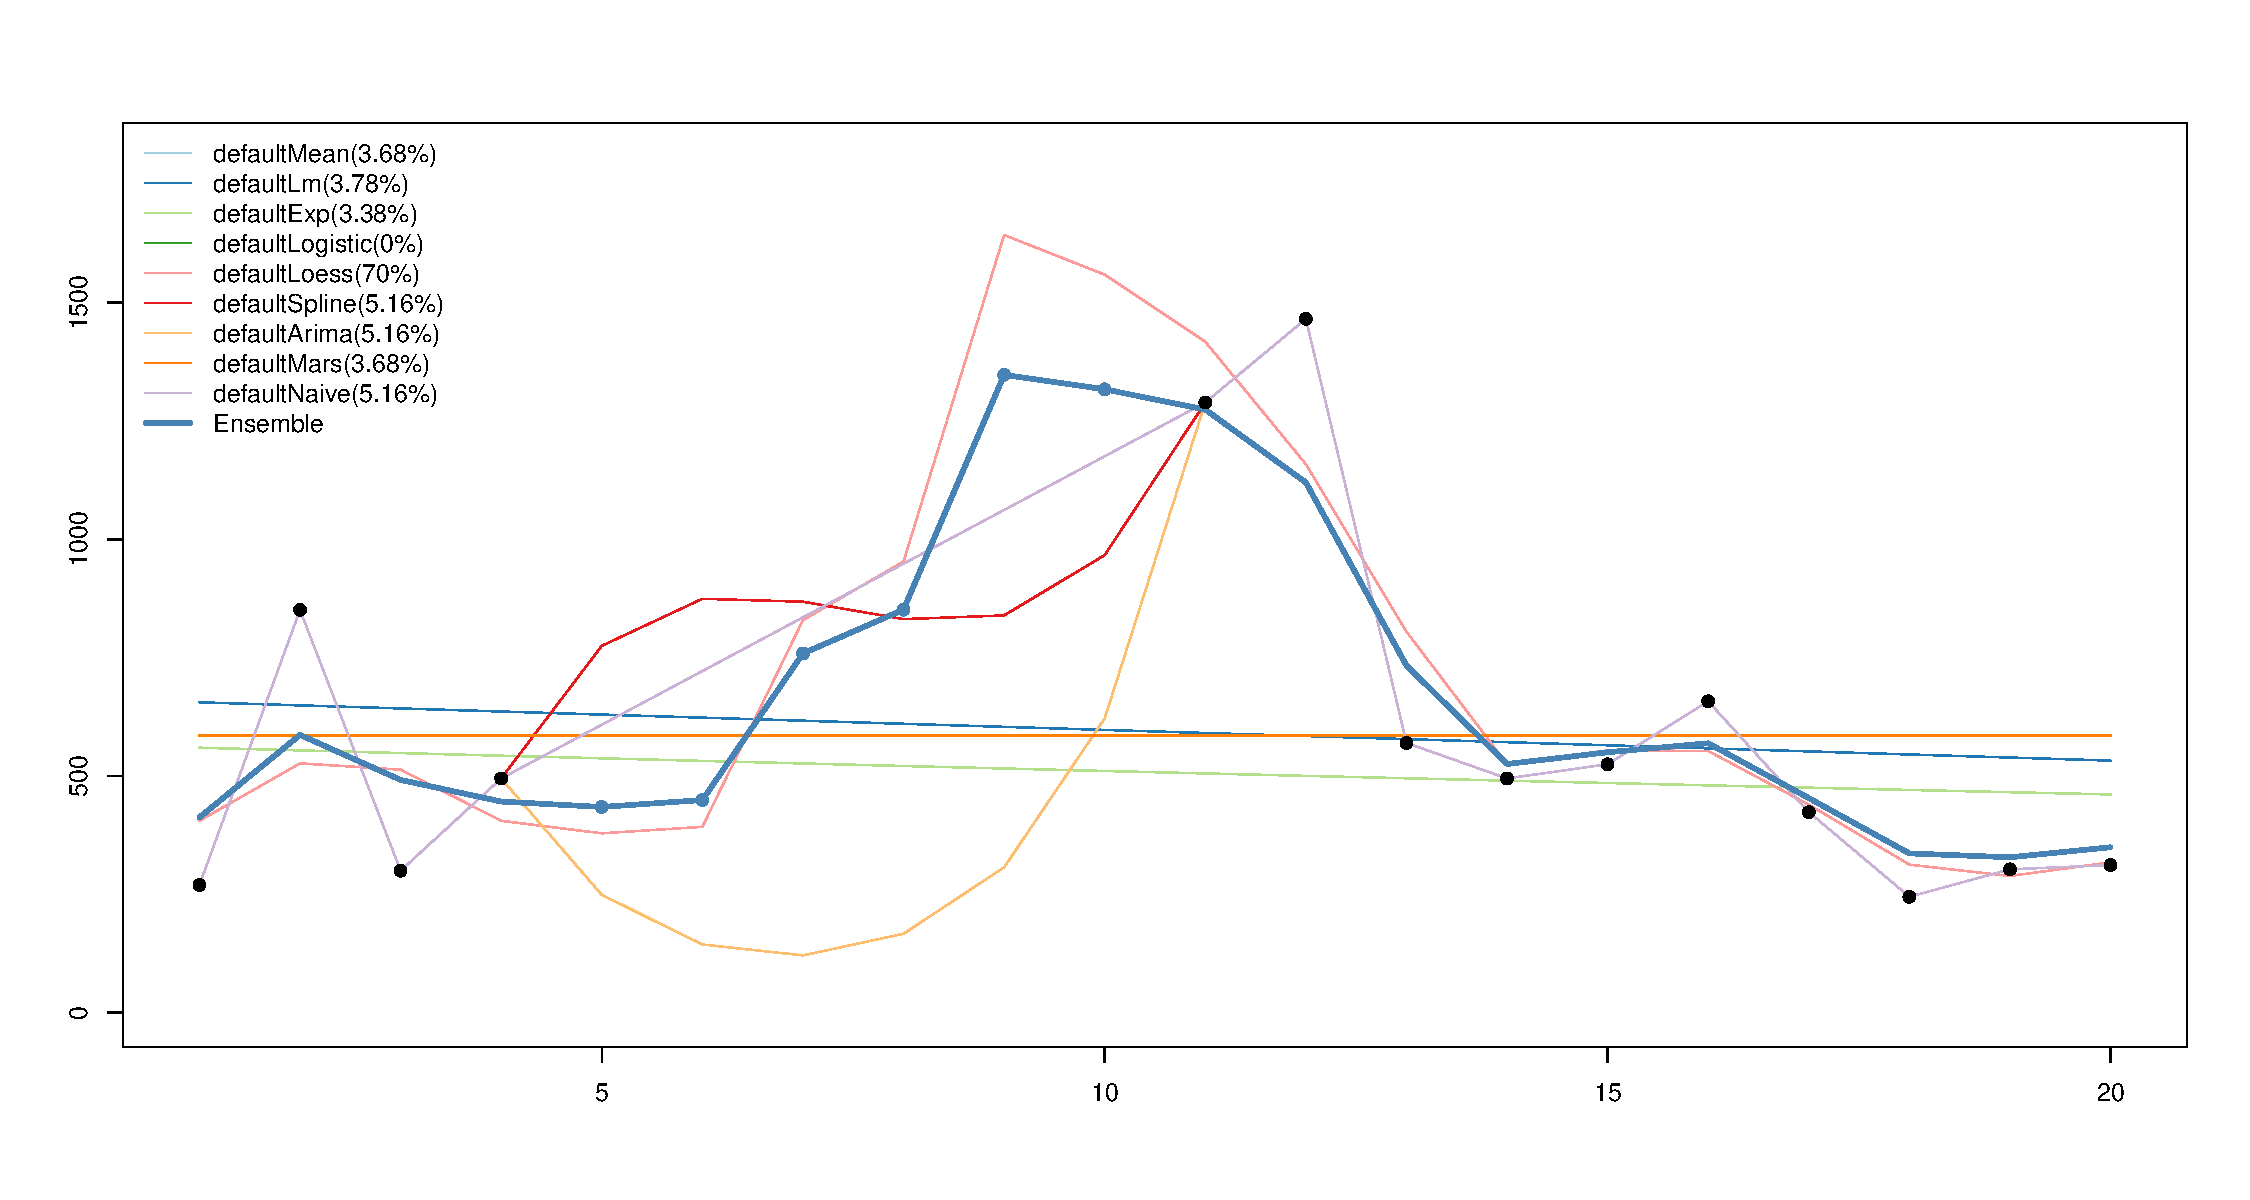
\includegraphics[width=\maxwidth]{figure/okra-barbados} 

}

\caption[Finally, a more complex example is shown here, the series is the production of Okra in Barbados]{Finally, a more complex example is shown here, the series is the production of Okra in Barbados. There were a few observation in the beginning of the series, then in the center of the time series the production doubled before falling to prior level. A relative complex model is required to fit such a time series, loess took most of the weight with the remaining weight assigned equally to other model.\label{fig:okra-barbados}}
\end{figure}


\end{knitrout}

\FloatBarrier

The examples demonstrates that the model is flexible, able to capture
from the simplest linear trend to more complex behaviours without the
need for model selection. Further, with carefully selected and fine
tuned component models, the ensemble will exhibit extremely robust
characteristics.


\FloatBarrier
\subsection{Imputation for Area Harvested}

After the imputation of production and yield, area harvested is left
to balance to satisfiy the identity equation.\\


\subsection{Use of external variables}
The proposed methodology does not employ any other variables for
several reasons. First, the external variables may also contain
missing value and often they may actually in fact be more sparse than
the dataset we are trying to impute. Secondly, the selection of
variables may be difficult. Difference in commodity nature, market
structure, commercialization and other conditions calls for different
information set for prediction. Finally, even if a set of data can be
selected, the use of external variables will require large resources
to maintain and specific design set up to be used under various
imputation setting.\\


\section{Case Studies}

The imputation of the three commodities are presented in this
section. Due to the limitation that this is a dynamic generated paper
we have only include the cross-country information for the imputation
of the yield.


\subsection{Wheat}

\begin{knitrout}
\definecolor{shadecolor}{rgb}{0.969, 0.969, 0.969}\color{fgcolor}\begin{figure}[!ht]


{\centering 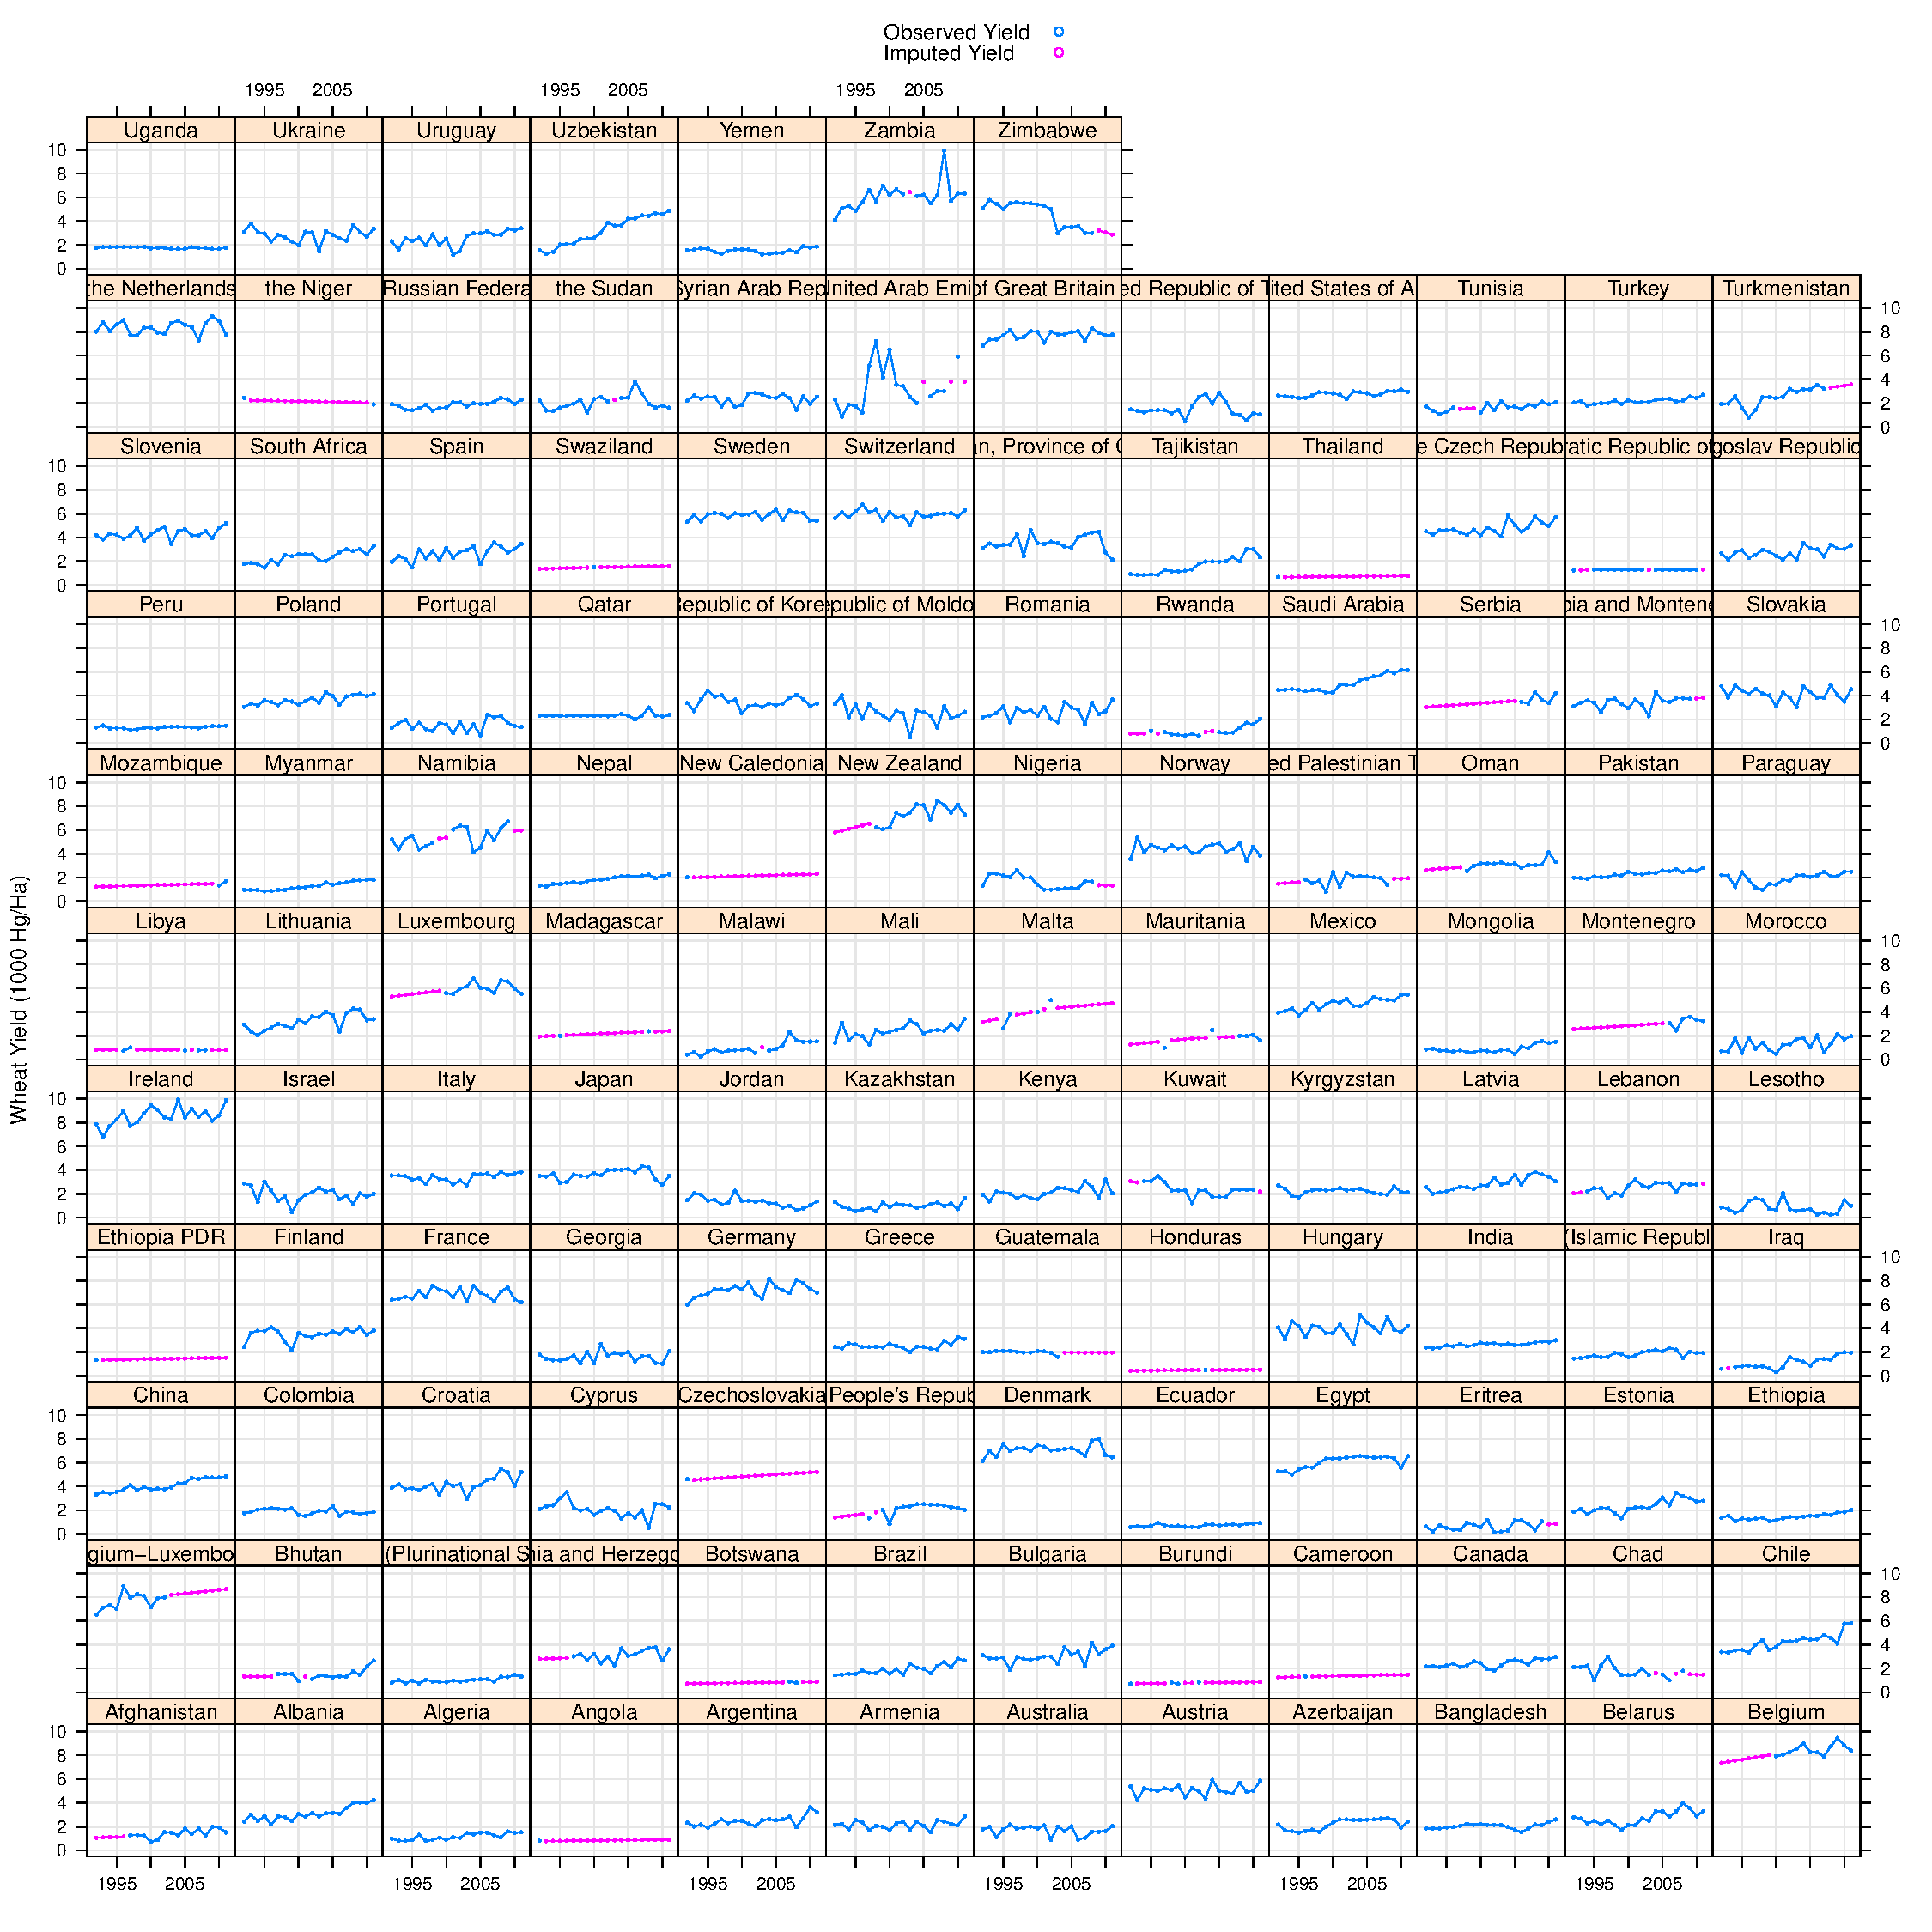
\includegraphics[width=\maxwidth]{figure/wheat-yield-imputed} 

}

\caption[We can see the imputation of yield in purple seems to produce reasonable values]{We can see the imputation of yield in purple seems to produce reasonable values.\label{fig:wheat-yield-imputed}}
\end{figure}


\end{knitrout}

\begin{knitrout}
\definecolor{shadecolor}{rgb}{0.969, 0.969, 0.969}\color{fgcolor}\begin{figure}[!ht]


{\centering 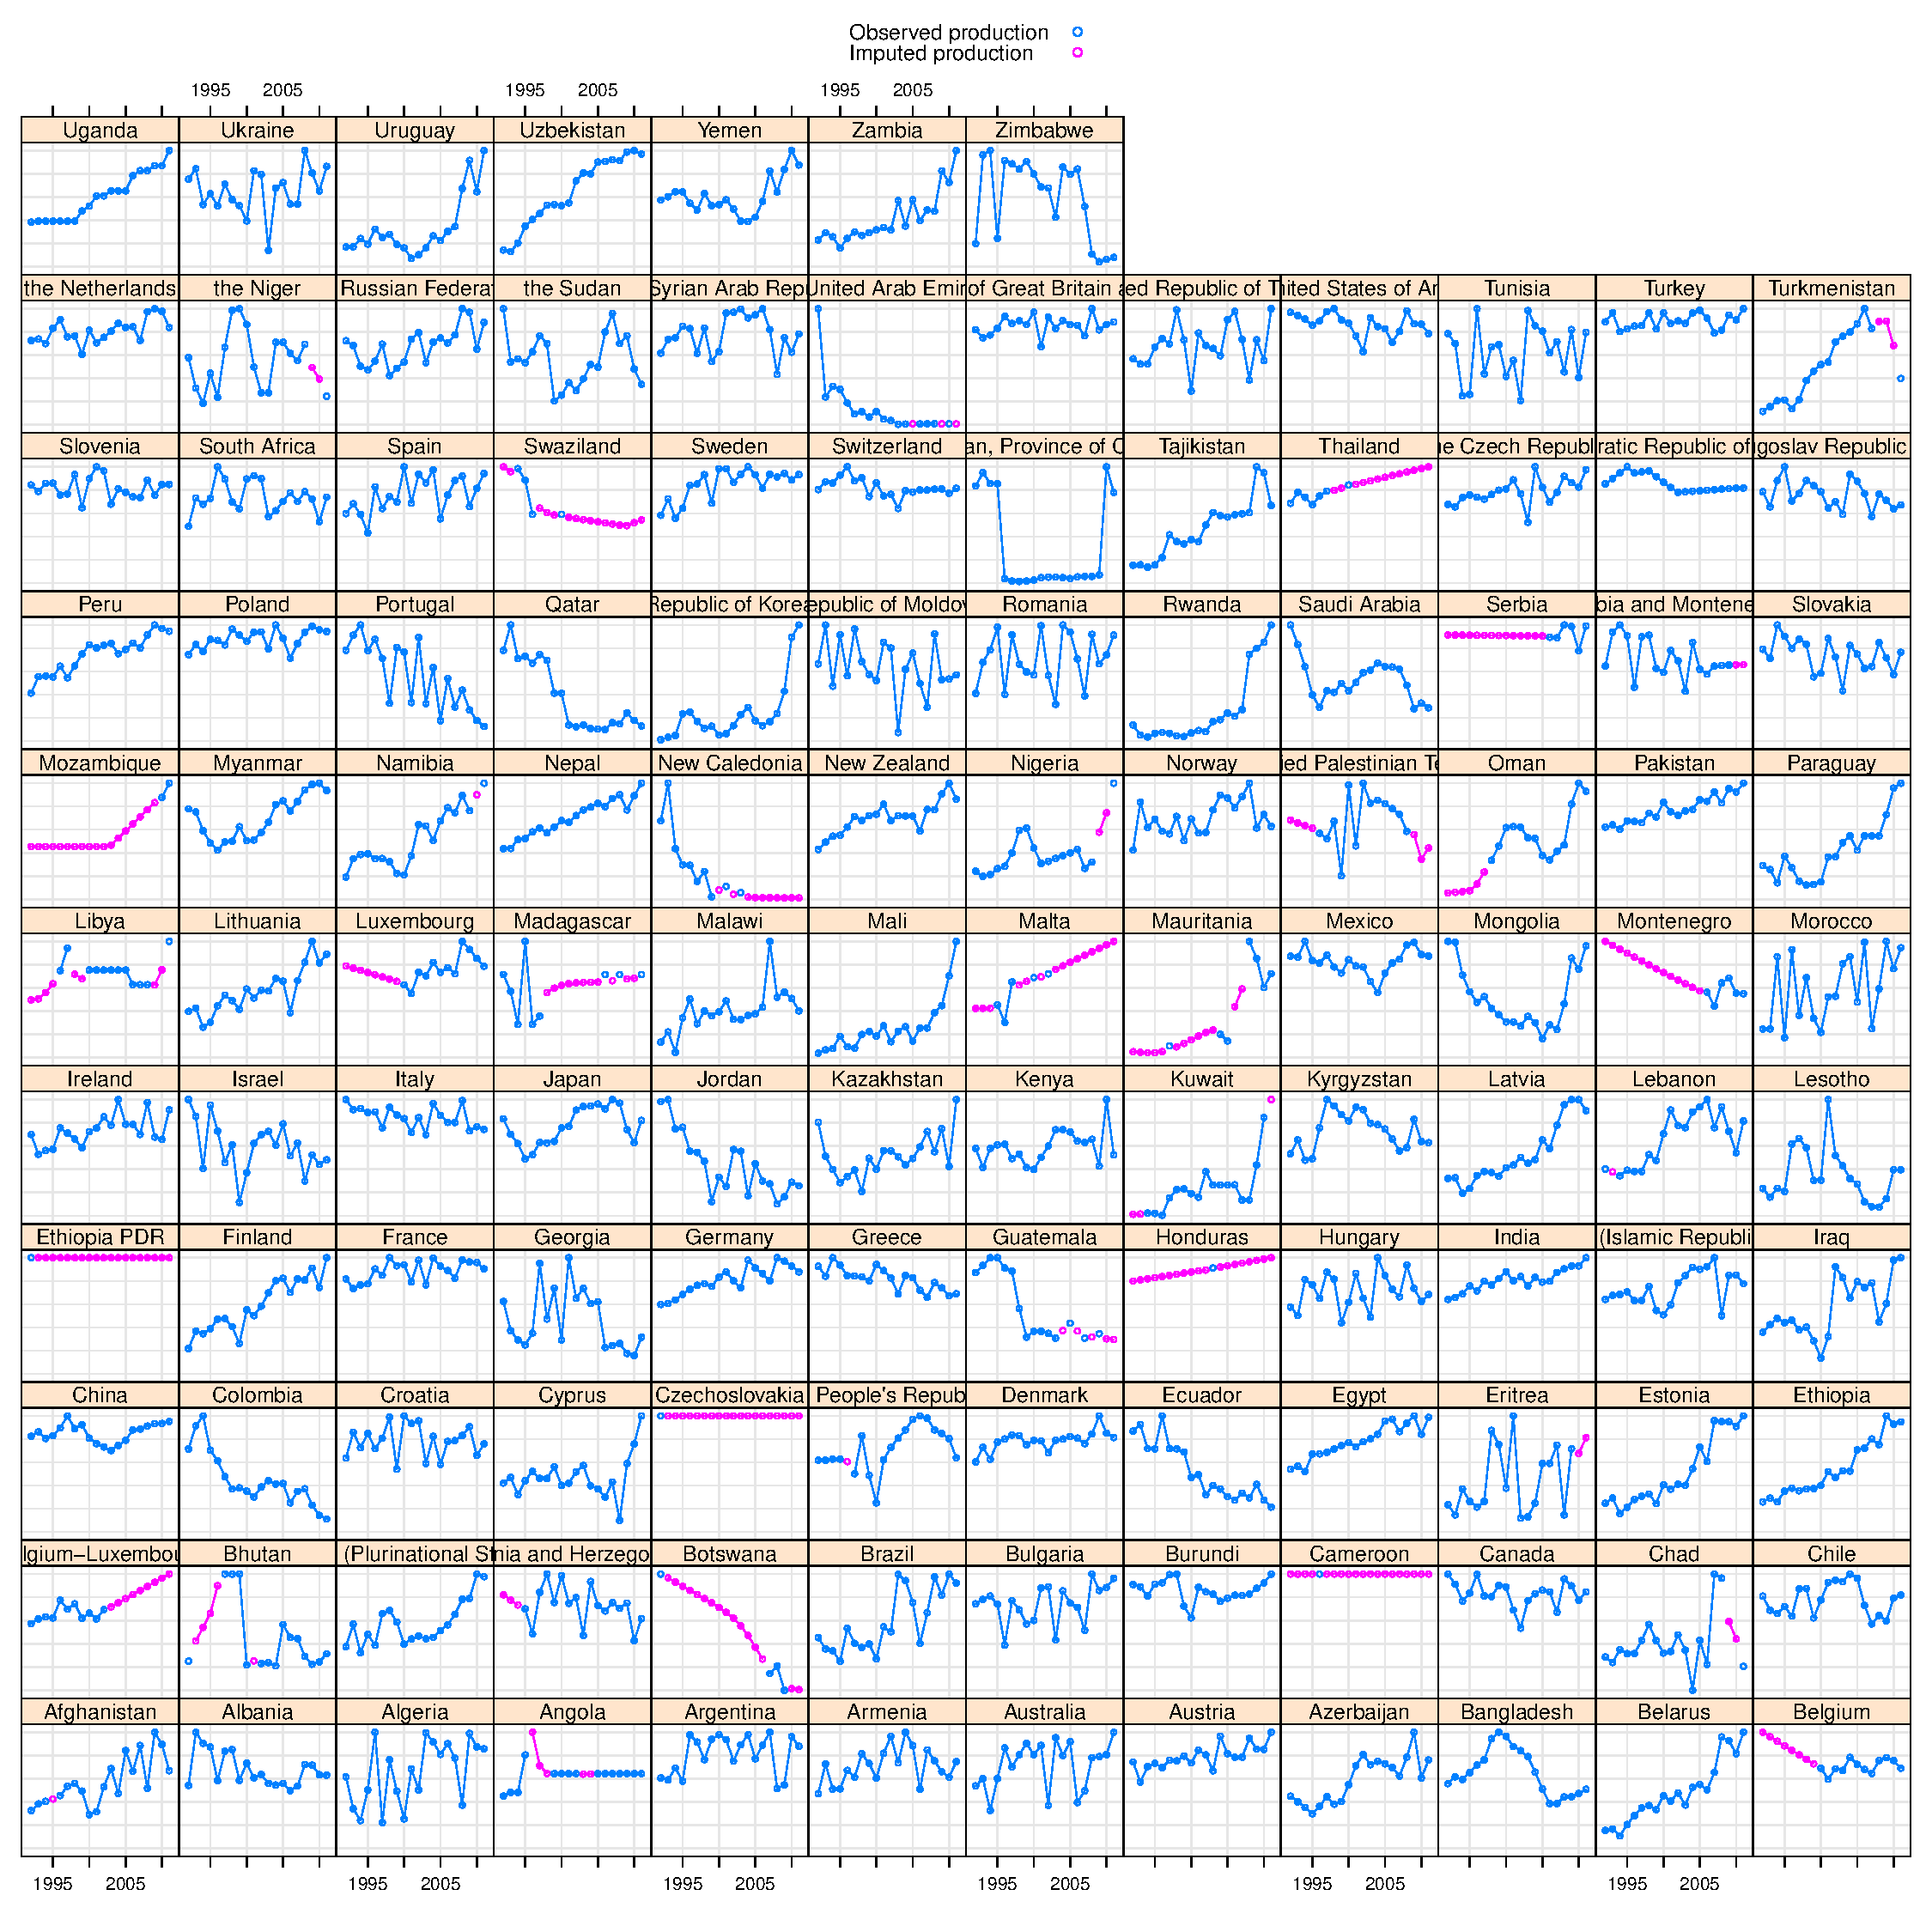
\includegraphics[width=\maxwidth]{figure/wheat-production-imputed} 

}

\caption[There does not appear to be any peculariy in any of the imputation of the production of wheat]{There does not appear to be any peculariy in any of the imputation of the production of wheat.\label{fig:wheat-production-imputed}}
\end{figure}


\end{knitrout}

\begin{knitrout}
\definecolor{shadecolor}{rgb}{0.969, 0.969, 0.969}\color{fgcolor}\begin{figure}[!ht]


{\centering 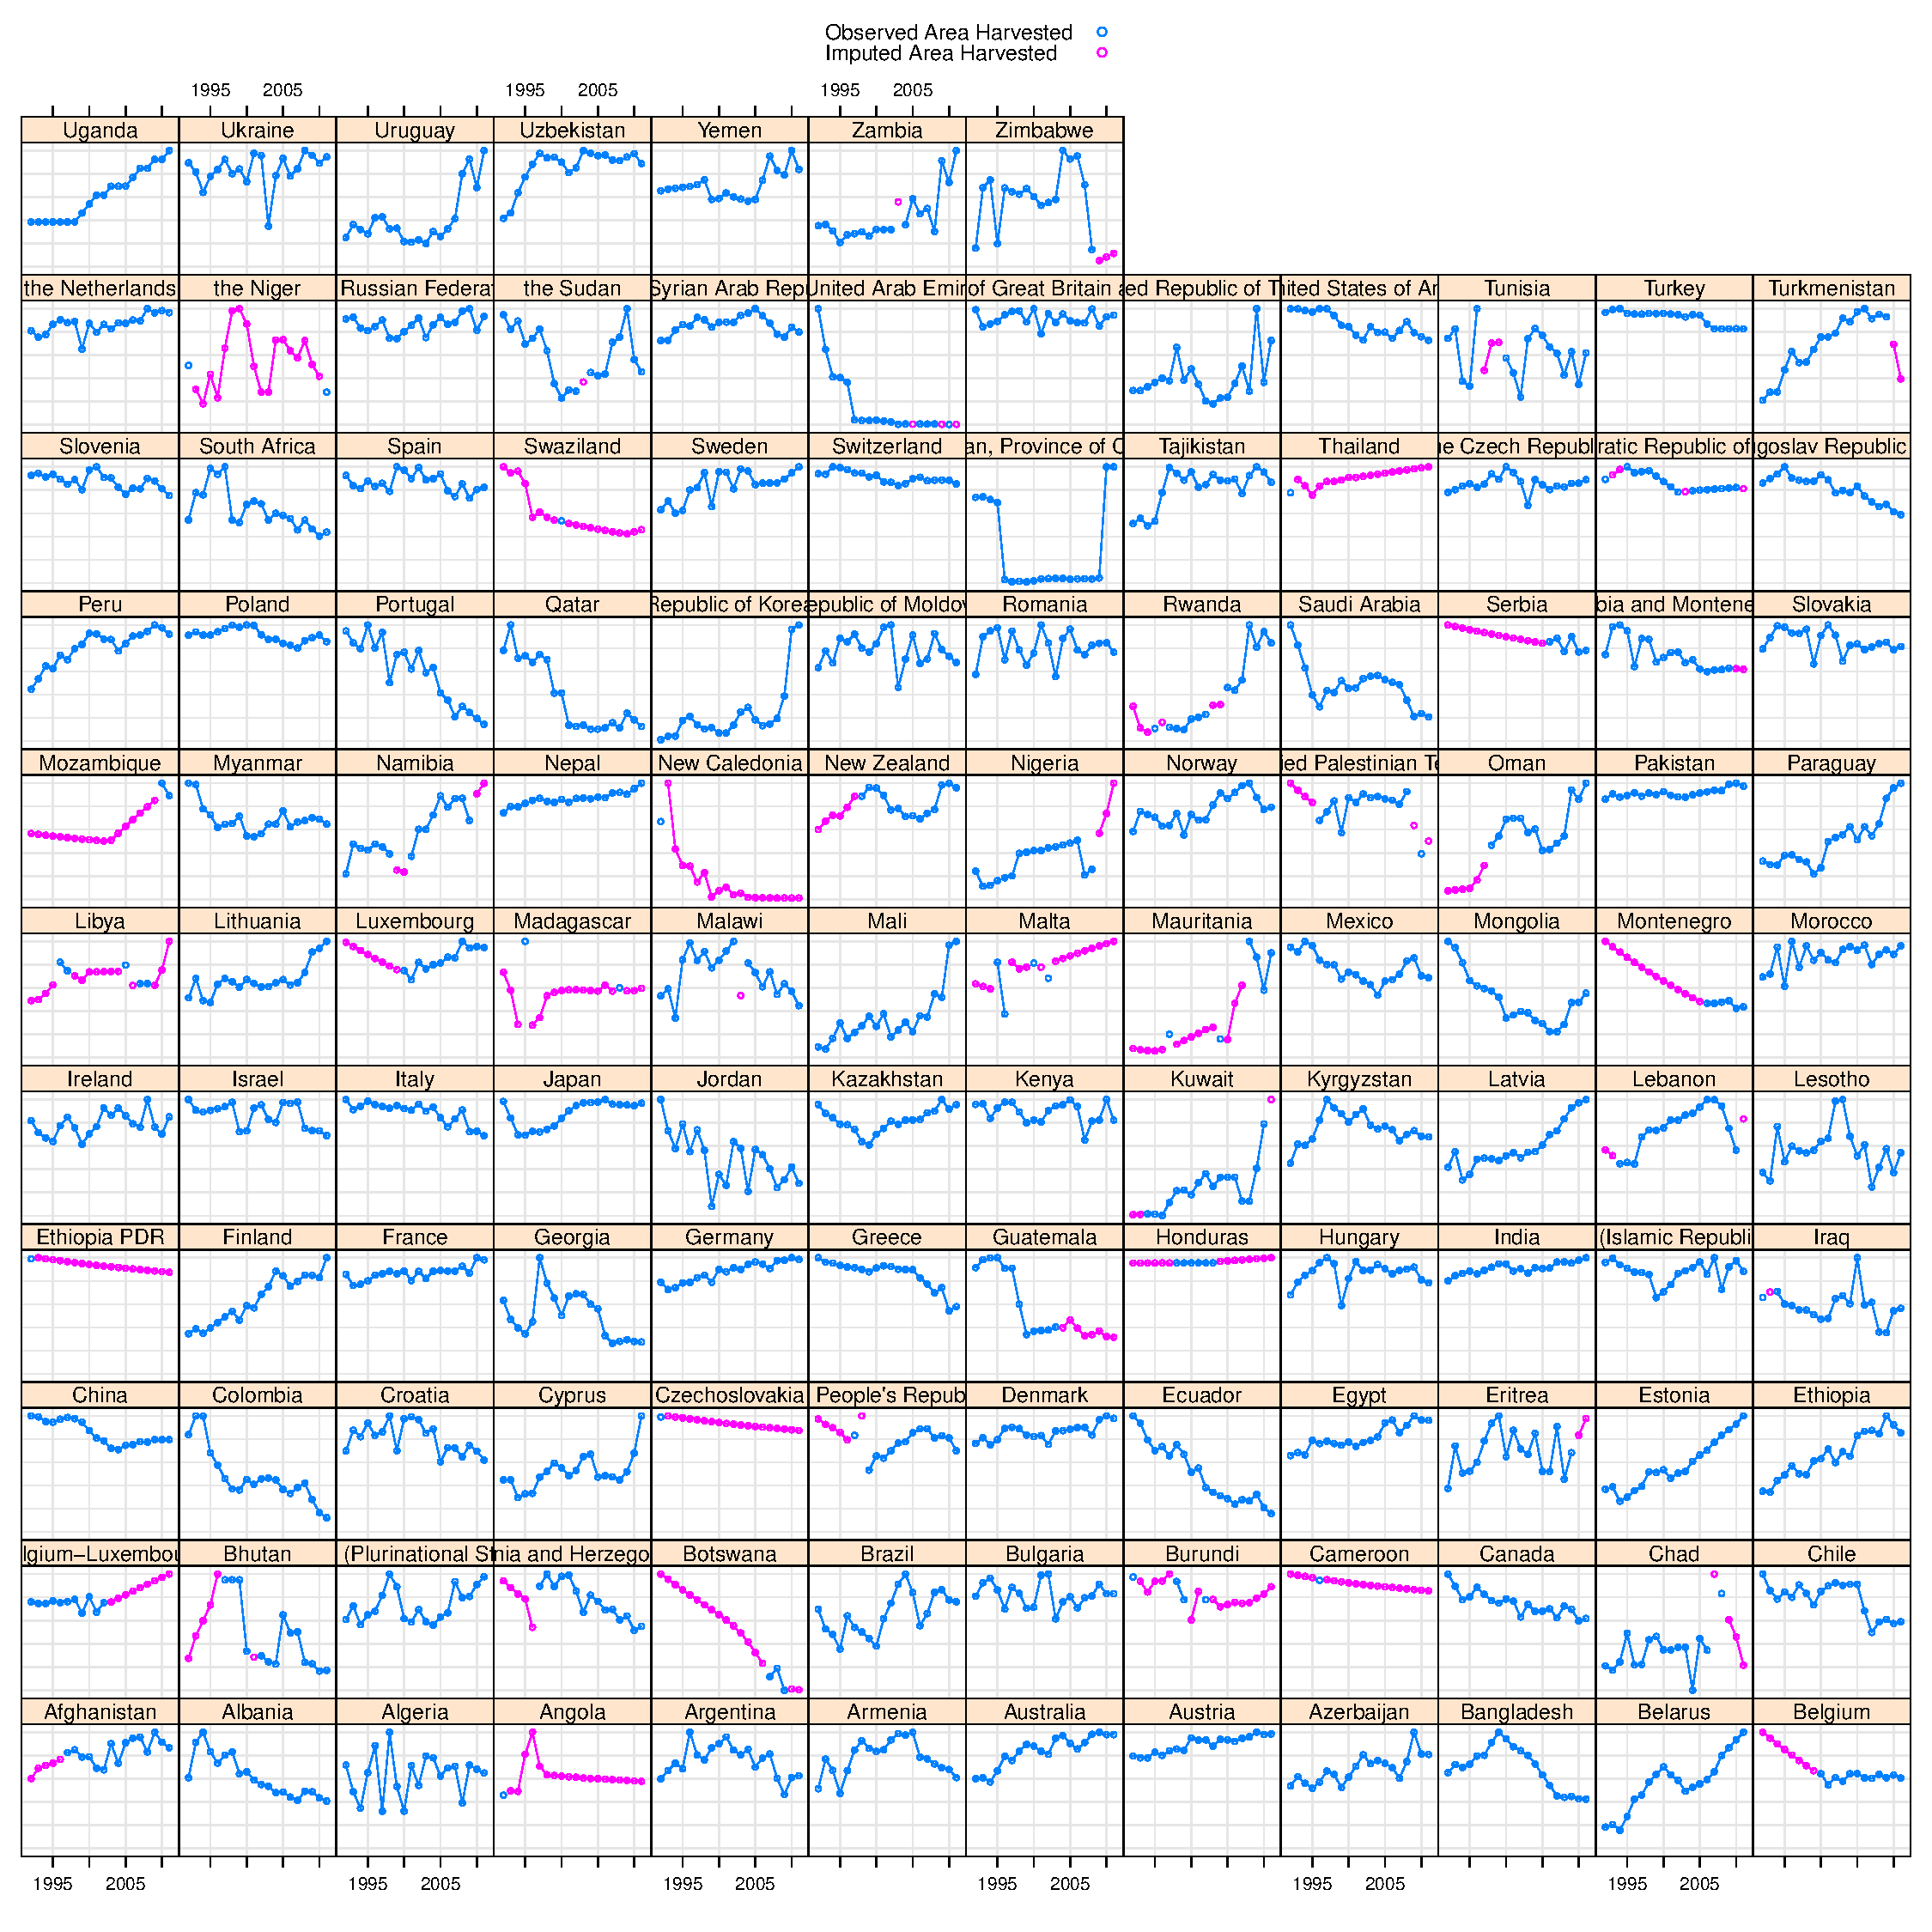
\includegraphics[width=\maxwidth]{figure/wheat-areaharvested-imputed} 

}

\caption[The balance of area harvested also does not show any sign of divergence or problematic symptoms]{The balance of area harvested also does not show any sign of divergence or problematic symptoms.\label{fig:wheat-areaharvested-imputed}}
\end{figure}


\end{knitrout}

\FloatBarrier
\subsection{Grape}

\begin{knitrout}
\definecolor{shadecolor}{rgb}{0.969, 0.969, 0.969}\color{fgcolor}\begin{figure}[!ht]


{\centering 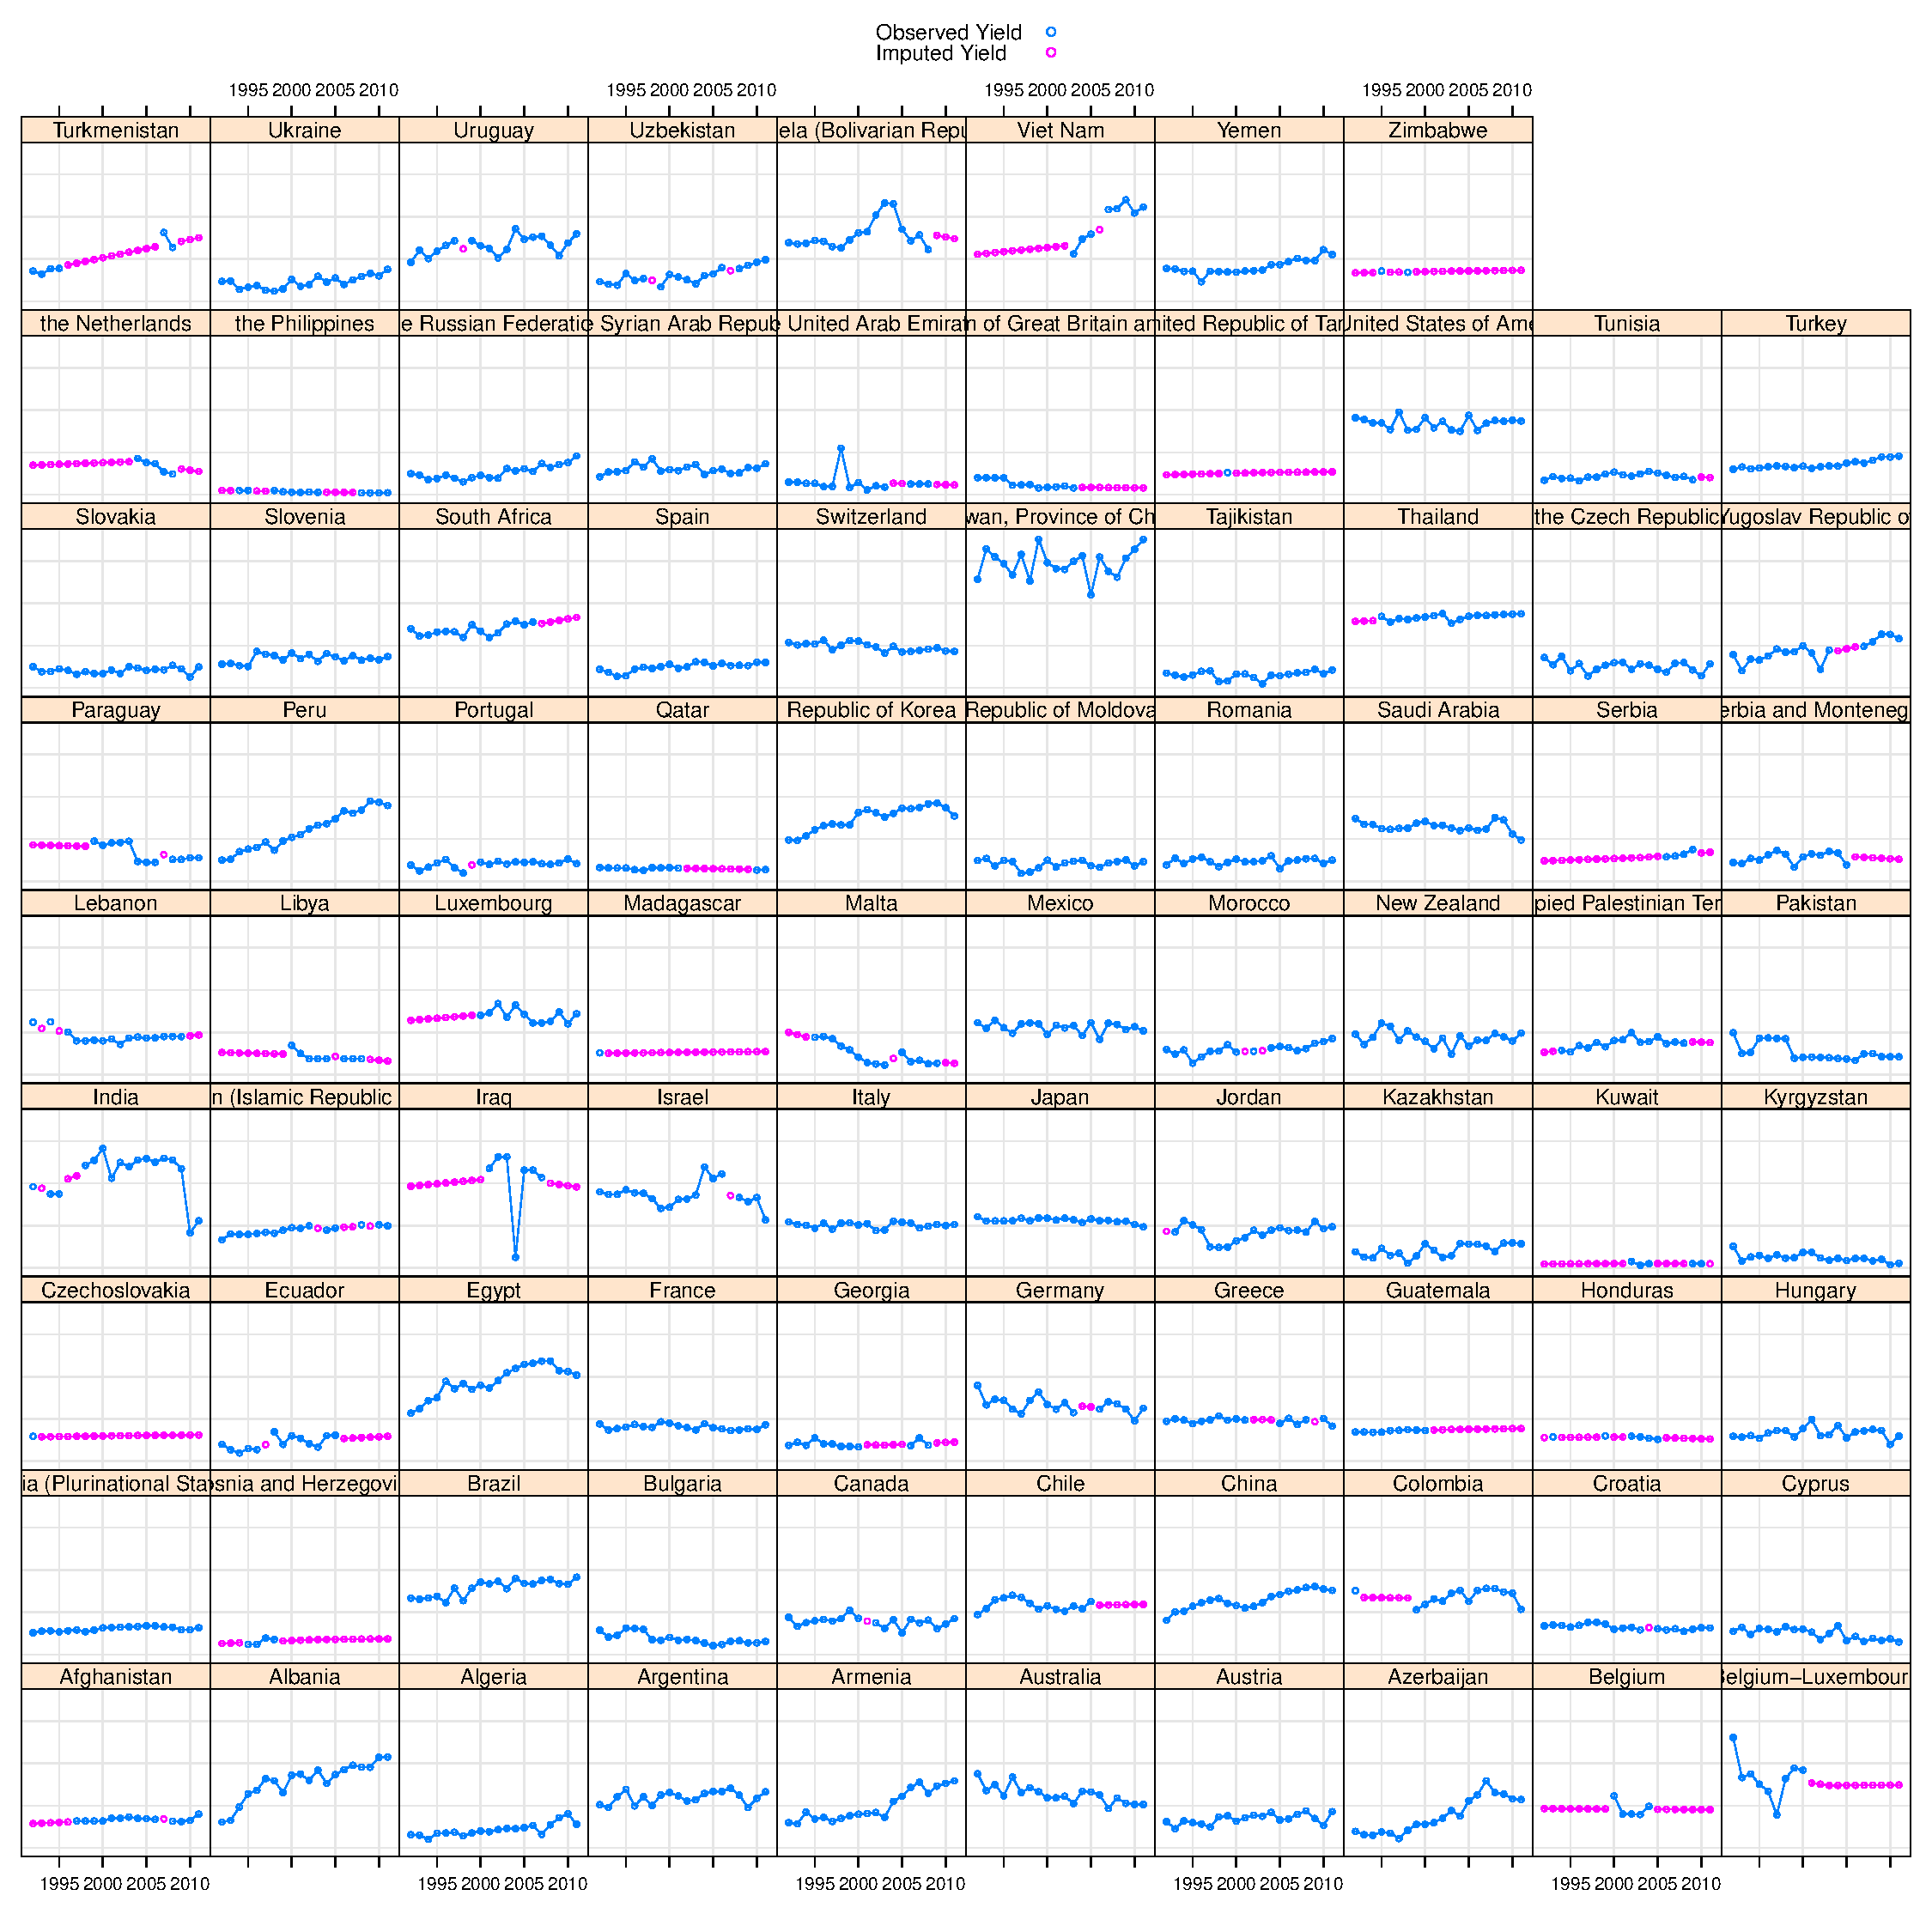
\includegraphics[width=\maxwidth]{figure/grape-yield-imputed} 

}

\caption[The imputation of yield also appears to be reasonable, even in the case for Iraq the linear mixed model is not severely influenced by the one off event]{The imputation of yield also appears to be reasonable, even in the case for Iraq the linear mixed model is not severely influenced by the one off event.\label{fig:grape-yield-imputed}}
\end{figure}


\end{knitrout}


\begin{knitrout}
\definecolor{shadecolor}{rgb}{0.969, 0.969, 0.969}\color{fgcolor}\begin{figure}[!ht]


{\centering 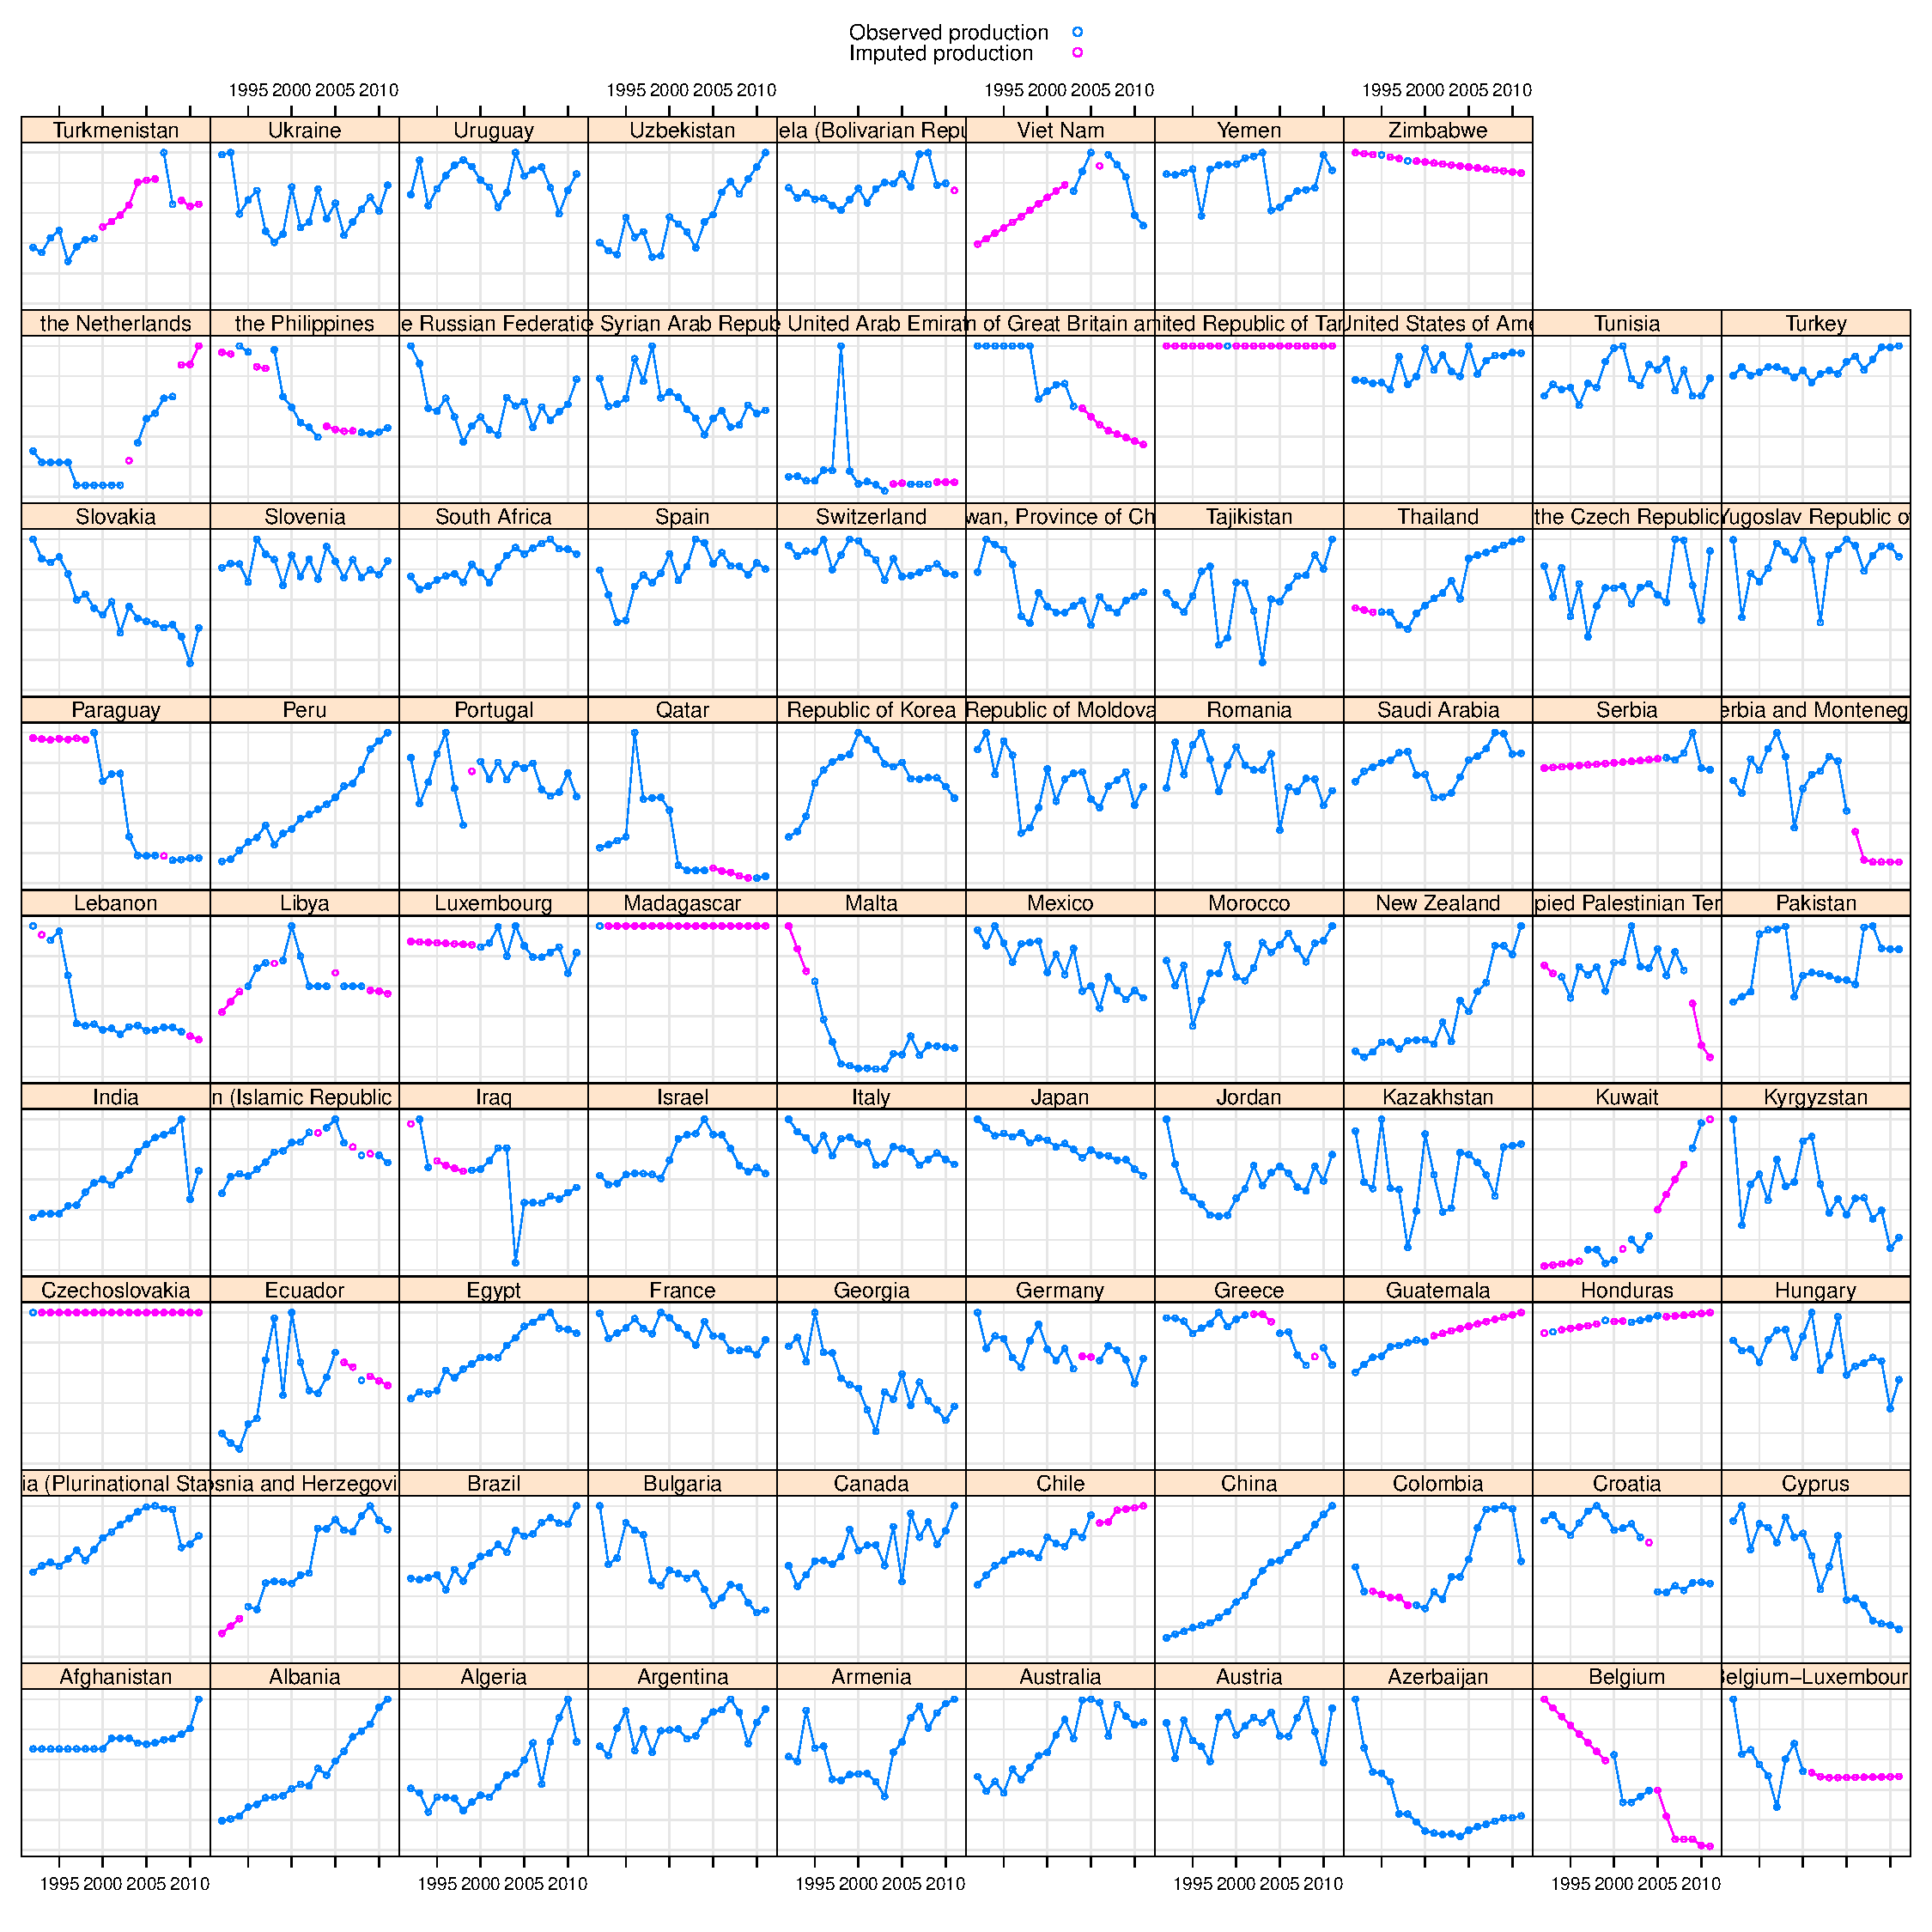
\includegraphics[width=\maxwidth]{figure/grape-production-imputed} 

}

\caption[The imputation of grape prodution]{The imputation of grape prodution.\label{fig:grape-production-imputed}}
\end{figure}


\end{knitrout}

\begin{knitrout}
\definecolor{shadecolor}{rgb}{0.969, 0.969, 0.969}\color{fgcolor}\begin{figure}[!ht]


{\centering 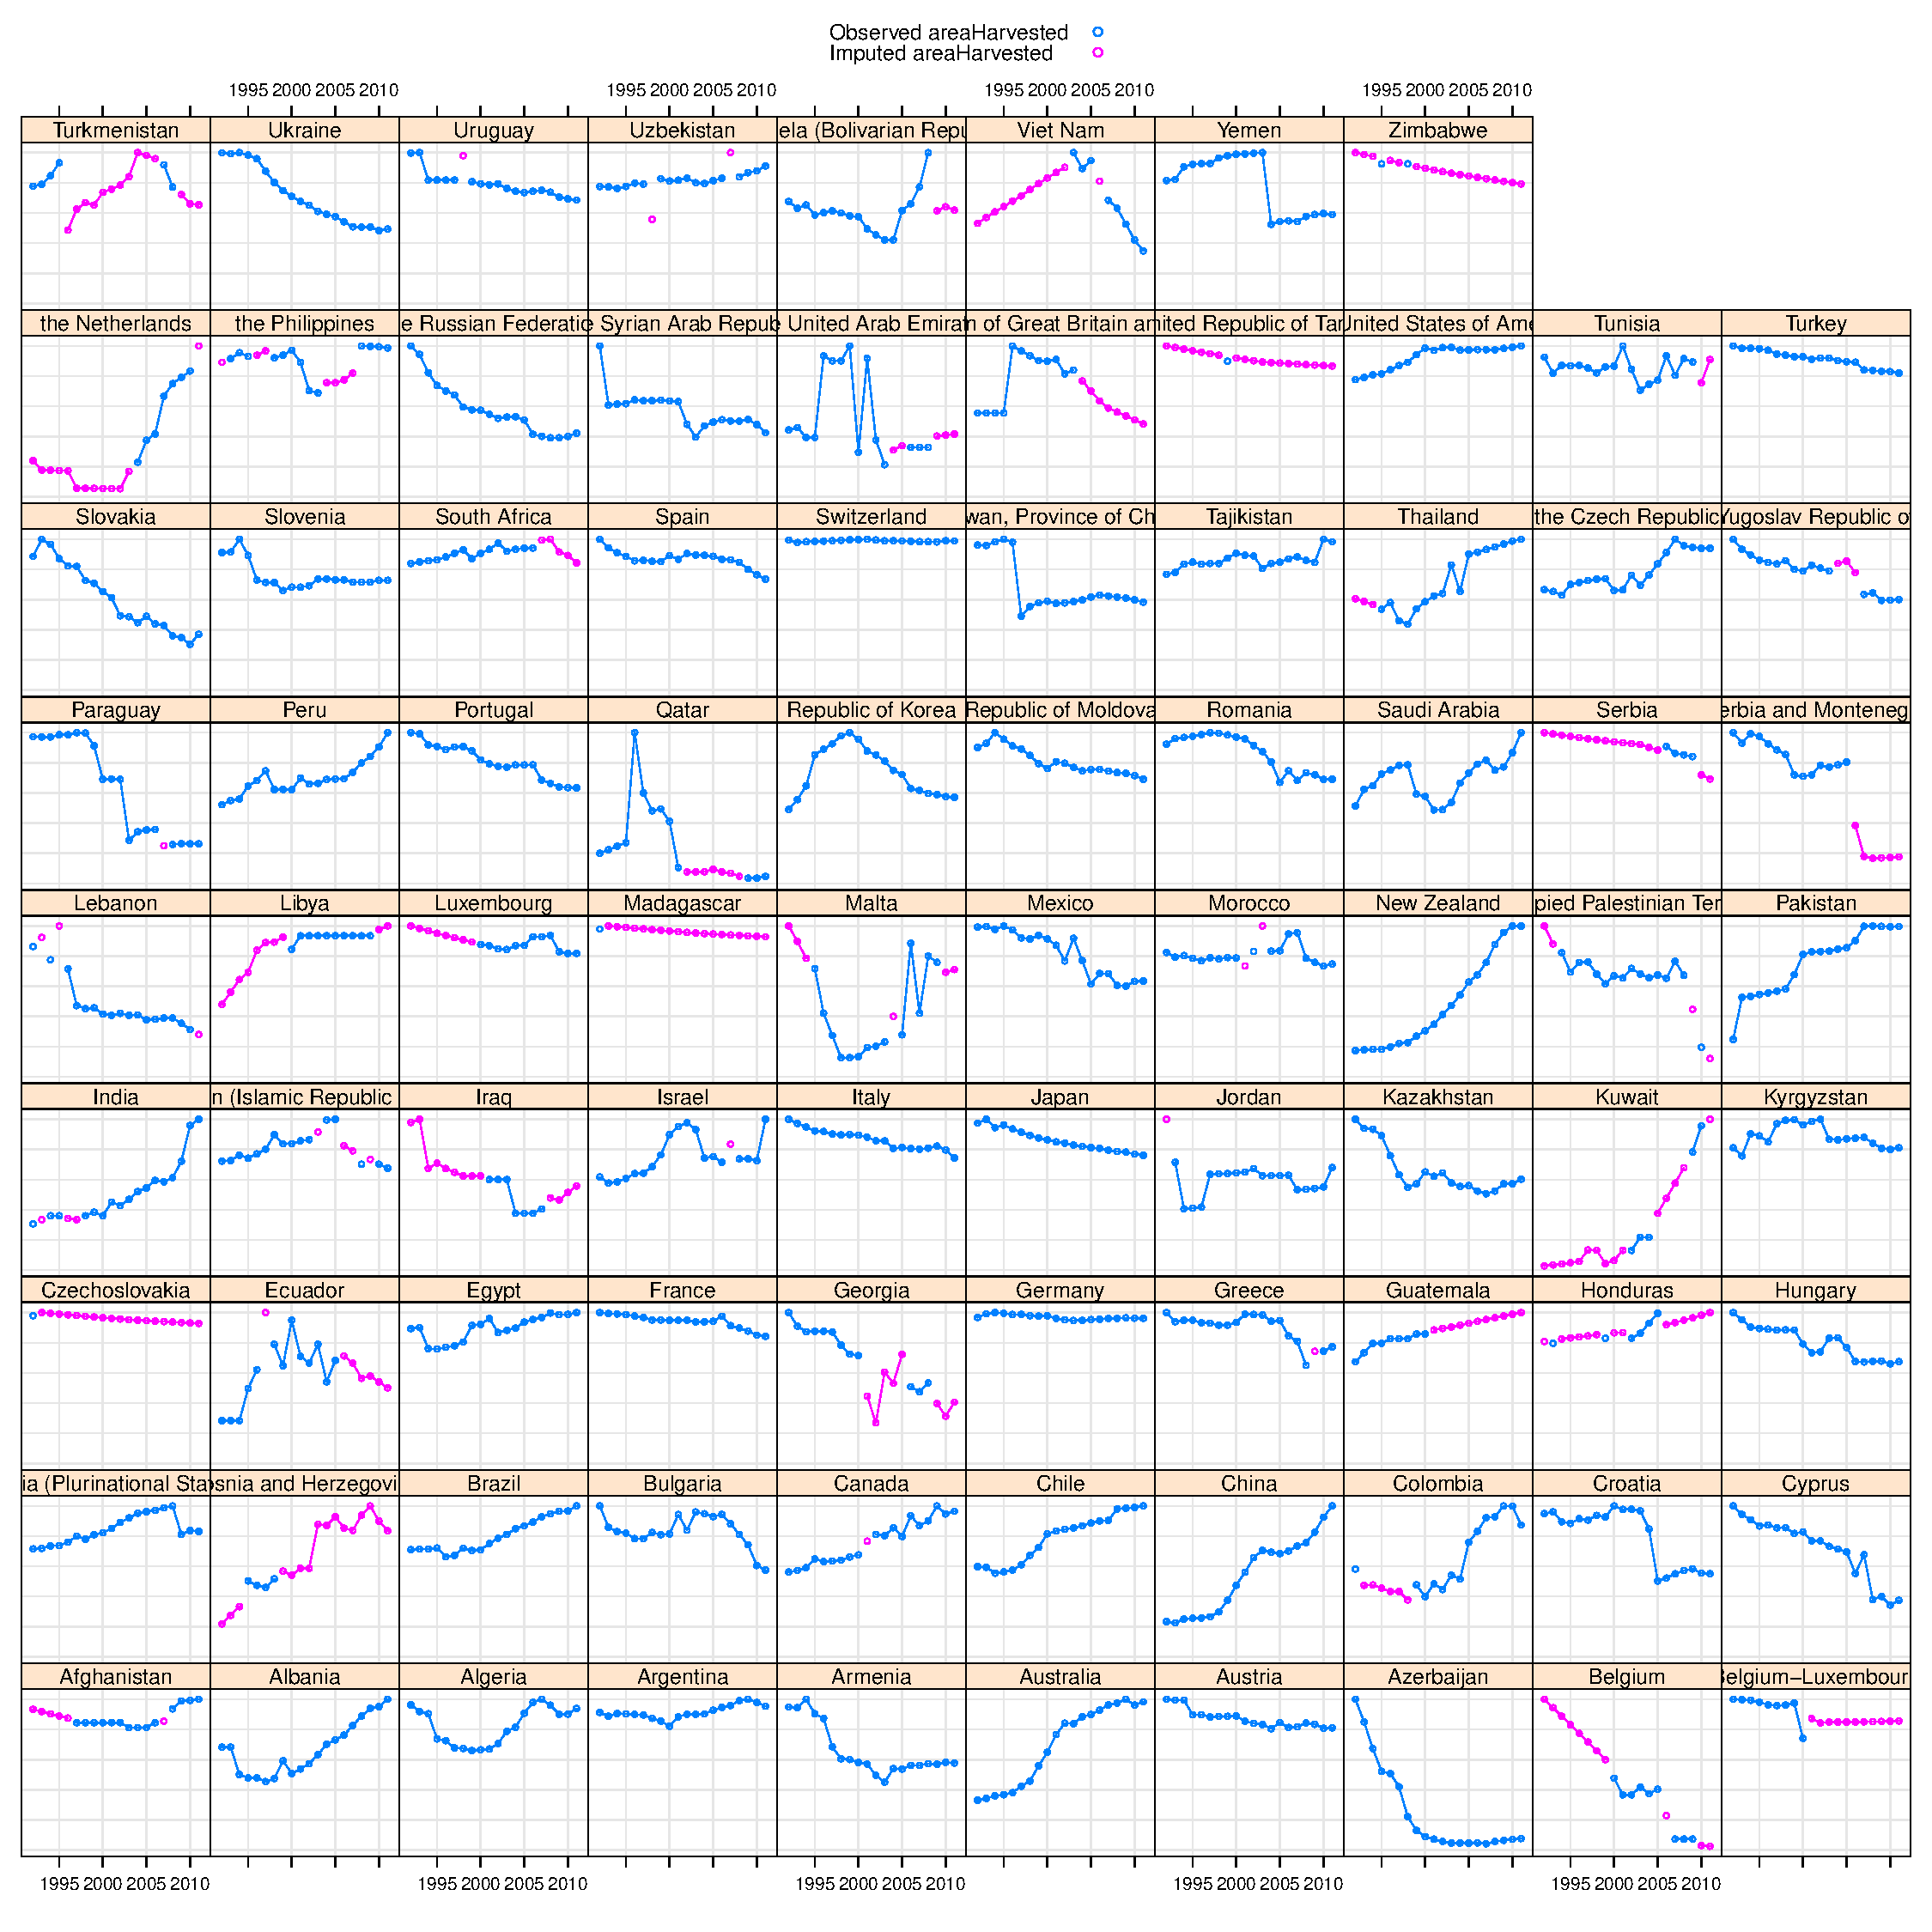
\includegraphics[width=\maxwidth]{figure/grape-areaharvested-imputed} 

}

\caption[Imputation of area harvested of grape]{Imputation of area harvested of grape. The area harvested does appear to be problematic, mostely resembling the trend of the production.\label{fig:grape-areaharvested-imputed}}
\end{figure}


\end{knitrout}



\FloatBarrier
\subsection{Okra}

\begin{knitrout}
\definecolor{shadecolor}{rgb}{0.969, 0.969, 0.969}\color{fgcolor}\begin{figure}[!ht]


{\centering 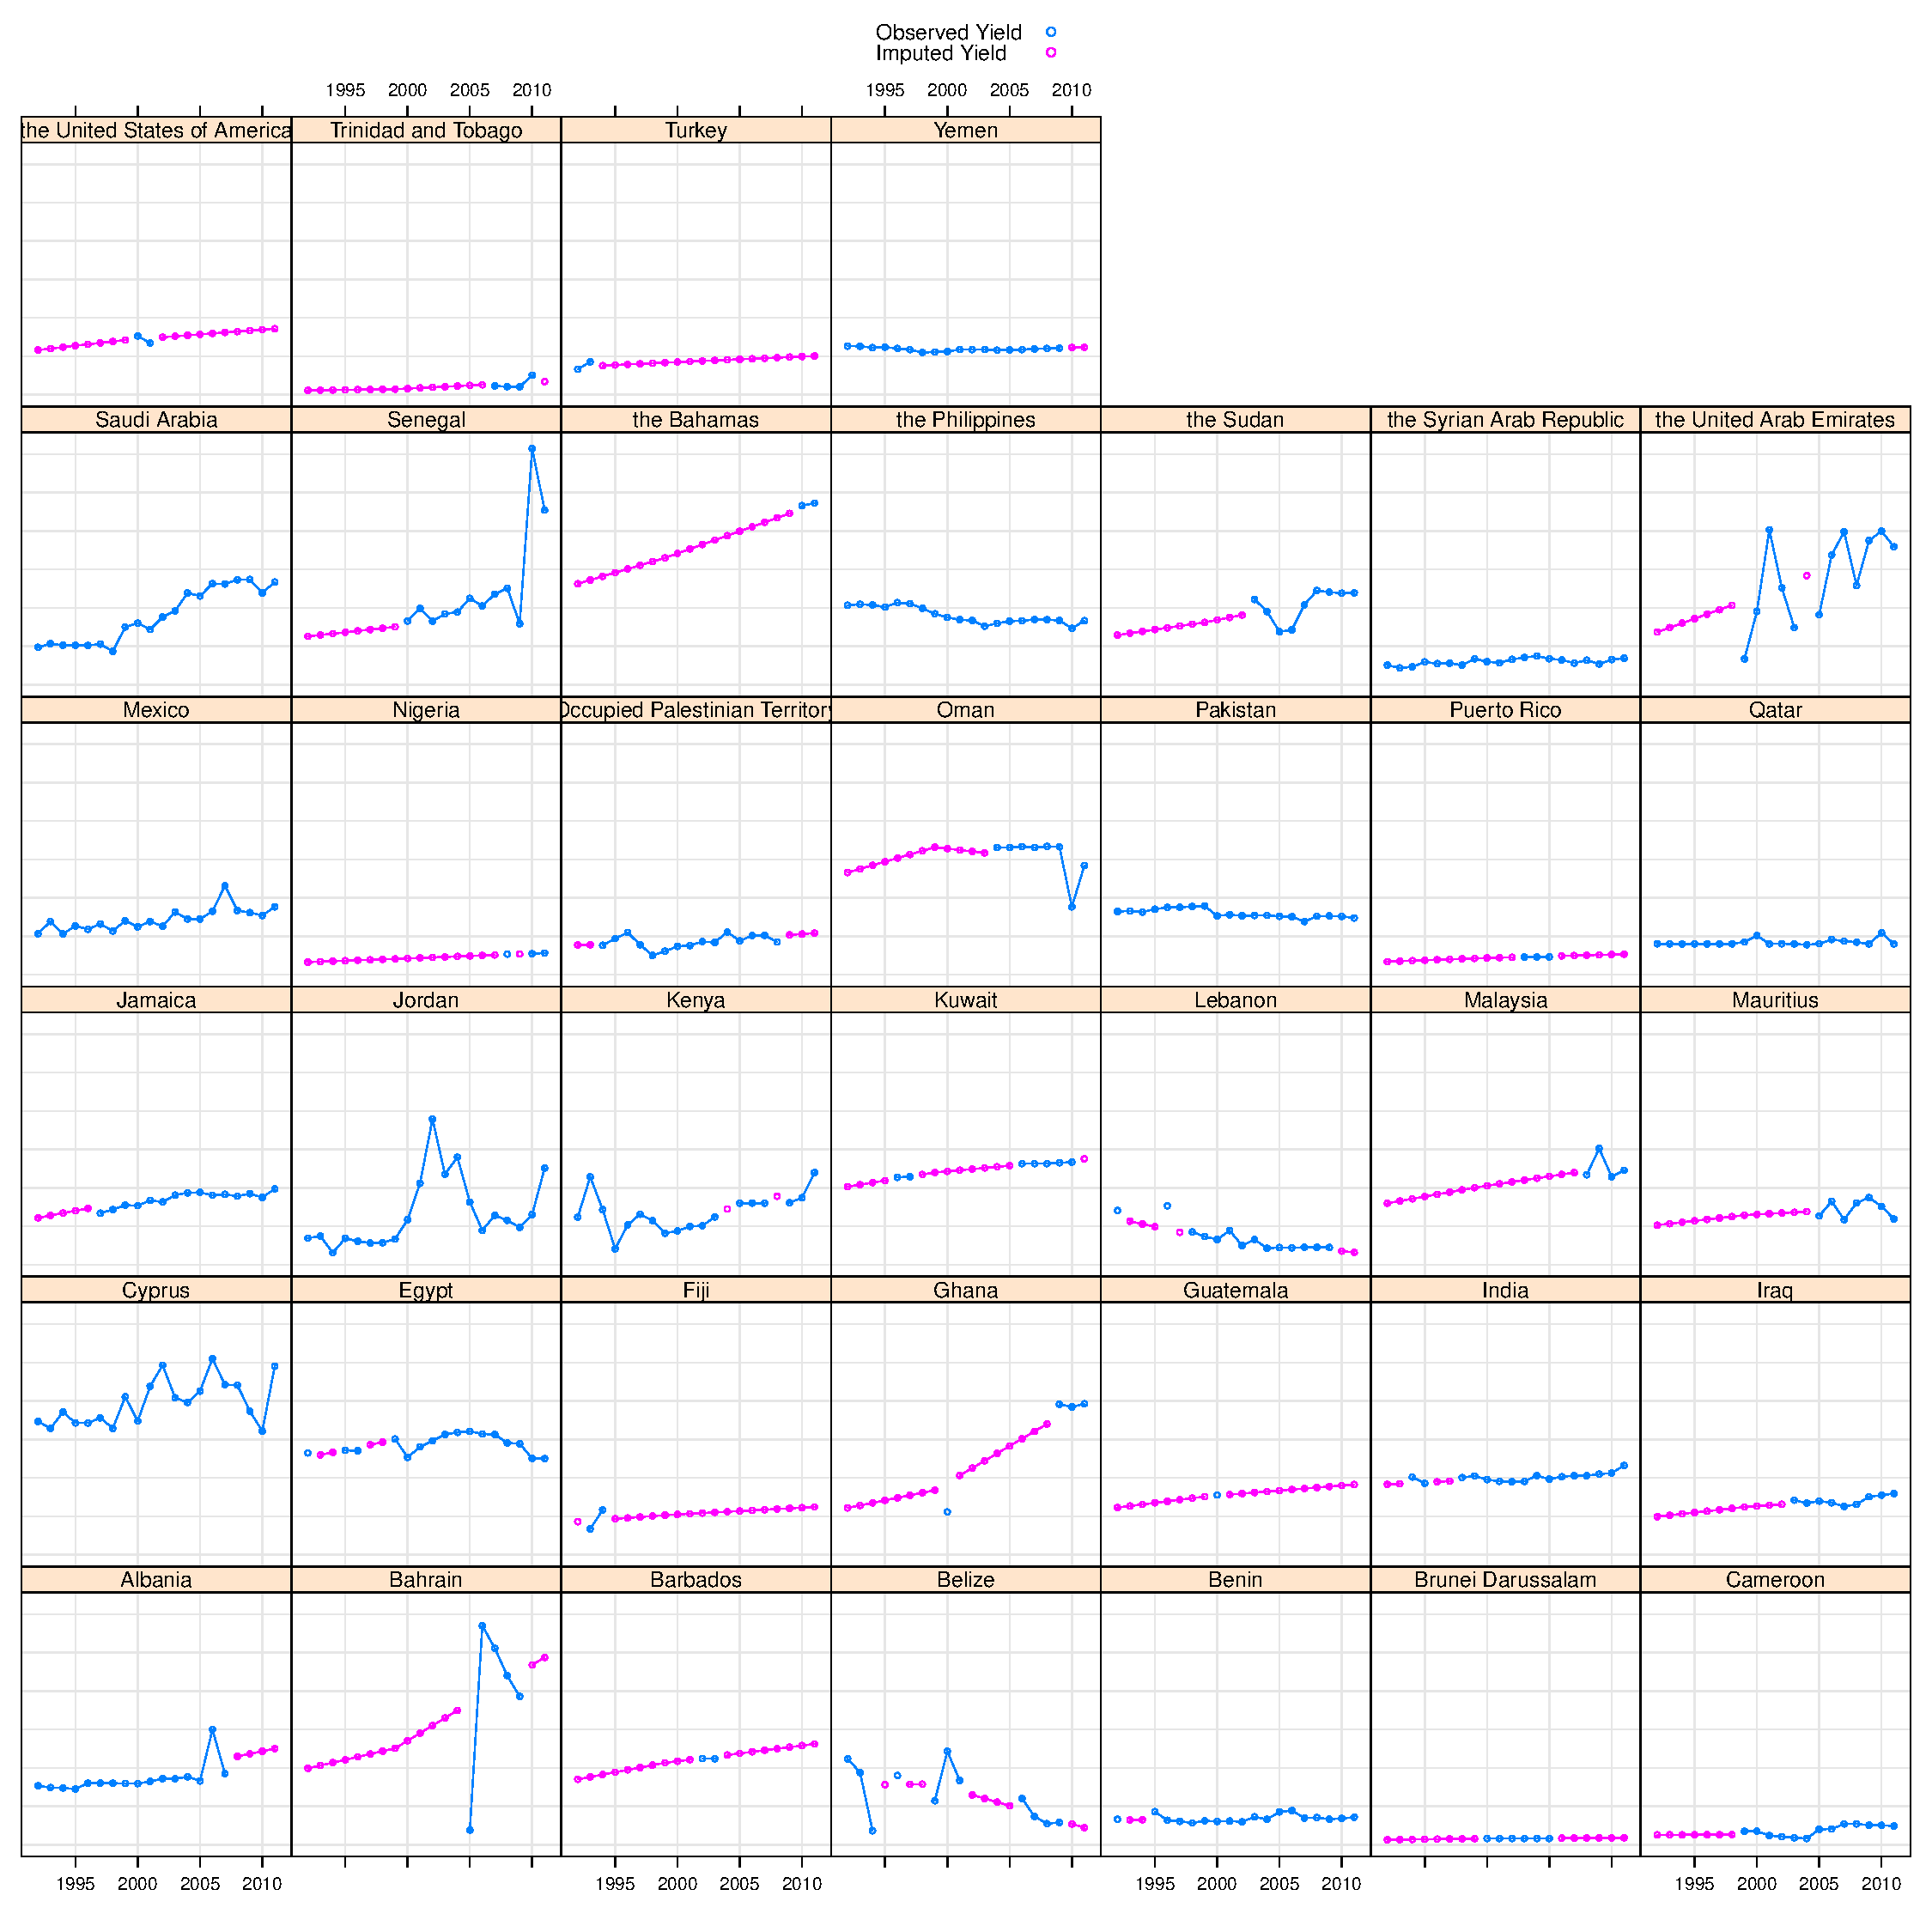
\includegraphics[width=\maxwidth]{figure/okra-yield-imputed} 

}

\caption[The imputation of yield also appears to be reasonable, here once again we see the robustness of linear mixed model not being influenced by the bad data quality of both Senegal and Bahrain]{The imputation of yield also appears to be reasonable, here once again we see the robustness of linear mixed model not being influenced by the bad data quality of both Senegal and Bahrain.\label{fig:okra-yield-imputed}}
\end{figure}


\end{knitrout}


\begin{knitrout}
\definecolor{shadecolor}{rgb}{0.969, 0.969, 0.969}\color{fgcolor}\begin{figure}[!ht]


{\centering 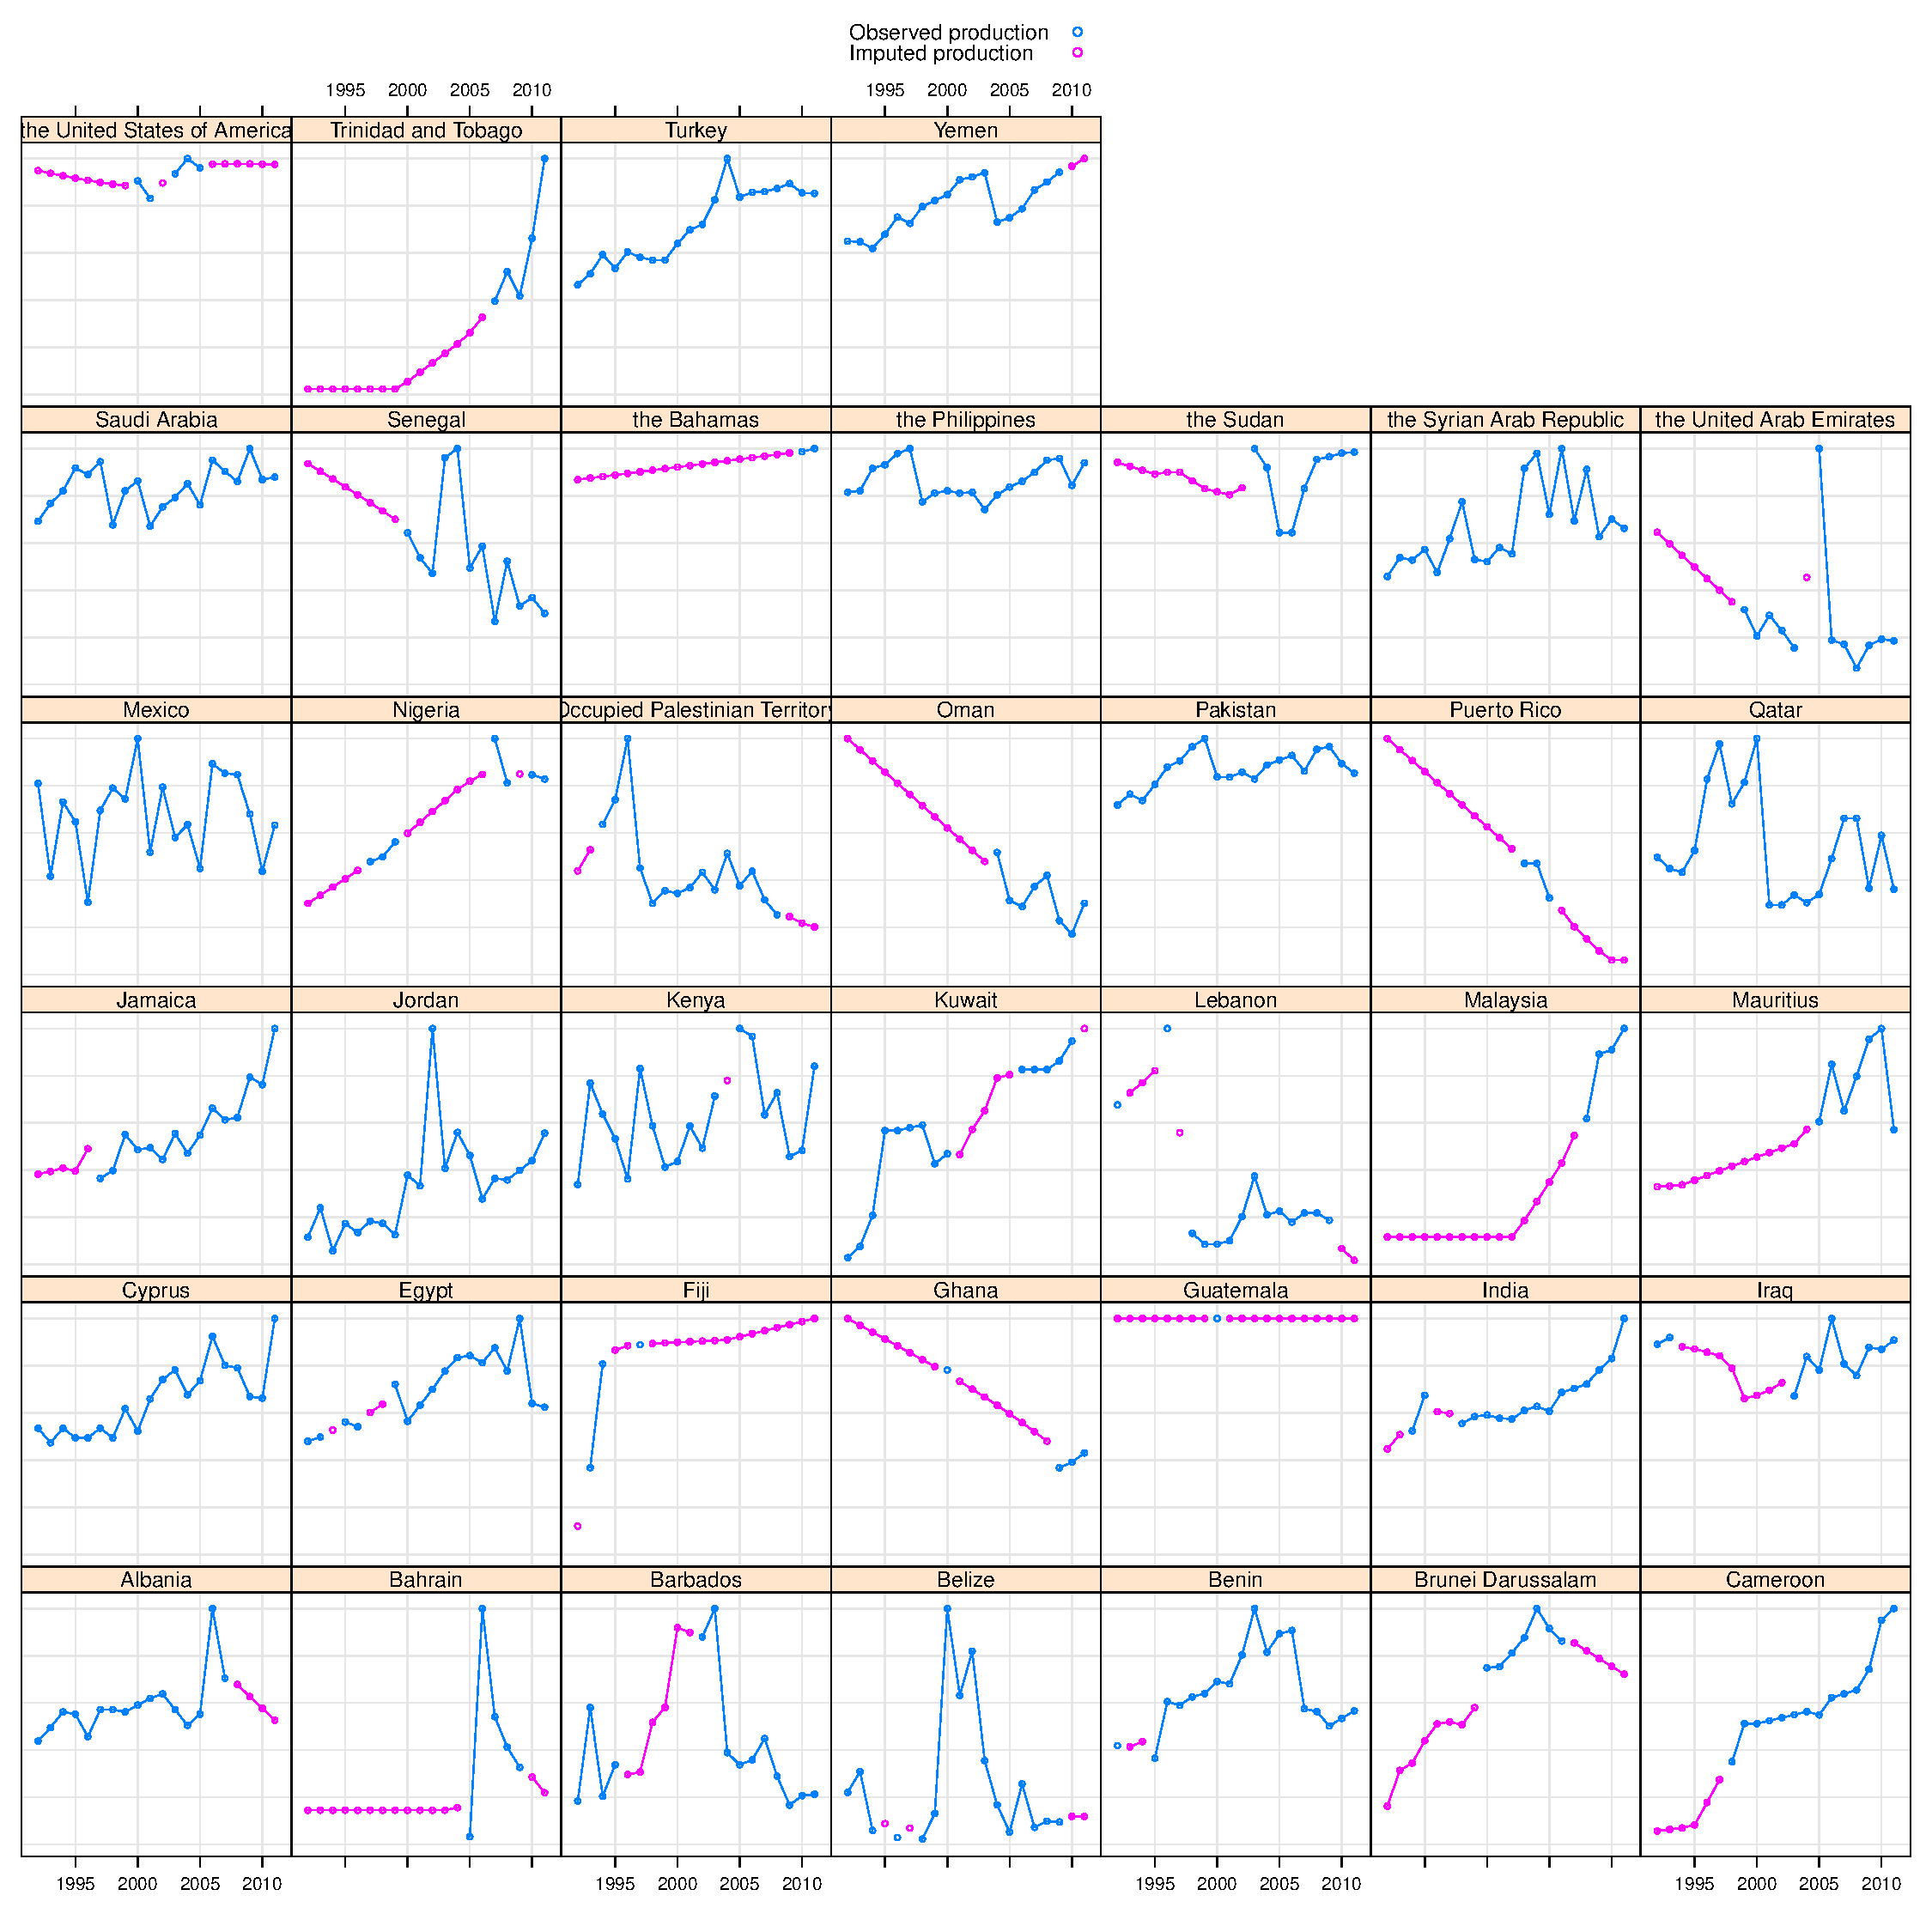
\includegraphics[width=\maxwidth]{figure/okra-production-imputed} 

}

\caption[The imputation of okra prodution]{The imputation of okra prodution.\label{fig:okra-production-imputed}}
\end{figure}


\end{knitrout}

\begin{knitrout}
\definecolor{shadecolor}{rgb}{0.969, 0.969, 0.969}\color{fgcolor}\begin{figure}[!ht]


{\centering 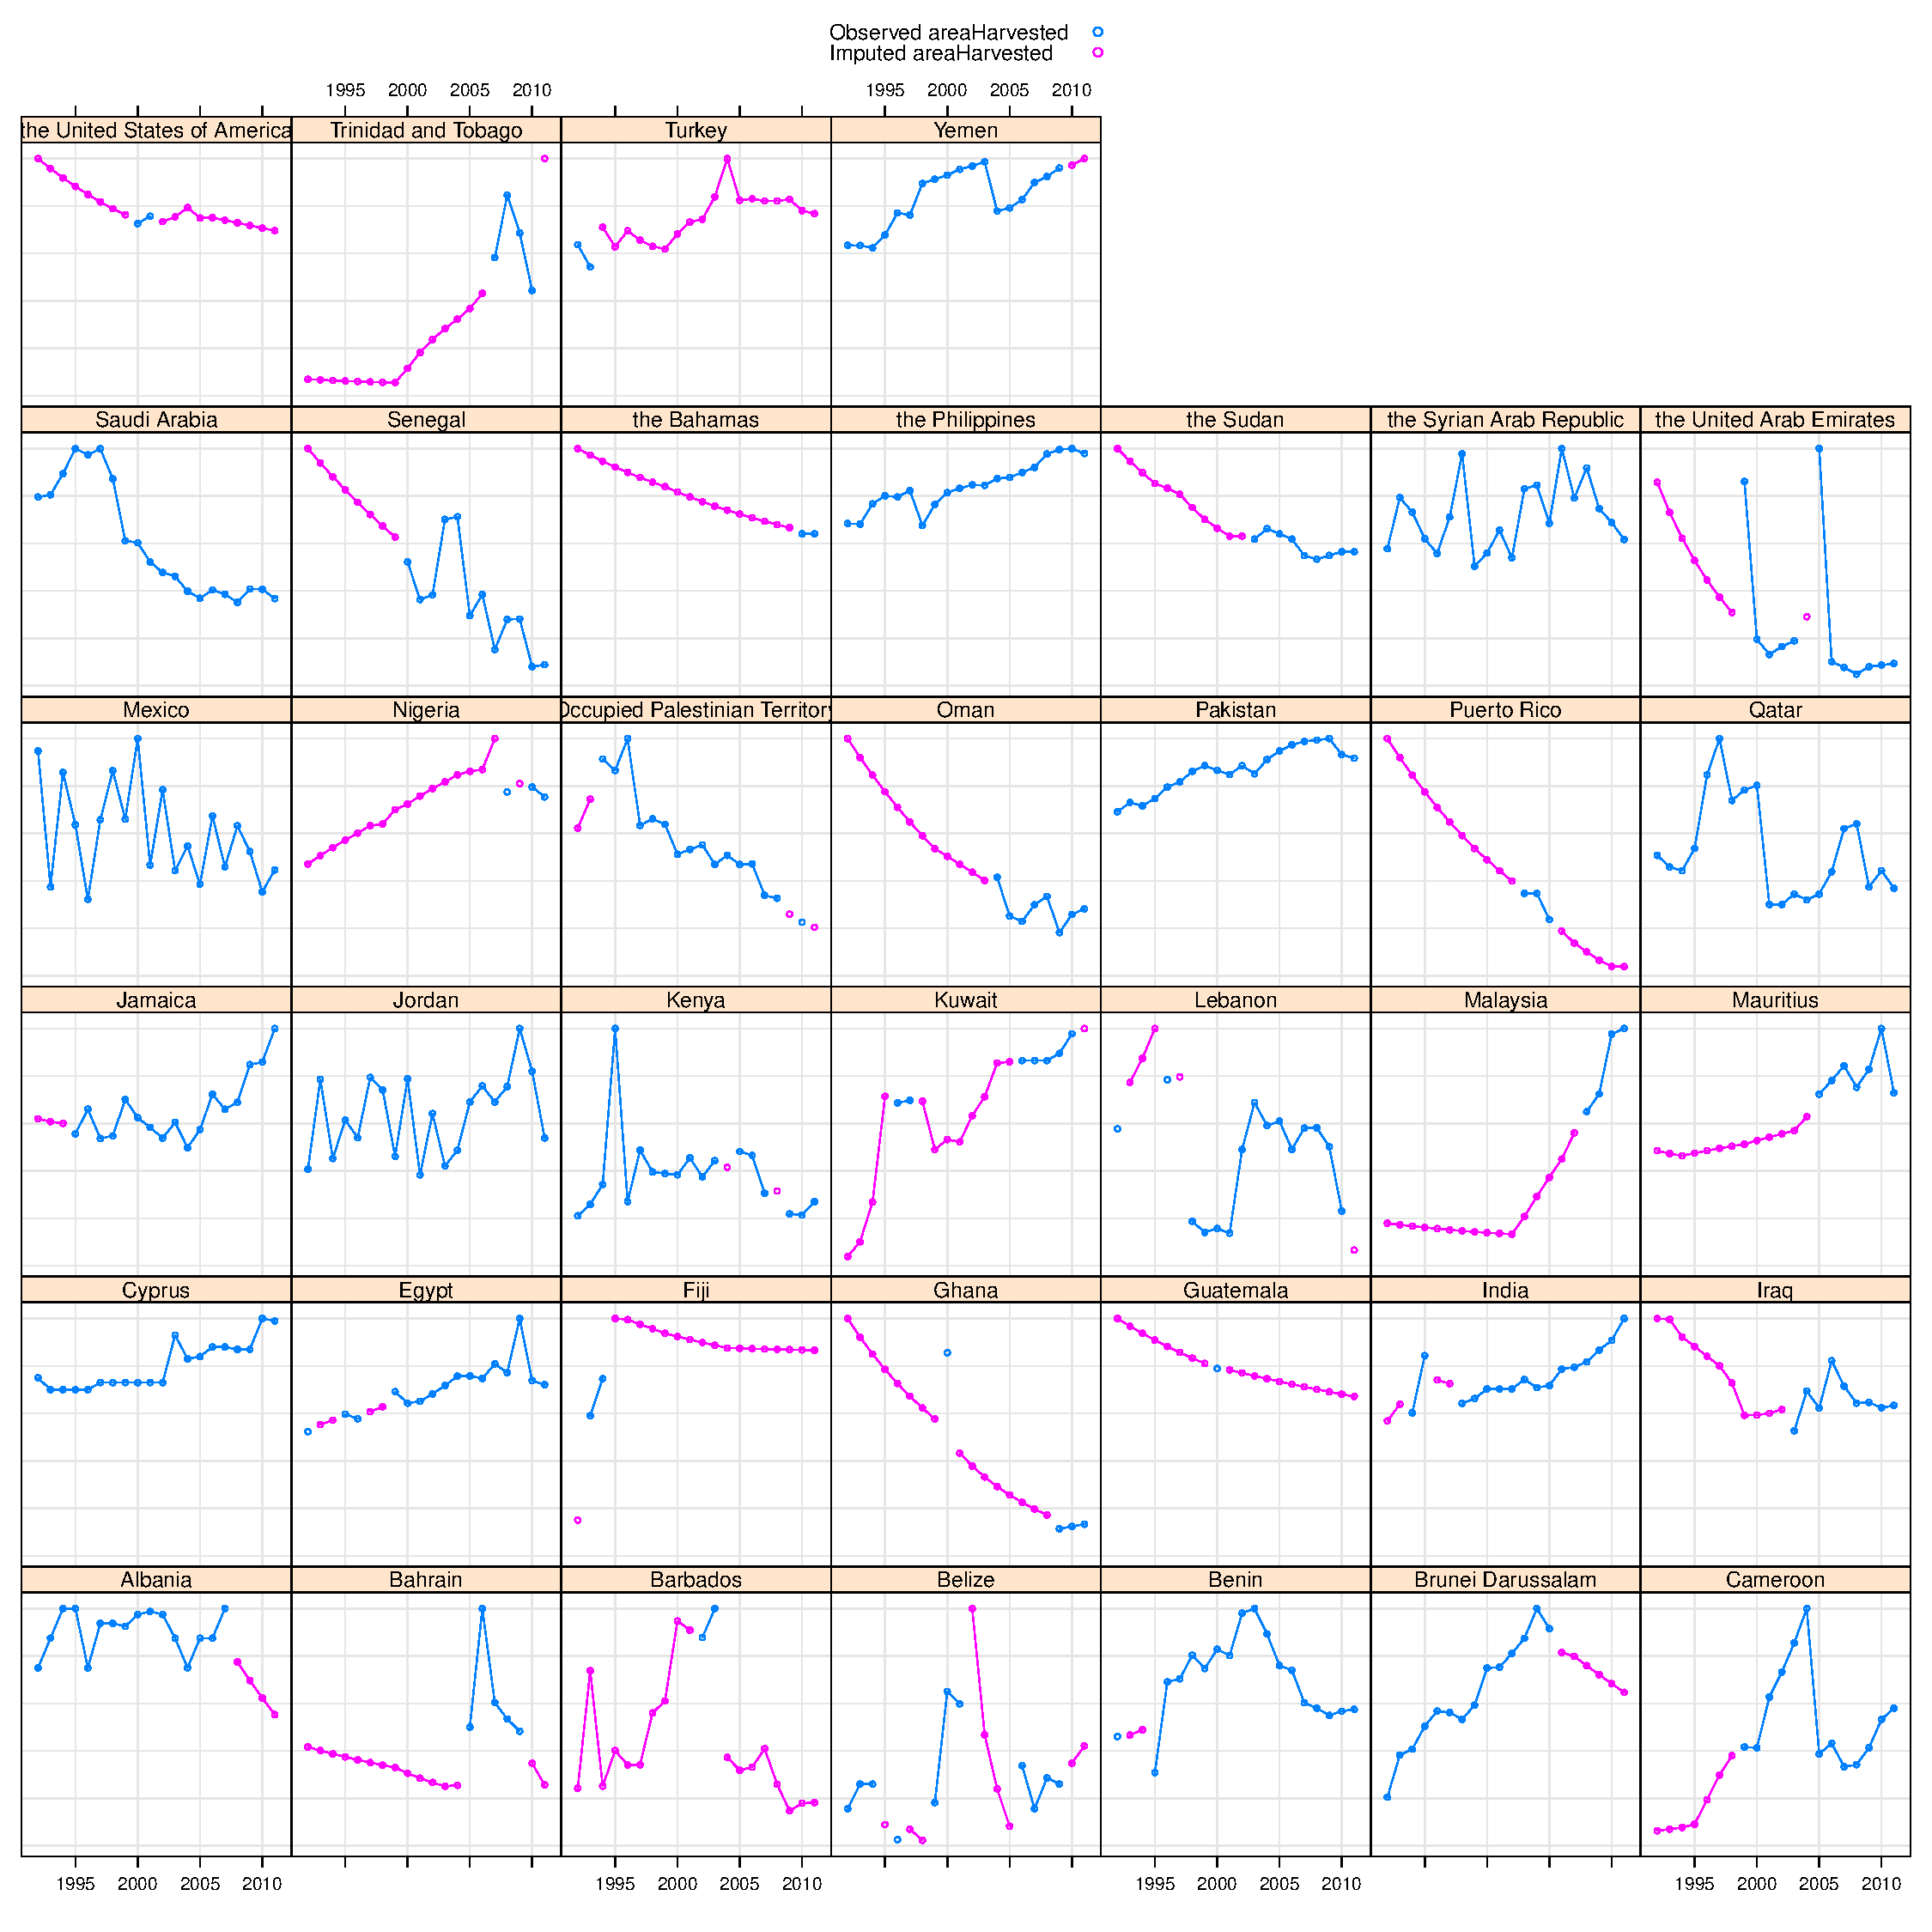
\includegraphics[width=\maxwidth]{figure/okra-areaharvested-imputed} 

}

\caption[Imputation of area harvested of okra]{Imputation of area harvested of okra. The area harvested of Viet Nam does appear to be problematic, the unexpectantly high area harvested is a result of an extremely low yield in the earlier years. This is due to the fact that long extrapolation for over 40 years with only approximately 10 years of data is unreasonable. We can eliminate this problem if we restrict the working data to the past 3 decades.\label{fig:okra-areaharvested-imputed}}
\end{figure}


\end{knitrout}


\FloatBarrier
\subsection{Beef}

\begin{knitrout}
\definecolor{shadecolor}{rgb}{0.969, 0.969, 0.969}\color{fgcolor}\begin{figure}[!ht]


{\centering 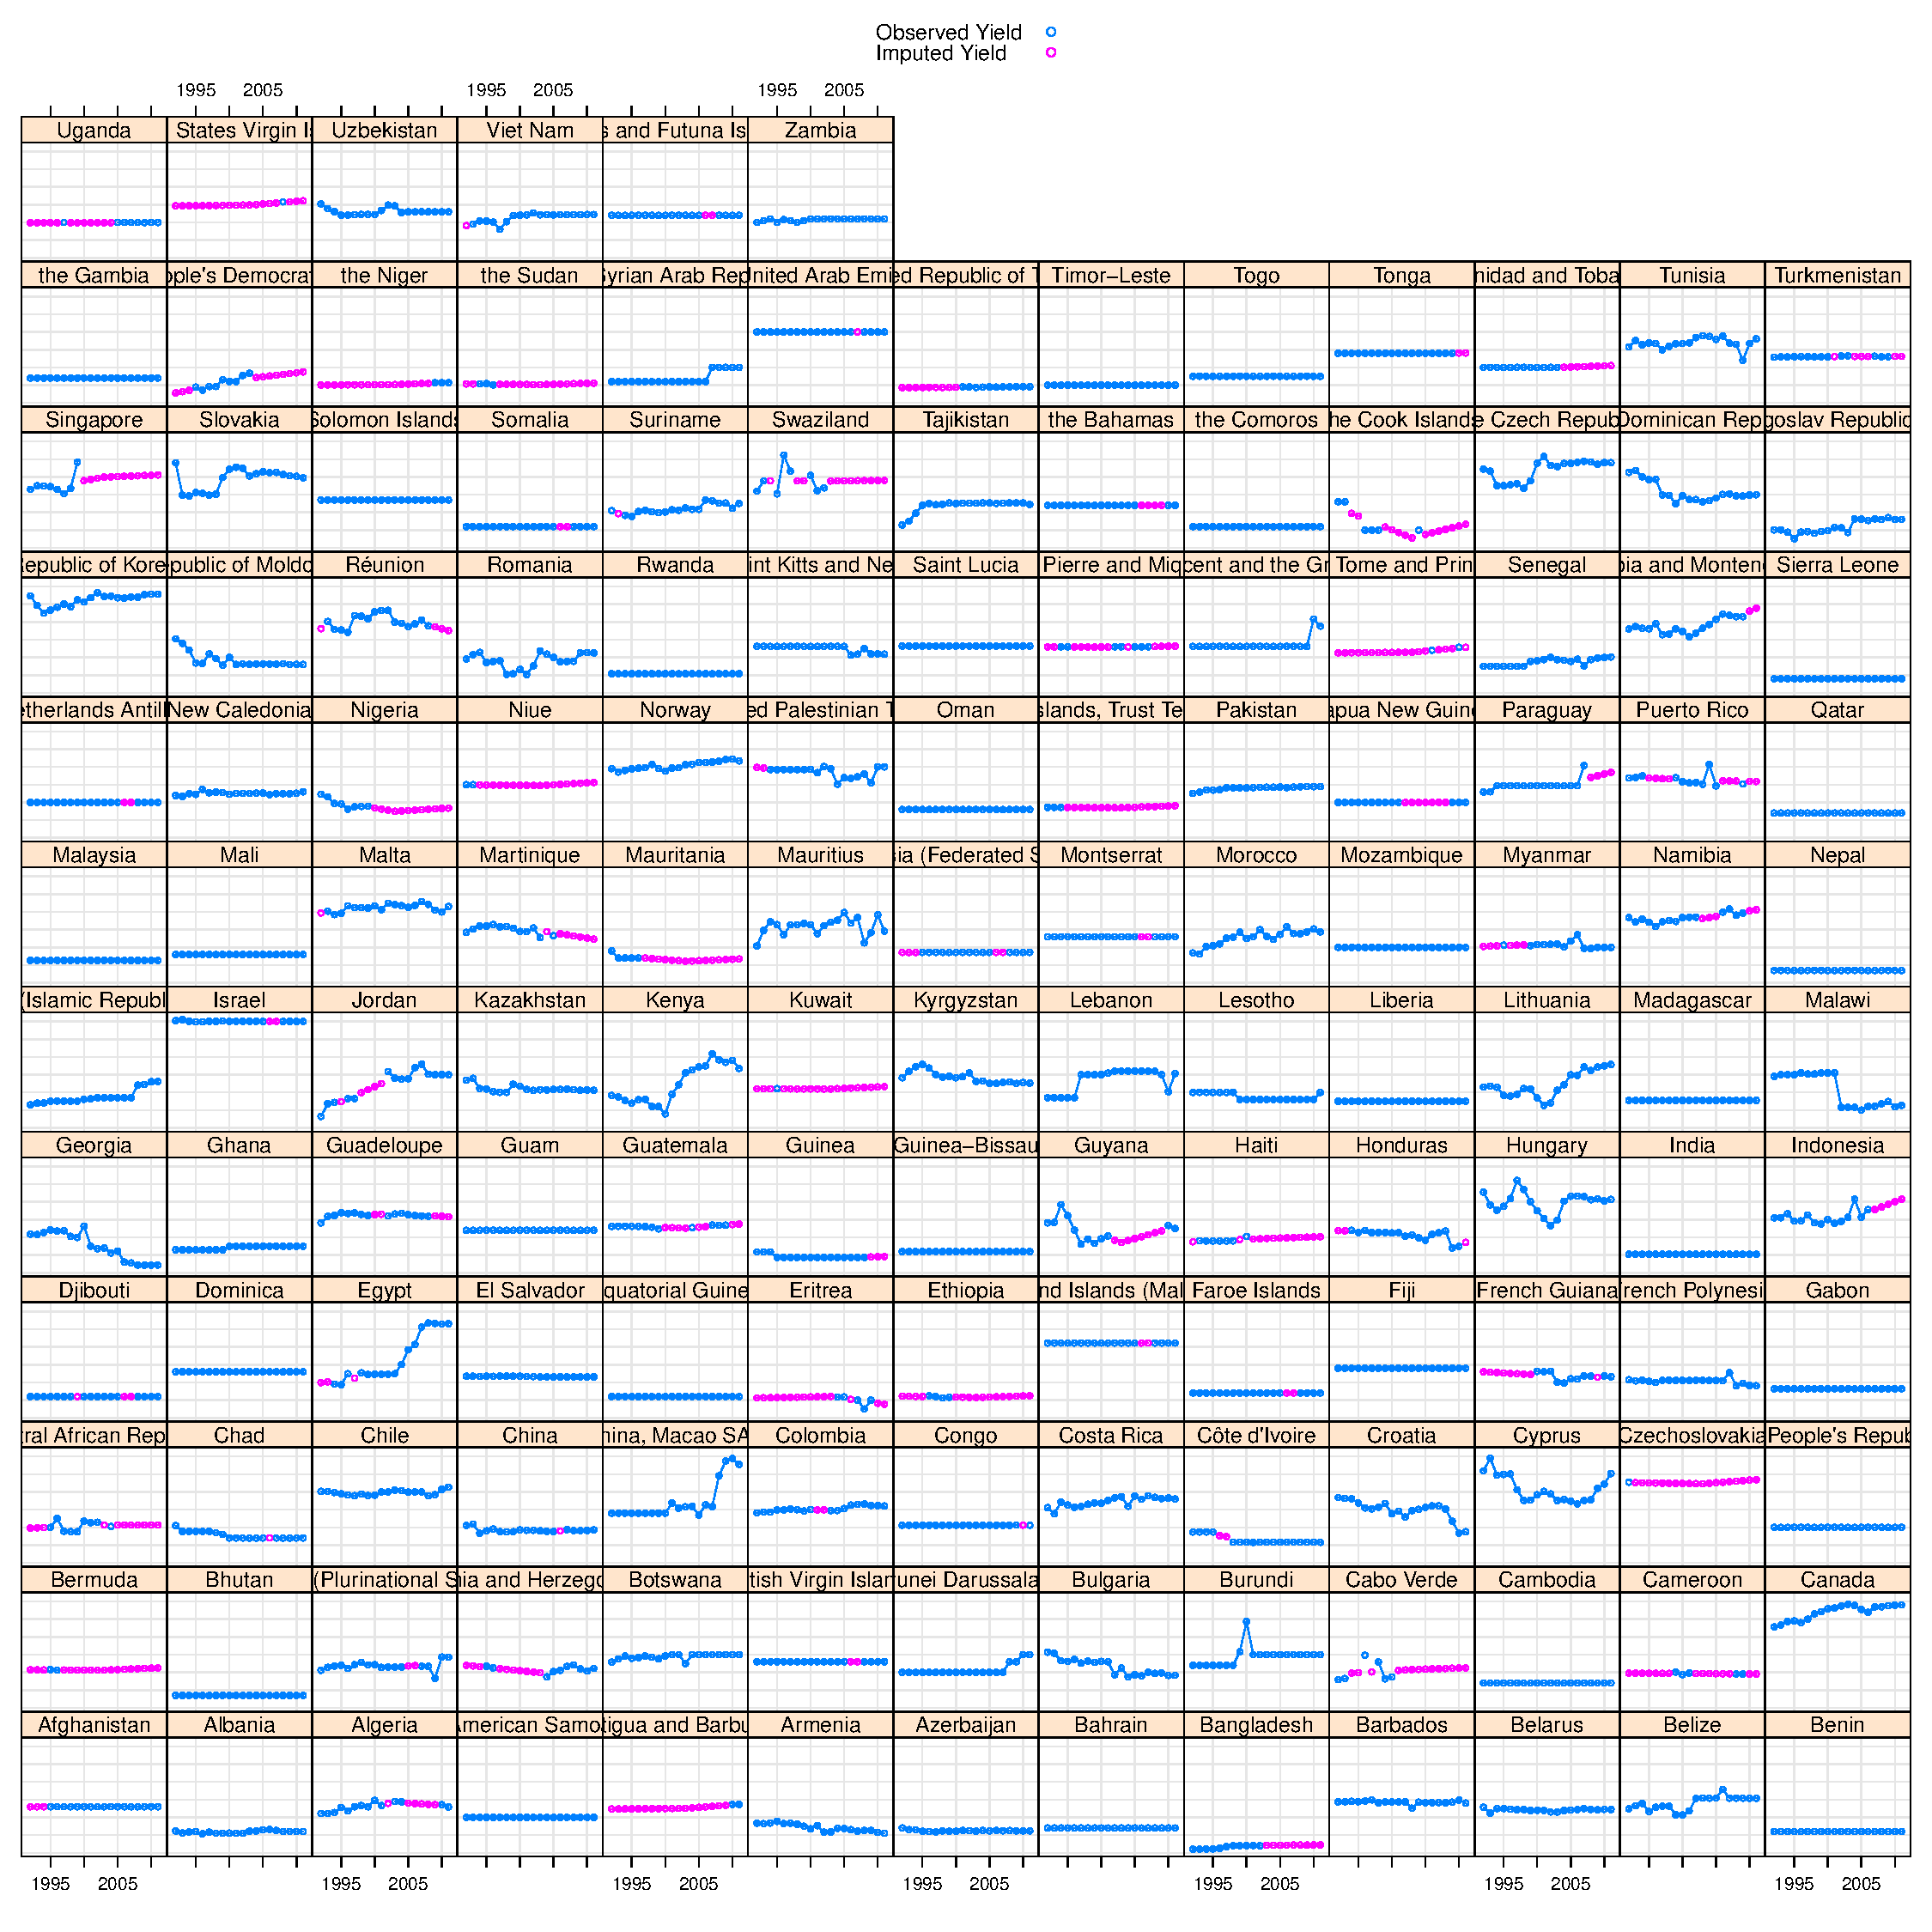
\includegraphics[width=\maxwidth]{figure/beef-yield-imputed} 

}

\caption[Imputation of beef carcass weight]{Imputation of beef carcass weight. .\label{fig:beef-yield-imputed}}
\end{figure}


\end{knitrout}

\begin{knitrout}
\definecolor{shadecolor}{rgb}{0.969, 0.969, 0.969}\color{fgcolor}\begin{figure}[!ht]


{\centering 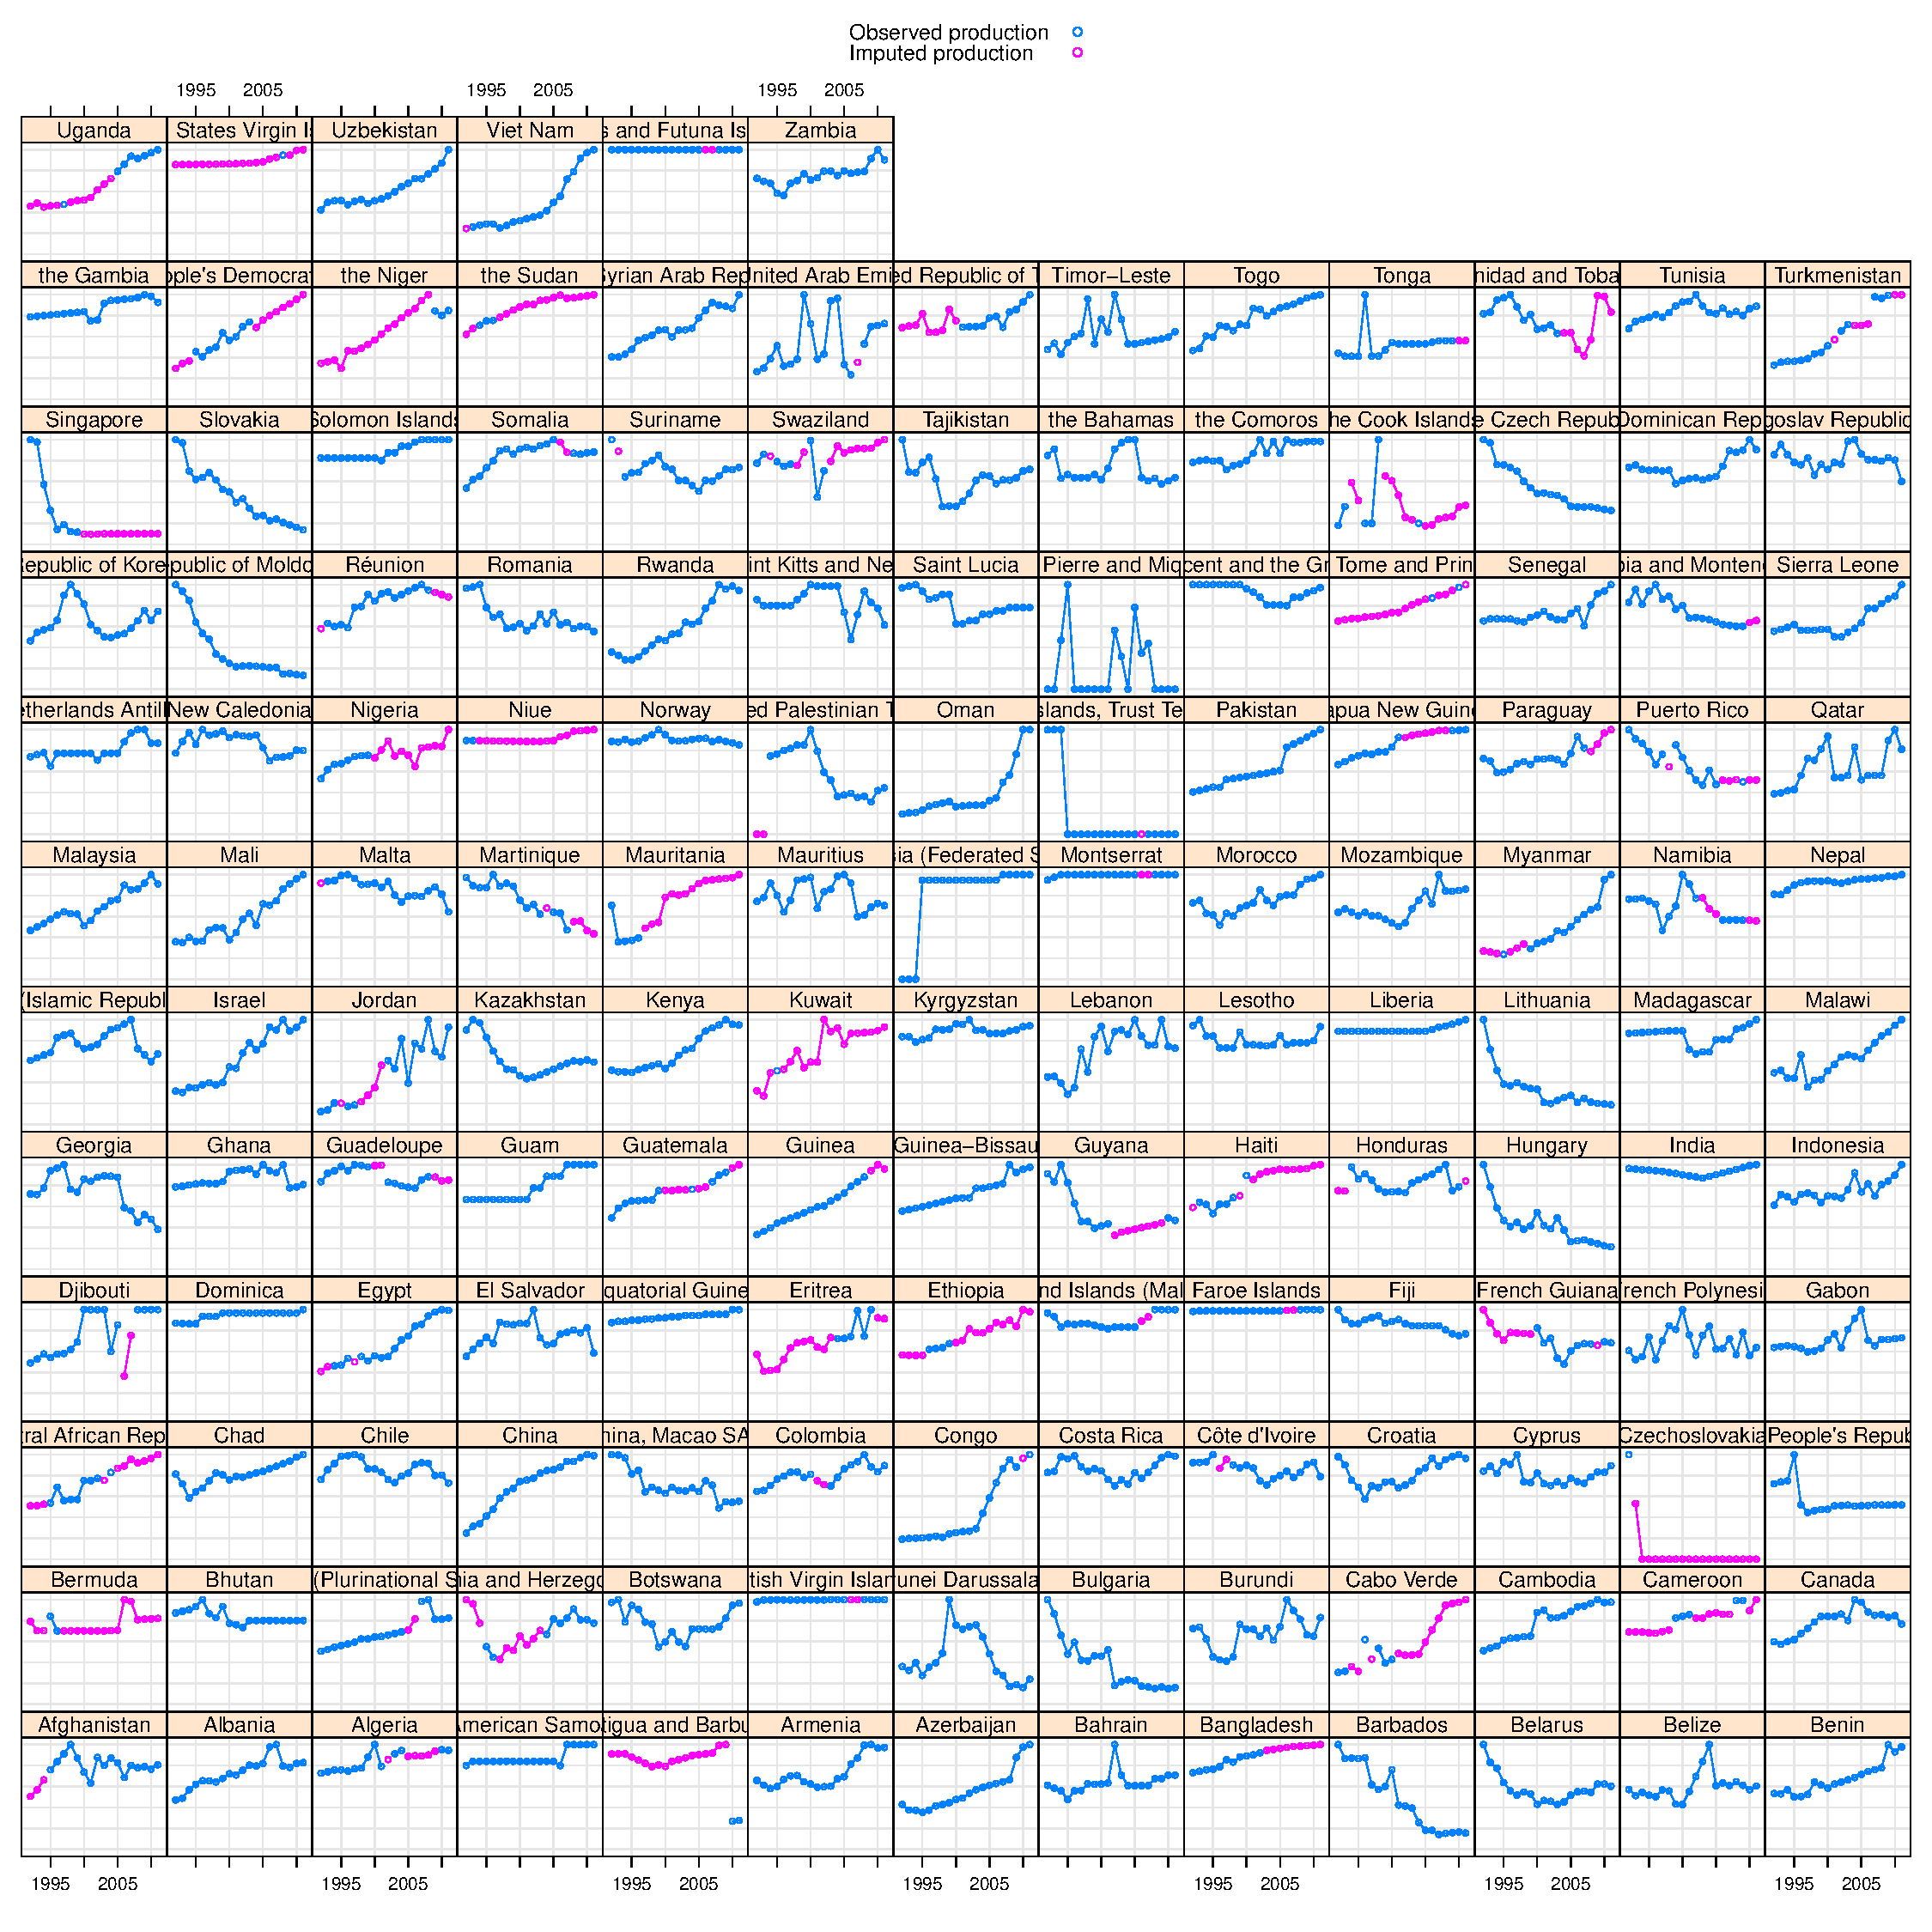
\includegraphics[width=\maxwidth]{figure/beef-production-imputed} 

}

\caption[Imputation of Beef production]{Imputation of Beef production.\label{fig:beef-production-imputed}}
\end{figure}


\end{knitrout}


\begin{knitrout}
\definecolor{shadecolor}{rgb}{0.969, 0.969, 0.969}\color{fgcolor}\begin{figure}[!ht]


{\centering 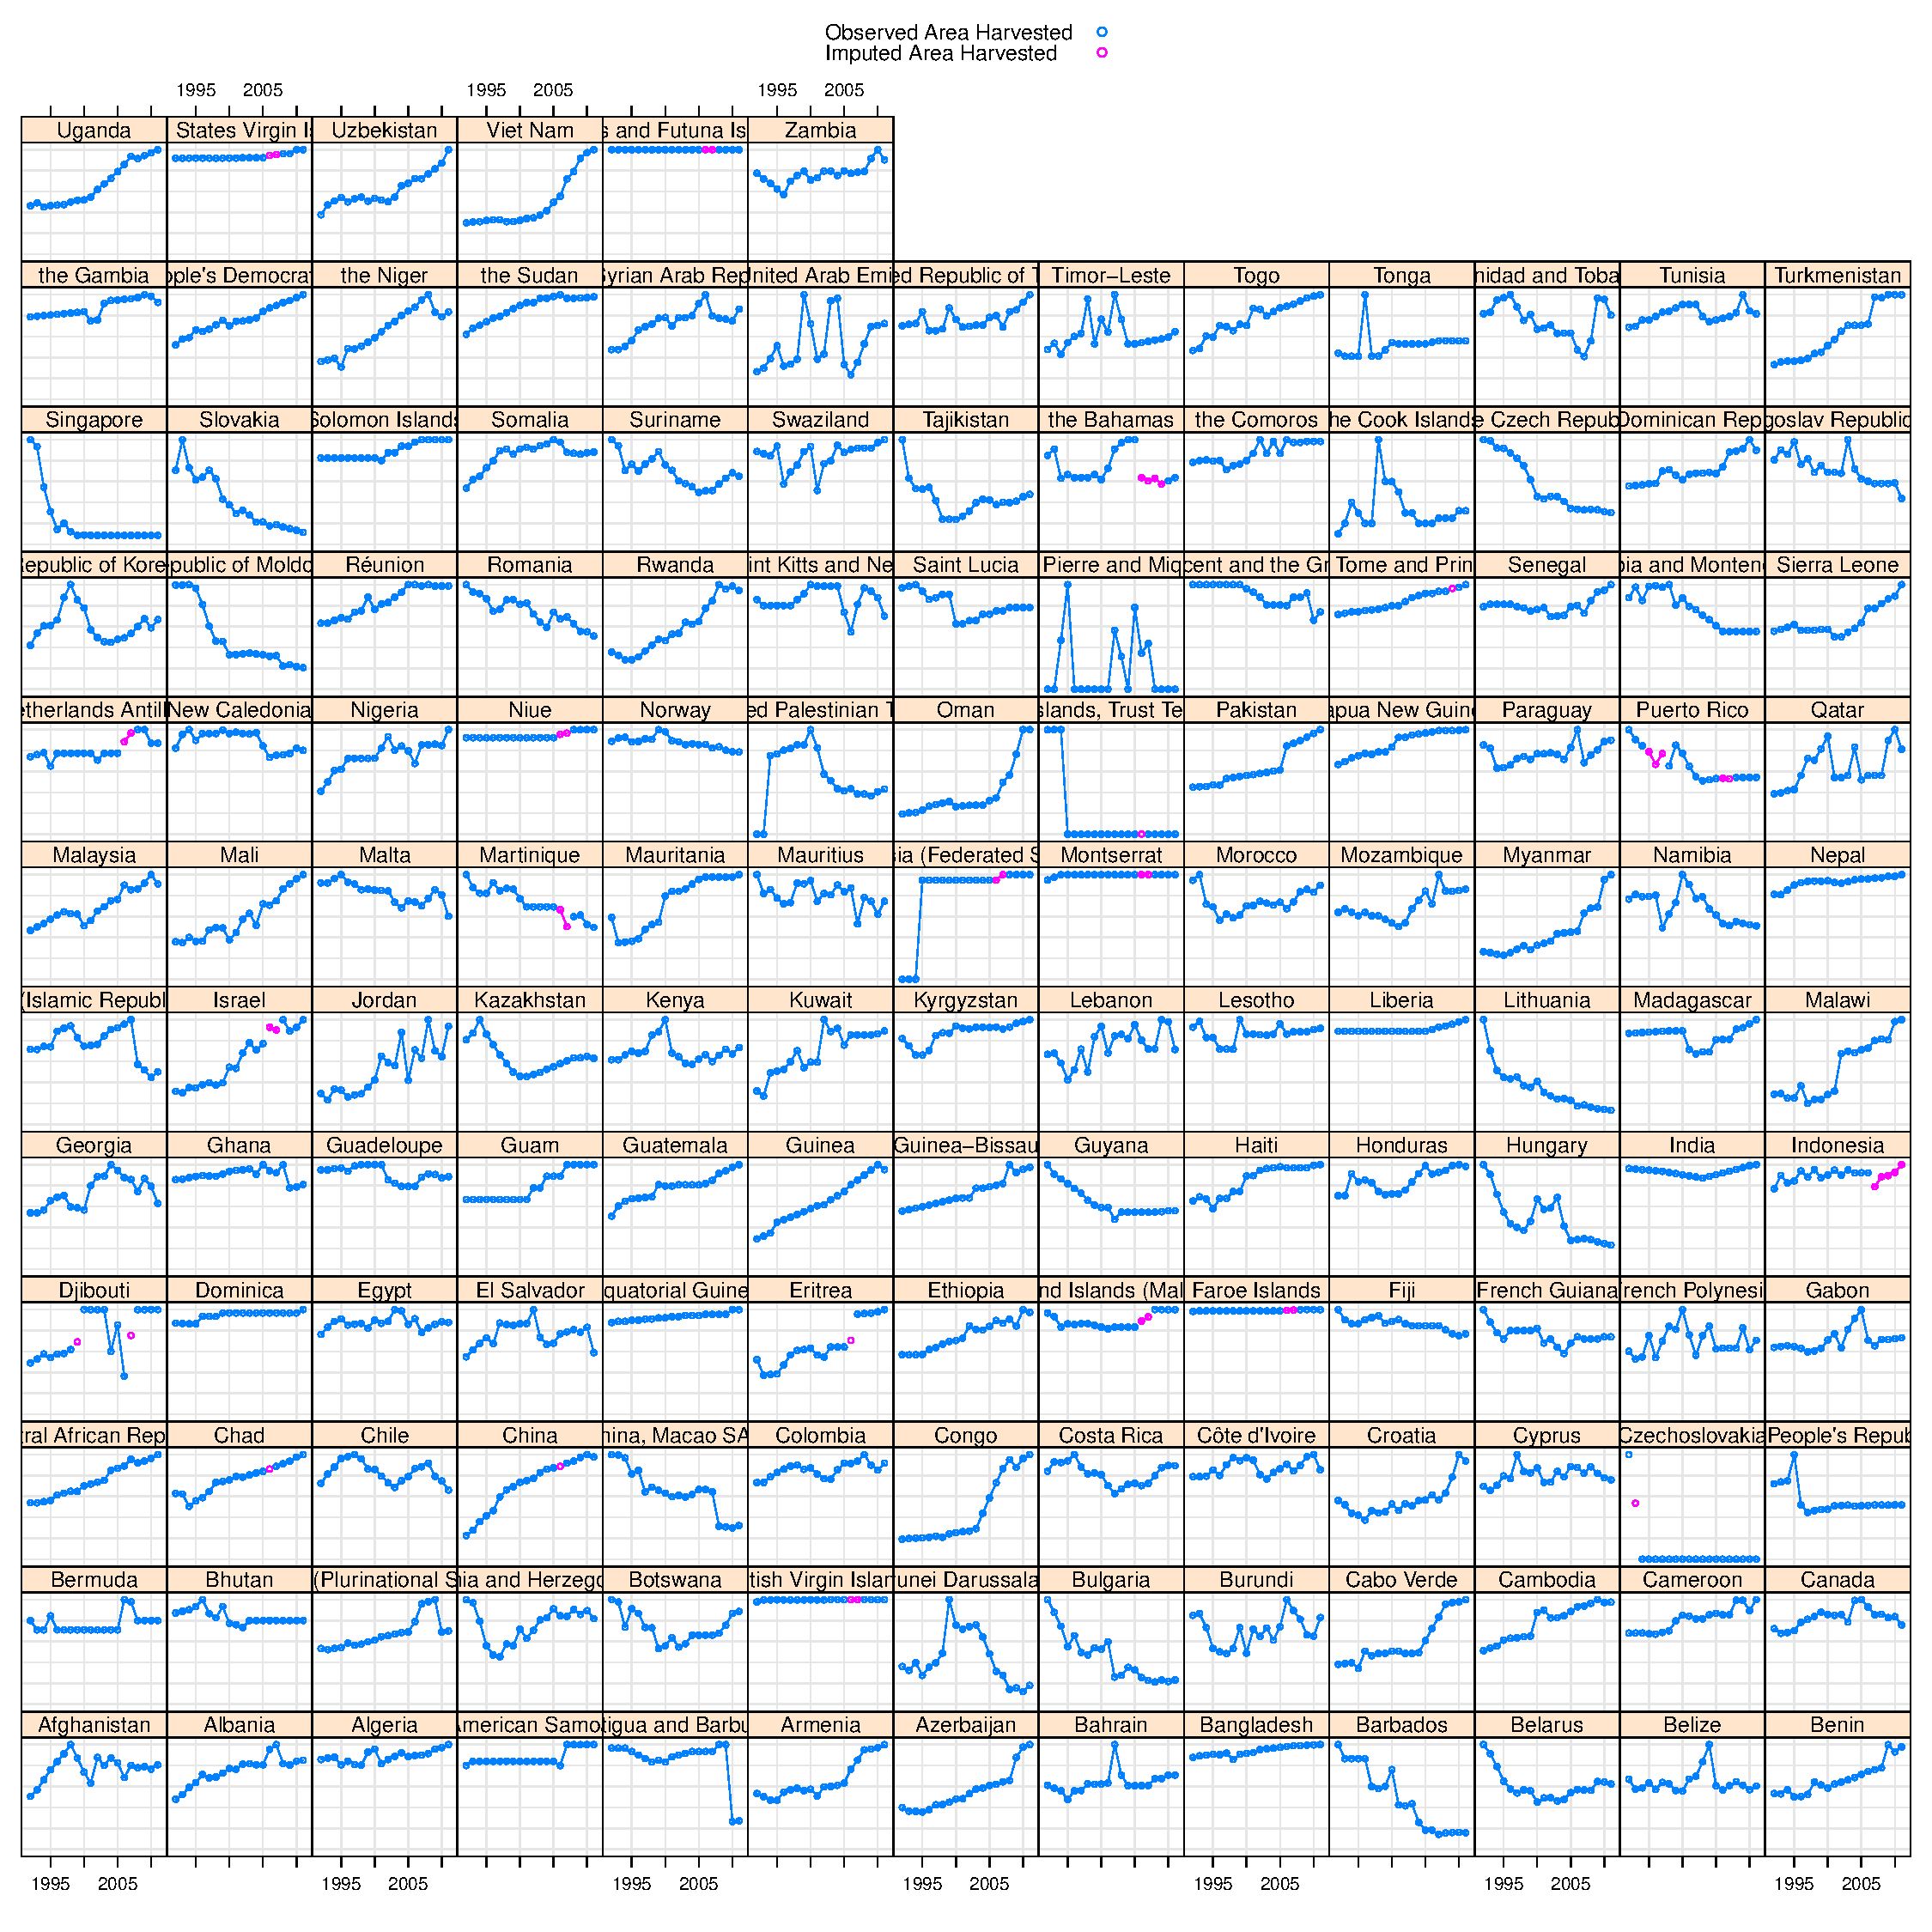
\includegraphics[width=\maxwidth]{figure/beef-areaharvested-imputed} 

}

\caption[Imputation of number of animals slaughtered]{Imputation of number of animals slaughtered.\label{fig:beef-areaharvested-imputed}}
\end{figure}


\end{knitrout}








\FloatBarrier

From the case studies, we can see that we have an extremely flexible
model with almost no possibility of over-fitting since none of the
model are itself complex. The model is robust as a result of the
variance reduction property of ensemble and even in cases where we
have extremely sparse data we can still fall back to simpler models
with fewer assumption.\\


The model is not only flexible in adapting to change in the data
generating mechanism, but at the same time flexible to accommodate
further models in which we consider appropriate. Any model which
offers diversity and additional predictive power can be included to
further enhance the ensemble.\\


\FloatBarrier
\section{Simulation Styudy}

In order to understand the performance and characteristics of the
imputation, we have conducted simulation to estimate the prediction
error of the imputation.\\

For each bootstrap, we take a sample containing only official and
semi-official data and impute the values which are missing. The
imputation is then benchmarked with the actual observed official and
semi-official data. We use the Mean Absolute Percentage Error (MAPE)
for assessing the accuracy of the imputed values; and we compute the
coverage rate defined as the proportion of missing value imputed to
examine the applicability of the method.

\begin{equation}
  \text{MAPE} = \frac{1}{N} \sum \left|\frac{y_i -
    \hat{y}_i}{y_i}\right|\\
\end{equation}


Each simulation draws a sample of varying missing proportion, this is
to investigate the prediction error over different degree of
missingess and at the same time to detect the breaking point of the
method.\\

Since there are already missing value in the data, the benchmark is
can only be computed on the available official and semi-official data
which varies between commodity. We have over 70\% availability of
benchmark observations for wheat, while only slightly over 20\% for
pepper.\\


Here is the table for the result of the simulation, 50 boot strap
samples were drawn for each scenario. The final percentage error is
calculated as the average of all the bootstrapped error within the
group. The missing percentage for grapes and beef were higher than
20\% already and thus a simulation was not possible for the group of
20\% missing proportion.

\begin{table}
  \centering
  \label{tab:simResult}
  \caption{Simulation result for the imputation methodology.}  
  \begin{tabular}{|c|c|c|c|}
    \hline
    Commodity & Total Missing Proportion & Effective Missing Proportion & MAPE (\%)\\
    \hline \hline
    \multirow{4}{*}{Wheat}
      & 30.9\%  & 20\% & 3.68\\
      & 48.1\%  & 40\% & 7.84\\
      & 65.4\%  & 60\% & 13.01\\
      & 82.7\%  & 80\% & 25.19\\
    \hline
    \multirow{4}{*}{Grapes}
      & 39.5\%  & 20\% & 4.49\\
      & 54.6\%  & 40\% & 9.31\\
      & 69.7\%  & 60\% & 14.63\\
      & 84.9\%  & 80\% & 21.69\\
    \hline
    \multirow{4}{*}{Beef}
      & 57.4\%  & 20\% & 1.04\\
      & 68.1\%  & 40\% & 2.32\\
      & 78.7\%  & 60\% & 4.15\\
      & 89.4\%  & 80\% & 7.67\\
    \hline 
  \end{tabular}
\end{table}


\FloatBarrier
\section{Conclusion}

In this paper, we have proposed a new complete framework to impute the
production domain which encompase the production, area harvested and
yield. Due to the size of the project scope, flexibility and
robustness were essential elements of the model developed.

Demonstration shows that the two proposed models tailored were
successful in solving problems faced by previous methodology. The
linear mixed model for spline allows historical trend, cross-country
and cross-commodity information to all be utilized. Further, the
pooled information also enpowered the model to be safe-guarded by
outliers observed in the data. The ensemble tackles the problem in an
entirely different way as the correlation structure and behaviour does
not resemble those of the yield. Yet, the result is the same, model
were robust and flexible to accommodate anything from a simple trend
to complex time series.

Despite the outcome seemingly promising, there are still shortcomings
in the model. The proposed linear mixed model for yield does not have
the ability to seize the year-to-year variation displayed. Further,
the three variables are still modelled separately. A fully integrated
framework which models the whole identity equation is desirable.


\section{Further Improvements}
An ongoing project is dedicated to the designation of weights
reflecting the information content of the observations. Data collected
from official and semi-official sources may be deems as more reliable
while observation from expert judgement may be less reliable. A
weighting scheme will allow the models to better assess the quality of
information and improve the performance.\\

Further, to capture the year-to-year variation of the yield, a pilot
experienment for utilizing remote sensing data is tested. The
temperature and precipitation published by the World Bank does not
have both the temporal and spatial resolution to accurately estimate
the variation. We are making an attempt to match the precipitation and
teperature to specific crops by combining information from satelite
images of Normalized Differenced Vegetation Index (NDVI) and rainfaull
both from NASA.


\section*{Acknowledgement}
This work is supervised by Adam Prakash with assistance from Josef
Schumidhuber, Nicolas Sakoff, Onno Hoffmeister, Luigi Castaldi, and
Hansdeep Khaira whom were crucial in the development of the
methodology. The author would also like to thank the team members
which participated in the previous discussions providing valuable
feedbacks.

\section*{Annex 1: Supplementary Resources}

The data, source code and documentation can all be found and
downloaded from \url{https://github.com/mkao006/sws_imputation}, the
package can also be installed by following the instruction. 

\FloatBarrier
\section*{Annex 2: Pseudo Codes}
     

\begin{algorithm}[H]
  \SetAlgoLined
  \KwData{Production (element code = 51) and Harvested area (element
    code = 31) data}

  \KwResult{Imputation}
  
  \BlankLine
  Missing values are denoted $\emptyset$\;

  \BlankLine
  Initialization\;
  \Begin{
      \If{$A_t = 0 \land P_t \ne 0$}{
        $A_t \leftarrow \emptyset$\;
      }
      \If{$P_t = 0 \land A_t \ne 0$}{
        $P_t \leftarrow \emptyset$\;
      }
  }  
    
  \BlankLine  
  Start imputation\;
  \Begin{
      \ForAll{commodities}{
        
        (1) Compute the implied yield\;
        \Indp\Indp\Indp 
        $Y_{i,t} \leftarrow P_{i,t}/A_{i,t}$\;
        \Indm\Indm\Indm
                
        (2) Impute the missing yield with the yield algorithm
        \; \Indp\Indp\Indp
        
        \Indm\Indm\Indm        
        
        \ForAll{imputed yield $\hat{Y}_{i, t}$}{
          \If{$A_t = \emptyset \land P_t \ne \emptyset$}{
            $\hat{A}_{i, t} \leftarrow P_{i, t}/\hat{Y}_{i, t}$\;
          }
          \If{$P_t = \emptyset \land A_t \ne \emptyset$}{
            $\hat{P}_{i, t} \leftarrow A_{i, t} \times \hat{Y}_{i, t}$\;
          }
        }
        
        (4) Impute production ($P_{i, t}$) with ensemble\;
        
        \ForAll{imputed production $\hat{P}_{i, t}$}{ \If{$\hat{Y}_{i, t}
            \ne \emptyset$}{ $\hat{A}_{i, t} \leftarrow \hat{P}_{i, t}/
            \hat{Y}_{i, t}$\; } } } }
  \caption{Imputation Procedure - function
    \emph{swsProductionImputation}}
\end{algorithm}

  
  
\begin{thebibliography}{11}
\bibitem{dougbates2010}
  Douglas M. Bates,
  \emph{lme4: Mixed-effects modelling with R},
  2010.
  
\bibitem{impWorkingPaper2011}
  Data Collection, Workflows and Methodology (DCWM) team,
  \emph{Imputation and Validation Methodologies for the FAOSTAT Production Domain},
  Economics and Social Statistics Division,
  2011.
  
\bibitem{lairdWare1982}
  Nan M. Laird, James H. Ware,
  \emph{Random-Effects Models for Longitudinal Data},
  Biometrics Volume 38, 963-974,
  1982.
  
\bibitem{rCore}
  R Core Team,
  \emph{A language and environment for statistical computing.},
  R Foundation for Statistical Computing, Vienna, Austria,
  ISBN 3-900051-07-0, URL http://www.R-project.org/,
  2013.
  
\bibitem{nlme}
  Jose Pinheiro, Douglas Bates, Saikat DebRoy, Deepayan Sarkar and the
  R Development Core Team,
  \emph{nlme: Linear and Nonlinear Mixed Effects Models.} ,
  R package version 3.1-108,
  2013.

\bibitem{lme4}
  Douglas Bates, Martin Maechler, Ben Bolker and Steven Walker,
  \emph{lme4: Linear mixed-effects models using Eigen and S4.} 
  R package version 1.0-4. http://CRAN.R-project.org/package=lme4,
  2013.
 
\bibitem{rubin1976}
  Donald B. Rubin,
  \emph{Inference and Missing Data},
  Biometrika, Volume 63, Issue 3, 581-592,
  1976.
  
\bibitem{unido2012}
  Valentin Todorov, Matthias Templ,
  \emph{R in the Statistical Office: Part II},
  2012.
  
\bibitem{laird_ware1982}
  Nam M. Laird, James H. Ware,
  \emph{Random-Effects Models for Longitudinal Data},
  Biometrics, Volume 38, Number 4, pp.963-974,
  1982.

\bibitem{dempster_laird_rubin1977}
  A. P. Dempster, Nam M. Laird, D. B. Rubin,
  \emph{Maximum Likelihood from Incomplete Data via the EM Algorithm},
  Journal of Royal Statistical Society. Series B (Methodological), Volume 39, Number 1, pp1-38,
  1977.
  
\bibitem{lai_huang_lee2012}
  Randy C. S. Lai, Hsin-Cheng Huang, Thomase C. M. Lee,
  \emph{Fixed and random effects selection in nonparametric additive mixed models},
  Electronic Journal of Statistics, Volume 6, pp810-842,
  2012.
\end{thebibliography}
  




\end{document}
